% For copyright and license information, see uiucthesis2021.dtx and derivatives.
\documentclass{uiucthesis2021}
\usepackage[utf8]{inputenc}
\usepackage[english]{babel}
\usepackage{csquotes}
\usepackage{microtype}
\usepackage{amsmath,amsthm,amssymb}
\usepackage[bookmarksdepth=3,linktoc=all,colorlinks=true,urlcolor=blue,
	linkcolor=blue,citecolor=blue]{hyperref}
\usepackage[capitalize]{cleveref}
\usepackage[style=phys,%
	biblabel=brackets,%
	chaptertitle=false,pageranges=false,%
	maxnames=4,sorting=none]{biblatex}
%\usepackage[style=ieee]{biblatex}
\usepackage{physics}
\usepackage{subcaption}
\usepackage{tikz}
\usepackage{listings}
\usepackage{siunitx}
\usepackage[version=4]{mhchem}
\usepackage[compat=1.1.0]{tikz-feynman}
% \usepackage{ruledchapters}  % example of compliant heading format, uncomment to use

\usepackage{lipsum}  % just for placeholder code
\usepackage[author=chleung,draft]{pdfcomment}
\usepackage{tensor}
\usepackage{lineno}
\linenumbers

% uncomment the below to show a grid on all pages
% \usepackage[grid, gridunit=in, gridcolor=blue!40, subgridcolor=blue!20]{eso-pic}

\addbibresource{references.bib}
\begin{document}

\title{Probing parton distributions in proton with charmonium production with
	\SI{120}{\GeV} proton beam at Fermilab \pdfmargincomment{copied from prelim}}
\author{Ching Him Leung}
\department{Physics}

\phdthesis
\degreeyear{2023}
\committee{
	Associate Professor Anne M Sickles , Chair\\
	Professor Jen-Chieh Peng, Director of Research\\
	Professor \\
	Professor }
\maketitle

\frontmatter

\begin{abstract}
E906/SeaQuest is a fixed-target experiment at Fermilab with a \SI{120}{\GeV} 
proton beam. Muon pairs with mass between \num{2} to \SI{9}{\GeV} from the 
interaction of proton beam with various targets has been detected. The primary 
goal of the experiment is to study the partonic structure of the nucleon. In 
particular, the charmonium production data can be used to probe both the quark 
content as well as the gluon content. The preliminary result from the analysis 
of the SeaQuest charmonium production data will be presented.  E1039/SpinQuest 
is a follow up experiment of SeaQuest. By utilizing a transversely polarized 
target,we could extend this study to the transverse momentum distribution of 
the partons. 
\pdfmargincomment{copied from prelim, needed to be rewritten}
\end{abstract}


%\documentclass[../main.tex]{subfiles}
\graphicspath{{\subfix{../images/}}}
\begin{document}

\begin{dedication}
	To Father and Mother.
\end{dedication}

\begin{acknowledgments}
	This thesis is a product of collaboration with a large number of talented
	individuals with whom I have had the privilege of working with over the past
	few years.

	First and foremost I would like to thank my advisor, Prof. Jen-Chieh Peng, for
	his continuous support and assistance. I would also like to express my
	appreciation for his efforts and encouragement particularly during the
	challenge brought by the pandemic.

	I would also like to thank former graduate students Jason Dove and Shivangi
	Prasad with helping me learn the ropes. Discussions with both Jason and
	Shivangi have been very helpful in organize my thoughts.

	I would like to thank both the SeaQuest and SpinQuest collaborations.
	This study would not be possible with out the tremendous work by all the
	collaborators. Particularly, I would also like to thank Kiu Liu of Los Almos
	National Lab and Rick Tesarek of Fermilab for their help and guidance during my
	stay in Fermilab.

	Lastly, I would like to extend my gratitude to my family for support in my
	pursuit of a Ph.D half way across the glob, particularly during the pandemic.

	This research is supported by National Science Foundation via grant NSF-PHYS1812377.
	\pdfcomment{check grant number}

\end{acknowledgments}

\end{document}


{
	\hypersetup{linkcolor=black}  % disable link coloring locally
	\tableofcontents
	% the Graduate College doesn't recommend including lot or lof
	%\listoftables
	\listoffigures
}


\mainmatter

\chapter{Introduction}
\label{ch:intro}
\documentclass[../main.tex]{subfiles}
\begin{document}

\ifSubfilesClassLoaded{\mainmatter}{}

\chapter{Introduction}
\label{ch:intro}
The first direct evidence for point-like constituents in the nucleon came
from the deep-inelastic scattering (DIS) experiments at SLAC~\cite{breidenbach1969},
which led to the introduction of quantum chromodynamics (QCD)~\cite{fritzsch1972,fritzsch1973}.
According to QCD, nucleons are composed of quarks and gluons (collectively known as partons),
bound together through the exchange of gluons. One key feature of QCD is the ``asymptotic freedom'':
the effective coupling of QCD goes to zero at zero distance~\cite{gross1973,politzer1973}.
This allows short-distance processes to be analyzed using perturbative methods.
However, the effective coupling becomes progressively larger at longer distance,
ultimately being strong enough to lead to the confinement of quarks and gluons.
In the long distance regime perturbation theory clearly fails.
An alternative approach is used in the regime, known as lattice QCD~\cite{wilson1974},
which involves replacing the space-time continuum by discrete lattice of points.
Although enormous progress have been made in lattice QCD calculations, they are limited
both in achievable accuracy and in the observables that can be predicted.
Much of the predictive power of QCD is contained in factorization theorems~\cite{collins1989}.
QCD factorization separate hadronic collisions into long- and short-distance effects.
While perturbative expansion of QCD has successfully described the short-distance hard scattering,
the long-distance effects, such as the internal structure of hadrons,
could not be calculated with perturbative QCD, and have to be determined experimentally or via lattice QCD.

This thesis presents results from SeaQuest, a fixed-target experiment at Fermilab.
The primary goal of SeaQuest is to investigate the antiquark structures
in the proton from the detection of high mass $\mu^+\mu^-$ pairs produced in
the interaction of a \SI{120}{\GeV} proton beam with various targets, including liquid \ce{^1H} and \ce{^2H}.
The $\mu^+\mu^-$ data consist of multiple components, notably the Drell-Yan continuum,
and the  $J/\psi$ and $\psi^\prime$ resonances.
Both the Drell-Yan and the $J/\psi$ ($\psi^\prime$) data can be used to probe
the antiquark structures in the proton.
The $J/\psi$ ($\psi^\prime$) production is further sensitive to the gluon structure in the proton.

This thesis is organized as follows. After reviewing the early studies
on the nucleon structure and the DIS in this chapter,
the Drell-Yan process and the kinematic variables are summarized in
\cref{ch:DY}. The charmonium production and gluon distribution are discussed
in \cref{ch:jpsi}. The SeaQuest experiment is described in \cref{M-ch:seaquest}.
\Cref{M-ch:analysis} covers the procedure for data analysis. The measured $J/\psi$ ($\psi'$)
cross sections and the $\sigma_{pd}/2\sigma_{pp}$ cross section ratio for both $J/\psi$ and Drell-Yan process
are presented in \cref{M-ch:result}, followed by a summary and a discussion of future prospects
in \cref{M-ch:conclusion}.

\section{Early Evidence of the Internal Structure of Nucleon}
The first evidence of nucleons being composite particles came from the
measurements of their magnetic moments. For spin $1/2$ elementary particles, the
magnetic moment can be expressed as
\begin{equation}
	\mu = \frac{g}{2} \frac{e\hbar}{2m},
\end{equation}
with $g$ expected to be \num{2}. Such measurement was first carried out in 1933.
And the $g$ factor for proton is found to be significantly greater than \num{2}~\cite{frisch1933}.
Since neutron is a neutral particle, it was expected
to have a zero magnetic moment. The neutron magnetic moment was later measured
to be non-zero, suggesting that proton and neutron are
both composite particles~\cite{rabi1934}. The current values of the $g$ factors
for the charged leptons and nucleons are listed in \cref{tab:g-factor}.
The deviation from \num{2} for electrons and muons are expected from higher-order corrections,
and have been studied extensively~\cite{fan2023,abi2021}.
{
\sisetup{separate-uncertainty = false}
\begin{table}[h!]
	\centering
	\caption{$g$ factor for $e$, $\mu$, $p$ and $n$ \cite{workman2022}.}
	\label{tab:g-factor}
	\begin{tabular}{|c|c|c|c|c|}
		\hline
		    & $e$                        & $\mu$                  & $p$                    & $n$                   \\ \hline
		$g$ & \num{2.00231930436256(35)} & \num{2.0023318418(13)} & \num{5.5856946893(16)} & \num{-3.82608545(90)} \\ \hline
	\end{tabular}
\end{table}
}

The first insight into the internal structure of the nucleon came from the
electron proton elastic scattering experiments~\cite{hofstadter1956} in the
1950s. The electron-proton elastic scattering cross section at angle $\theta$ in the laboratory
frame can be expressed in the Rosenbluth formula~\cite{rosenbluth1950}
\begin{equation}
	\dv{\sigma}{\Omega} = \frac{\alpha^2}{4E^2 \sin^2\left(\theta/2\right)}
	\frac{E^\prime}{E} \left( \frac{G_E^2+\tau G_M^2}{1+\tau} \cos^2
	\frac{\theta}{2} + 2\tau G_M^2 \sin^2 \frac{\theta}{2}\right)
	\label{eq:ep_cs},
\end{equation}
where $\tau = \frac{Q^2}{4m_p^2}$.
And $E$, $E^\prime$ are the initial and final energy of the scattered electron.
The electric ($G_E\left(Q^2\right)$) and magnetic ($G_M\left(Q^2\right)$) form
factors are functions of the negative squared of four momentum $Q^2$ of the virtual photon. At
low-$Q^2$ limit, these form factors can be interpreted as the Fourier transforms
of the charge and magnetic moment distribution of the nucleon, and the mean squared
charge radius can be obtained from the first derivative of the electric form factor.
\begin{equation}
	\expval{r^2_E}=-6\eval{\dv{G_E\left(Q^2\right)}{Q^2}}_{Q^2=0}.
\end{equation}
This interpretation is however later questioned in Refs.~\cite{miller2007,miller2019}.
The author argued that a three-dimensional charge density, in the strict sense of a
probability interpretation, cannot be defined for a nucleon (as a relativistic system of quarks and gluons)
because the initial and final state proton wave functions are different. Instead,
a two-dimensional charge density can be defined in the infinite momentum frame as
\begin{equation}
	\rho(b)=\int^\infty_0 \frac{\dd{Q}Q}{2\pi} J_0(Qb)\frac{G_E^2(Q^2)+\tau G_M^2(Q^2)}{1+\tau},
\end{equation}
where $b$ is the impact parameter and $J_0$ is a cylindrical Bessel function.
\Cref{fig:charge}
shows a recent extraction of the proton and neutron transverse charge density from the
form factors, taken from Ref.~\cite{miller2007}. In particular, it was found that
the neutron has a negatively charged center and surrounded by a positive cloud.
\begin{figure}[hbp!]
	\centering
	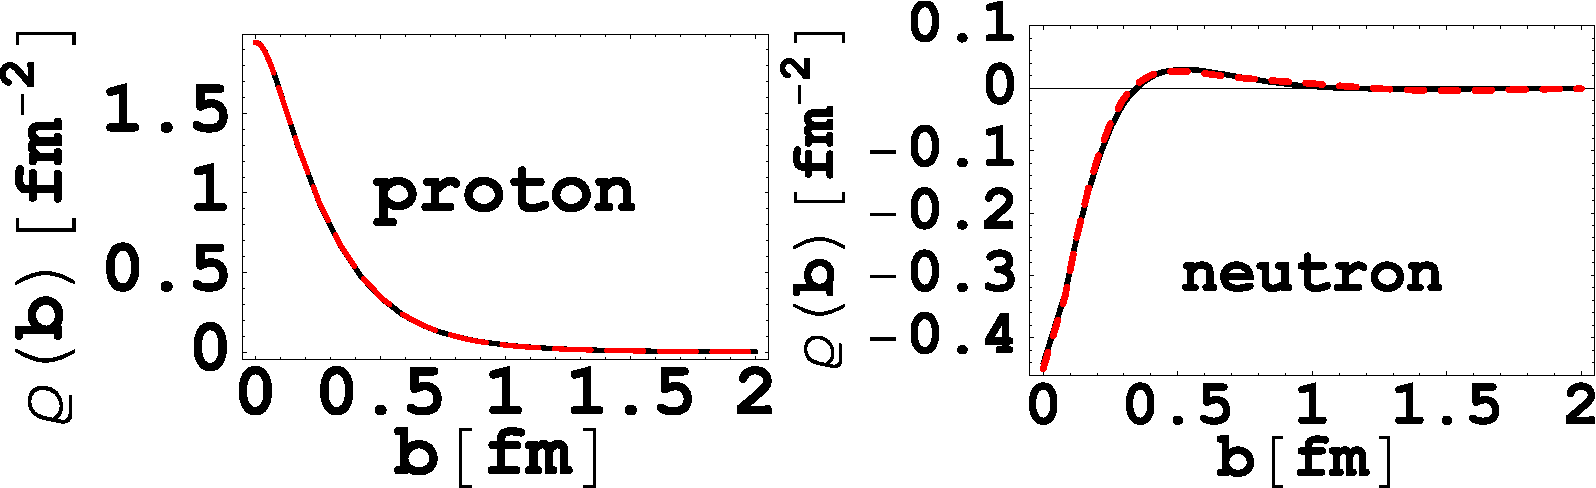
\includegraphics[width=0.9\linewidth]{charge_distribution_rotated}
	\caption{The proton charge density (left panel) and neutron charge density
		(right panel), taken from Ref.~\cite{miller2007}.}
	\label{fig:charge}
\end{figure}
These results further illustrate the internal structure of the nucleon.

In the 1960s, the quark model was proposed independently by Gell-Mann~\cite{gell-mann1964} and Zweig ~\cite{zweig1964a, zweig1964}
to understand the growing number of new particles discovered throughout the 1940s and 1950s.
In the quark model, the baryons are made up of three quarks and the mesons are made up
of a quark and an antiquark. They can be organized as shown in \cref{fig:Octet}.
The magnetic moment of the proton can then be expressed as the sum of the magnetic moment
from the individual quarks. The proton consists of $uud$ and the neutron consists of $udd$,
requiring the wavefunction to be symmetric in both flavor and spin, and the flavor-spin wavefunction of a proton with
spin up is given by
\begin{equation}
	\begin{split}
		\ket{p,\uparrow}= & \Bigl\{\frac{1}{2}\ket{\uparrow\downarrow\uparrow-\downarrow\uparrow\uparrow}\ket{udu-duu} + \frac{1}{2}\ket{\uparrow\uparrow\downarrow-\uparrow\downarrow\uparrow}\ket{uud-udu} \\
		                  & +\frac{1}{2}\ket{\uparrow\uparrow\downarrow-\downarrow\uparrow\uparrow}\ket{uud-duu}\Bigr\} \frac{\sqrt{2}}{3}.
	\end{split}
\end{equation}
And the magnetic moments are now given by
\begin{align}
	\mu_p & = \frac{4}{3}\mu_u-\frac{1}{3}\mu_d,  \\
	\mu_n & = -\frac{1}{3}\mu_u+\frac{4}{3}\mu_d.
\end{align}
If we also assumed that $u$ and $d$ quarks share the same mass, the quark model
then predicts the ratio $\mu_p/\mu_n=-2/3$ which is impressively close to the measured ratio of
\num{0.6849793(3)}~\cite{workman2022}.
\begin{figure}[h!]
	\centering
	\begin{subfigure}{0.45\linewidth}
		

\tikzset{every picture/.style={line width=0.75pt}} %set default line width to 0.75pt        

\begin{tikzpicture}[x=0.75pt,y=0.75pt,yscale=-1,xscale=1]
%uncomment if require: \path (0,585); %set diagram left start at 0, and has height of 585

%Shape: Regular Polygon [id:dp3461512214390913] 
\draw  [dash pattern={on 4.5pt off 4.5pt}] (360,280) -- (315,357.94) -- (225,357.94) -- (180,280) -- (225,202.06) -- (315,202.06) -- cycle ;
%Straight Lines [id:da7975119261953387] 
\draw    (140,280) -- (408,280) ;
\draw [shift={(410,280)}, rotate = 180] [color={rgb, 255:red, 0; green, 0; blue, 0 }  ][line width=0.75]    (10.93,-3.29) .. controls (6.95,-1.4) and (3.31,-0.3) .. (0,0) .. controls (3.31,0.3) and (6.95,1.4) .. (10.93,3.29)   ;
%Straight Lines [id:da49187250319695275] 
\draw    (270,420) -- (270,142) ;
\draw [shift={(270,140)}, rotate = 90] [color={rgb, 255:red, 0; green, 0; blue, 0 }  ][line width=0.75]    (10.93,-3.29) .. controls (6.95,-1.4) and (3.31,-0.3) .. (0,0) .. controls (3.31,0.3) and (6.95,1.4) .. (10.93,3.29)   ;
%Straight Lines [id:da04662903115423256] 
\draw    (225,275) -- (225,285) ;
%Straight Lines [id:da6078809997154113] 
\draw    (315,275) -- (315,285) ;
%Shape: Circle [id:dp2506066338504991] 
\draw  [fill={rgb, 255:red, 255; green, 255; blue, 255 }  ,fill opacity=1 ] (210.2,202.06) .. controls (210.2,193.88) and (216.83,187.26) .. (225,187.26) .. controls (233.17,187.26) and (239.8,193.88) .. (239.8,202.06) .. controls (239.8,210.23) and (233.17,216.86) .. (225,216.86) .. controls (216.83,216.86) and (210.2,210.23) .. (210.2,202.06) -- cycle ;
%Shape: Circle [id:dp49323091495562255] 
\draw  [fill={rgb, 255:red, 255; green, 255; blue, 255 }  ,fill opacity=1 ] (300.2,202.06) .. controls (300.2,193.88) and (306.83,187.26) .. (315,187.26) .. controls (323.17,187.26) and (329.8,193.88) .. (329.8,202.06) .. controls (329.8,210.23) and (323.17,216.86) .. (315,216.86) .. controls (306.83,216.86) and (300.2,210.23) .. (300.2,202.06) -- cycle ;
%Shape: Circle [id:dp2780130541001513] 
\draw  [fill={rgb, 255:red, 255; green, 255; blue, 255 }  ,fill opacity=1 ] (165.2,280) .. controls (165.2,271.83) and (171.83,265.2) .. (180,265.2) .. controls (188.17,265.2) and (194.8,271.83) .. (194.8,280) .. controls (194.8,288.17) and (188.17,294.8) .. (180,294.8) .. controls (171.83,294.8) and (165.2,288.17) .. (165.2,280) -- cycle ;
%Shape: Circle [id:dp22149042815123876] 
\draw  [fill={rgb, 255:red, 255; green, 255; blue, 255 }  ,fill opacity=1 ] (345.2,280) .. controls (345.2,271.83) and (351.83,265.2) .. (360,265.2) .. controls (368.17,265.2) and (374.8,271.83) .. (374.8,280) .. controls (374.8,288.17) and (368.17,294.8) .. (360,294.8) .. controls (351.83,294.8) and (345.2,288.17) .. (345.2,280) -- cycle ;
%Shape: Circle [id:dp2315285626329665] 
\draw  [fill={rgb, 255:red, 255; green, 255; blue, 255 }  ,fill opacity=1 ] (210.2,357.94) .. controls (210.2,349.77) and (216.83,343.14) .. (225,343.14) .. controls (233.17,343.14) and (239.8,349.77) .. (239.8,357.94) .. controls (239.8,366.12) and (233.17,372.74) .. (225,372.74) .. controls (216.83,372.74) and (210.2,366.12) .. (210.2,357.94) -- cycle ;
%Shape: Circle [id:dp3088315424845015] 
\draw  [fill={rgb, 255:red, 255; green, 255; blue, 255 }  ,fill opacity=1 ] (300.2,357.94) .. controls (300.2,349.77) and (306.83,343.14) .. (315,343.14) .. controls (323.17,343.14) and (329.8,349.77) .. (329.8,357.94) .. controls (329.8,366.12) and (323.17,372.74) .. (315,372.74) .. controls (306.83,372.74) and (300.2,366.12) .. (300.2,357.94) -- cycle ;
%Shape: Circle [id:dp27152267435822064] 
\draw  [fill={rgb, 255:red, 255; green, 255; blue, 255 }  ,fill opacity=1 ] (255.2,280) .. controls (255.2,271.83) and (261.83,265.2) .. (270,265.2) .. controls (278.17,265.2) and (284.8,271.83) .. (284.8,280) .. controls (284.8,288.17) and (278.17,294.8) .. (270,294.8) .. controls (261.83,294.8) and (255.2,288.17) .. (255.2,280) -- cycle ;
%Straight Lines [id:da5232366045305828] 
\draw    (265,202.1) -- (275,202.1) ;
%Straight Lines [id:da5088485977717139] 
\draw    (265,357.94) -- (275,357.94) ;

% Text Node
\draw (272,140) node [anchor=west] [inner sep=0.75pt]  [font=\large]  {$s$};
% Text Node
\draw (412,280) node [anchor=west] [inner sep=0.75pt]    {$I_{3}$};
% Text Node
\draw (270.5,190.65) node [anchor=north west][inner sep=0.75pt]  [font=\fontsize{0.71em}{0.85em}\selectfont]  {$0$};
% Text Node
\draw (271.08,360.57) node [anchor=north west][inner sep=0.75pt]  [font=\fontsize{0.71em}{0.85em}\selectfont]  {$-2$};
% Text Node
\draw (180,298.2) node [anchor=north] [inner sep=0.75pt]  [font=\fontsize{0.71em}{0.85em}\selectfont]  {$-1$};
% Text Node
\draw (360,298.2) node [anchor=north] [inner sep=0.75pt]  [font=\fontsize{0.71em}{0.85em}\selectfont]  {$+1$};
% Text Node
\draw (315.09,282.28) node [anchor=north] [inner sep=0.75pt]  [font=\fontsize{0.71em}{0.85em}\selectfont]  {$+\frac{1}{2}$};
% Text Node
\draw (224.65,282.6) node [anchor=north] [inner sep=0.75pt]  [font=\fontsize{0.71em}{0.85em}\selectfont]  {$-\frac{1}{2}$};
% Text Node
\draw (225,202.06) node    {$udd$};
% Text Node
\draw (315,202.06) node    {$uud$};
% Text Node
\draw (180,280) node    {$dds$};
% Text Node
\draw (270,280) node    {$uds$};
% Text Node
\draw (360,280) node    {$uus$};
% Text Node
\draw (225,357.94) node    {$dss$};
% Text Node
\draw (315,357.94) node    {$uss$};
% Text Node
\draw (225,183.86) node [anchor=south] [inner sep=0.75pt]    {$n$};
% Text Node
\draw (315,183.86) node [anchor=south] [inner sep=0.75pt]    {$p$};
% Text Node
\draw (225,374.14) node [anchor=north] [inner sep=0.75pt]    {$\Xi ^{-}$};
% Text Node
\draw (315,373.14) node [anchor=north] [inner sep=0.75pt]    {$\Xi ^{0}$};
% Text Node
\draw (172.38,276.82) node [anchor=south east] [inner sep=0.75pt]    {$\Sigma ^{-}$};
% Text Node
\draw (376.8,276.6) node [anchor=south west] [inner sep=0.75pt]    {$\Sigma +$};
% Text Node
\draw (263,269.6) node [anchor=south east] [inner sep=0.75pt]    {$\Sigma ^{0}$};
% Text Node
\draw (281,292.4) node [anchor=north west][inner sep=0.75pt]    {$\Lambda $};


\end{tikzpicture}


		\caption{The baryon spin 1/2 octet.}
	\end{subfigure}
	\hspace{3mm}%
	\begin{subfigure}{0.45\linewidth}
		

\tikzset{every picture/.style={line width=0.75pt}} %set default line width to 0.75pt        

\begin{tikzpicture}[x=0.75pt,y=0.75pt,yscale=-1,xscale=1]
%uncomment if require: \path (0,312); %set diagram left start at 0, and has height of 312

%Shape: Regular Polygon [id:dp00036259320032794307] 
\draw  [dash pattern={on 4.5pt off 4.5pt}] (230,162) -- (185,239.94) -- (95,239.94) -- (50,162) -- (95,84.06) -- (185,84.06) -- cycle ;
%Straight Lines [id:da7432714490785992] 
\draw [color={rgb, 255:red, 208; green, 2; blue, 27 }  ,draw opacity=1 ]   (10,162) -- (278,162) ;
\draw [shift={(280,162)}, rotate = 180] [color={rgb, 255:red, 208; green, 2; blue, 27 }  ,draw opacity=1 ][line width=0.75]    (10.93,-3.29) .. controls (6.95,-1.4) and (3.31,-0.3) .. (0,0) .. controls (3.31,0.3) and (6.95,1.4) .. (10.93,3.29)   ;
%Straight Lines [id:da5800138783290809] 
\draw [color={rgb, 255:red, 74; green, 144; blue, 226 }  ,draw opacity=1 ]   (140,302) -- (140,24) ;
\draw [shift={(140,22)}, rotate = 90] [color={rgb, 255:red, 74; green, 144; blue, 226 }  ,draw opacity=1 ][line width=0.75]    (10.93,-3.29) .. controls (6.95,-1.4) and (3.31,-0.3) .. (0,0) .. controls (3.31,0.3) and (6.95,1.4) .. (10.93,3.29)   ;
%Straight Lines [id:da0424063895802933] 
\draw [color={rgb, 255:red, 208; green, 2; blue, 27 }  ,draw opacity=1 ]   (95,157) -- (95,167) ;
%Straight Lines [id:da5315540321645463] 
\draw [color={rgb, 255:red, 208; green, 2; blue, 27 }  ,draw opacity=1 ]   (185,157) -- (185,167) ;
%Shape: Circle [id:dp9016274878129079] 
\draw  [fill={rgb, 255:red, 255; green, 255; blue, 255 }  ,fill opacity=1 ] (80.2,84.06) .. controls (80.2,75.88) and (86.83,69.26) .. (95,69.26) .. controls (103.17,69.26) and (109.8,75.88) .. (109.8,84.06) .. controls (109.8,92.23) and (103.17,98.86) .. (95,98.86) .. controls (86.83,98.86) and (80.2,92.23) .. (80.2,84.06) -- cycle ;
%Shape: Circle [id:dp26967635701794923] 
\draw  [fill={rgb, 255:red, 255; green, 255; blue, 255 }  ,fill opacity=1 ] (170.2,84.06) .. controls (170.2,75.88) and (176.83,69.26) .. (185,69.26) .. controls (193.17,69.26) and (199.8,75.88) .. (199.8,84.06) .. controls (199.8,92.23) and (193.17,98.86) .. (185,98.86) .. controls (176.83,98.86) and (170.2,92.23) .. (170.2,84.06) -- cycle ;
%Shape: Circle [id:dp829825410707284] 
\draw  [fill={rgb, 255:red, 255; green, 255; blue, 255 }  ,fill opacity=1 ] (35.2,162) .. controls (35.2,153.83) and (41.83,147.2) .. (50,147.2) .. controls (58.17,147.2) and (64.8,153.83) .. (64.8,162) .. controls (64.8,170.17) and (58.17,176.8) .. (50,176.8) .. controls (41.83,176.8) and (35.2,170.17) .. (35.2,162) -- cycle ;
%Shape: Circle [id:dp7821465181120492] 
\draw  [fill={rgb, 255:red, 255; green, 255; blue, 255 }  ,fill opacity=1 ] (215.2,162) .. controls (215.2,153.83) and (221.83,147.2) .. (230,147.2) .. controls (238.17,147.2) and (244.8,153.83) .. (244.8,162) .. controls (244.8,170.17) and (238.17,176.8) .. (230,176.8) .. controls (221.83,176.8) and (215.2,170.17) .. (215.2,162) -- cycle ;
%Shape: Circle [id:dp050740490078981626] 
\draw  [fill={rgb, 255:red, 255; green, 255; blue, 255 }  ,fill opacity=1 ] (80.2,239.94) .. controls (80.2,231.77) and (86.83,225.14) .. (95,225.14) .. controls (103.17,225.14) and (109.8,231.77) .. (109.8,239.94) .. controls (109.8,248.12) and (103.17,254.74) .. (95,254.74) .. controls (86.83,254.74) and (80.2,248.12) .. (80.2,239.94) -- cycle ;
%Shape: Circle [id:dp8501124972426272] 
\draw  [fill={rgb, 255:red, 255; green, 255; blue, 255 }  ,fill opacity=1 ] (170.2,239.94) .. controls (170.2,231.77) and (176.83,225.14) .. (185,225.14) .. controls (193.17,225.14) and (199.8,231.77) .. (199.8,239.94) .. controls (199.8,248.12) and (193.17,254.74) .. (185,254.74) .. controls (176.83,254.74) and (170.2,248.12) .. (170.2,239.94) -- cycle ;
%Shape: Circle [id:dp12490437005601918] 
\draw  [fill={rgb, 255:red, 255; green, 255; blue, 255 }  ,fill opacity=1 ] (119.65,162) .. controls (119.65,150.76) and (128.76,141.65) .. (140,141.65) .. controls (151.24,141.65) and (160.35,150.76) .. (160.35,162) .. controls (160.35,173.24) and (151.24,182.35) .. (140,182.35) .. controls (128.76,182.35) and (119.65,173.24) .. (119.65,162) -- cycle ;
%Straight Lines [id:da10691295631235598] 
\draw [color={rgb, 255:red, 74; green, 144; blue, 226 }  ,draw opacity=1 ]   (135,84.06) -- (145,84.06) ;
%Straight Lines [id:da40035051048673465] 
\draw [color={rgb, 255:red, 74; green, 144; blue, 226 }  ,draw opacity=1 ]   (135,239.9) -- (145,239.9) ;

% Text Node
\draw (142,22) node [anchor=west] [inner sep=0.75pt]  [font=\large,color={rgb, 255:red, 74; green, 144; blue, 226 }  ,opacity=1 ]  {$s$};
% Text Node
\draw (282,162) node [anchor=west] [inner sep=0.75pt]  [font=\large,color={rgb, 255:red, 208; green, 2; blue, 27 }  ,opacity=1 ]  {$I_{3}$};
% Text Node
\draw (140.5,72.65) node [anchor=north west][inner sep=0.75pt]  [font=\fontsize{0.71em}{0.85em}\selectfont,color={rgb, 255:red, 74; green, 144; blue, 226 }  ,opacity=1 ]  {$+1$};
% Text Node
\draw (141.08,242.57) node [anchor=north west][inner sep=0.75pt]  [font=\fontsize{0.71em}{0.85em}\selectfont,color={rgb, 255:red, 74; green, 144; blue, 226 }  ,opacity=1 ]  {$-1$};
% Text Node
\draw (50,180.2) node [anchor=north] [inner sep=0.75pt]  [font=\fontsize{0.71em}{0.85em}\selectfont,color={rgb, 255:red, 208; green, 2; blue, 27 }  ,opacity=1 ]  {$-1$};
% Text Node
\draw (230,180.2) node [anchor=north] [inner sep=0.75pt]  [font=\fontsize{0.71em}{0.85em}\selectfont,color={rgb, 255:red, 208; green, 2; blue, 27 }  ,opacity=1 ]  {$+1$};
% Text Node
\draw (185.09,164.28) node [anchor=north] [inner sep=0.75pt]  [font=\fontsize{0.71em}{0.85em}\selectfont,color={rgb, 255:red, 208; green, 2; blue, 27 }  ,opacity=1 ]  {$+\frac{1}{2}$};
% Text Node
\draw (94.65,164.6) node [anchor=north] [inner sep=0.75pt]  [font=\fontsize{0.71em}{0.85em}\selectfont,color={rgb, 255:red, 208; green, 2; blue, 27 }  ,opacity=1 ]  {$-\frac{1}{2}$};
% Text Node
\draw (95,84.06) node    {$d\overline{s}$};
% Text Node
\draw (185,84.06) node    {$u\overline{s}$};
% Text Node
\draw (50,162) node    {$\overline{u} d$};
% Text Node
\draw (230,162) node    {$u\overline{d}$};
% Text Node
\draw (95,239.94) node    {$\overline{u} s$};
% Text Node
\draw (185,239.94) node    {$\overline{d} s$};
% Text Node
\draw (95,65.86) node [anchor=south] [inner sep=0.75pt]    {$K^{0}$};
% Text Node
\draw (185,65.86) node [anchor=south] [inner sep=0.75pt]    {$K^{+}$};
% Text Node
\draw (95,256.14) node [anchor=north] [inner sep=0.75pt]    {$K^{-}$};
% Text Node
\draw (185,255.14) node [anchor=north] [inner sep=0.75pt]    {$\overline{K}^{0}$};
% Text Node
\draw (42.38,158.82) node [anchor=south east] [inner sep=0.75pt]    {$\pi ^{-}$};
% Text Node
\draw (246.8,158.6) node [anchor=south west] [inner sep=0.75pt]    {$\pi ^{+}$};
% Text Node
\draw (134.27,146.09) node [anchor=south east] [inner sep=0.75pt]    {$\pi ^{0}$};
% Text Node
\draw (147.6,178.55) node [anchor=north west][inner sep=0.75pt]    {$\eta $};
% Text Node
\draw (140,162) node  [font=\fontsize{0.8em}{0.96em}\selectfont] [align=left] {\begin{minipage}[lt]{24.07pt}\setlength\topsep{0pt}
\begin{center}
$\displaystyle u\overline{u}$\\$\displaystyle d\overline{d}$ $\displaystyle s\overline{s}$
\end{center}

\end{minipage}};


\end{tikzpicture}

		\caption{The meson spin 0 octet.}
	\end{subfigure}
	%\caption{Baryon and meson organized based on their charge(diagonal), strangeness(vertical) and isospin $I_3$(horizontal). }
	\caption{Baryon and meson octets in the quark model.
		The hadrons are organized based on their strangeness $S$ and isospin $I_3$.}
	\label{fig:Octet}
\end{figure}
These quarks would also carry a fractional charge ($+2/3$ for $u$, $s$ quarks and $-1/3$ for $d$ quarks) to
explain the charge of the baryons. Since fractional charged particles were never observed, and there was
no experimental evidence for free quarks, the quark model was not considered as physical, but merely a mathematical construct at the time.

\section{Deep Inelastic Scattering}
\label{sec:dis}
Direct evidence for the point-like constituents in the nucleon would come later from DIS
experiments~\cite{breidenbach1969}, where a high
energy lepton ($l$) is inelastically scattered off a hadron ($h$), as
illustrated in \cref{fig:DIS}.
\begin{equation}
	l + h \rightarrow l^\prime + X.
\end{equation}
\begin{figure}[htbp!]
	\centering
	%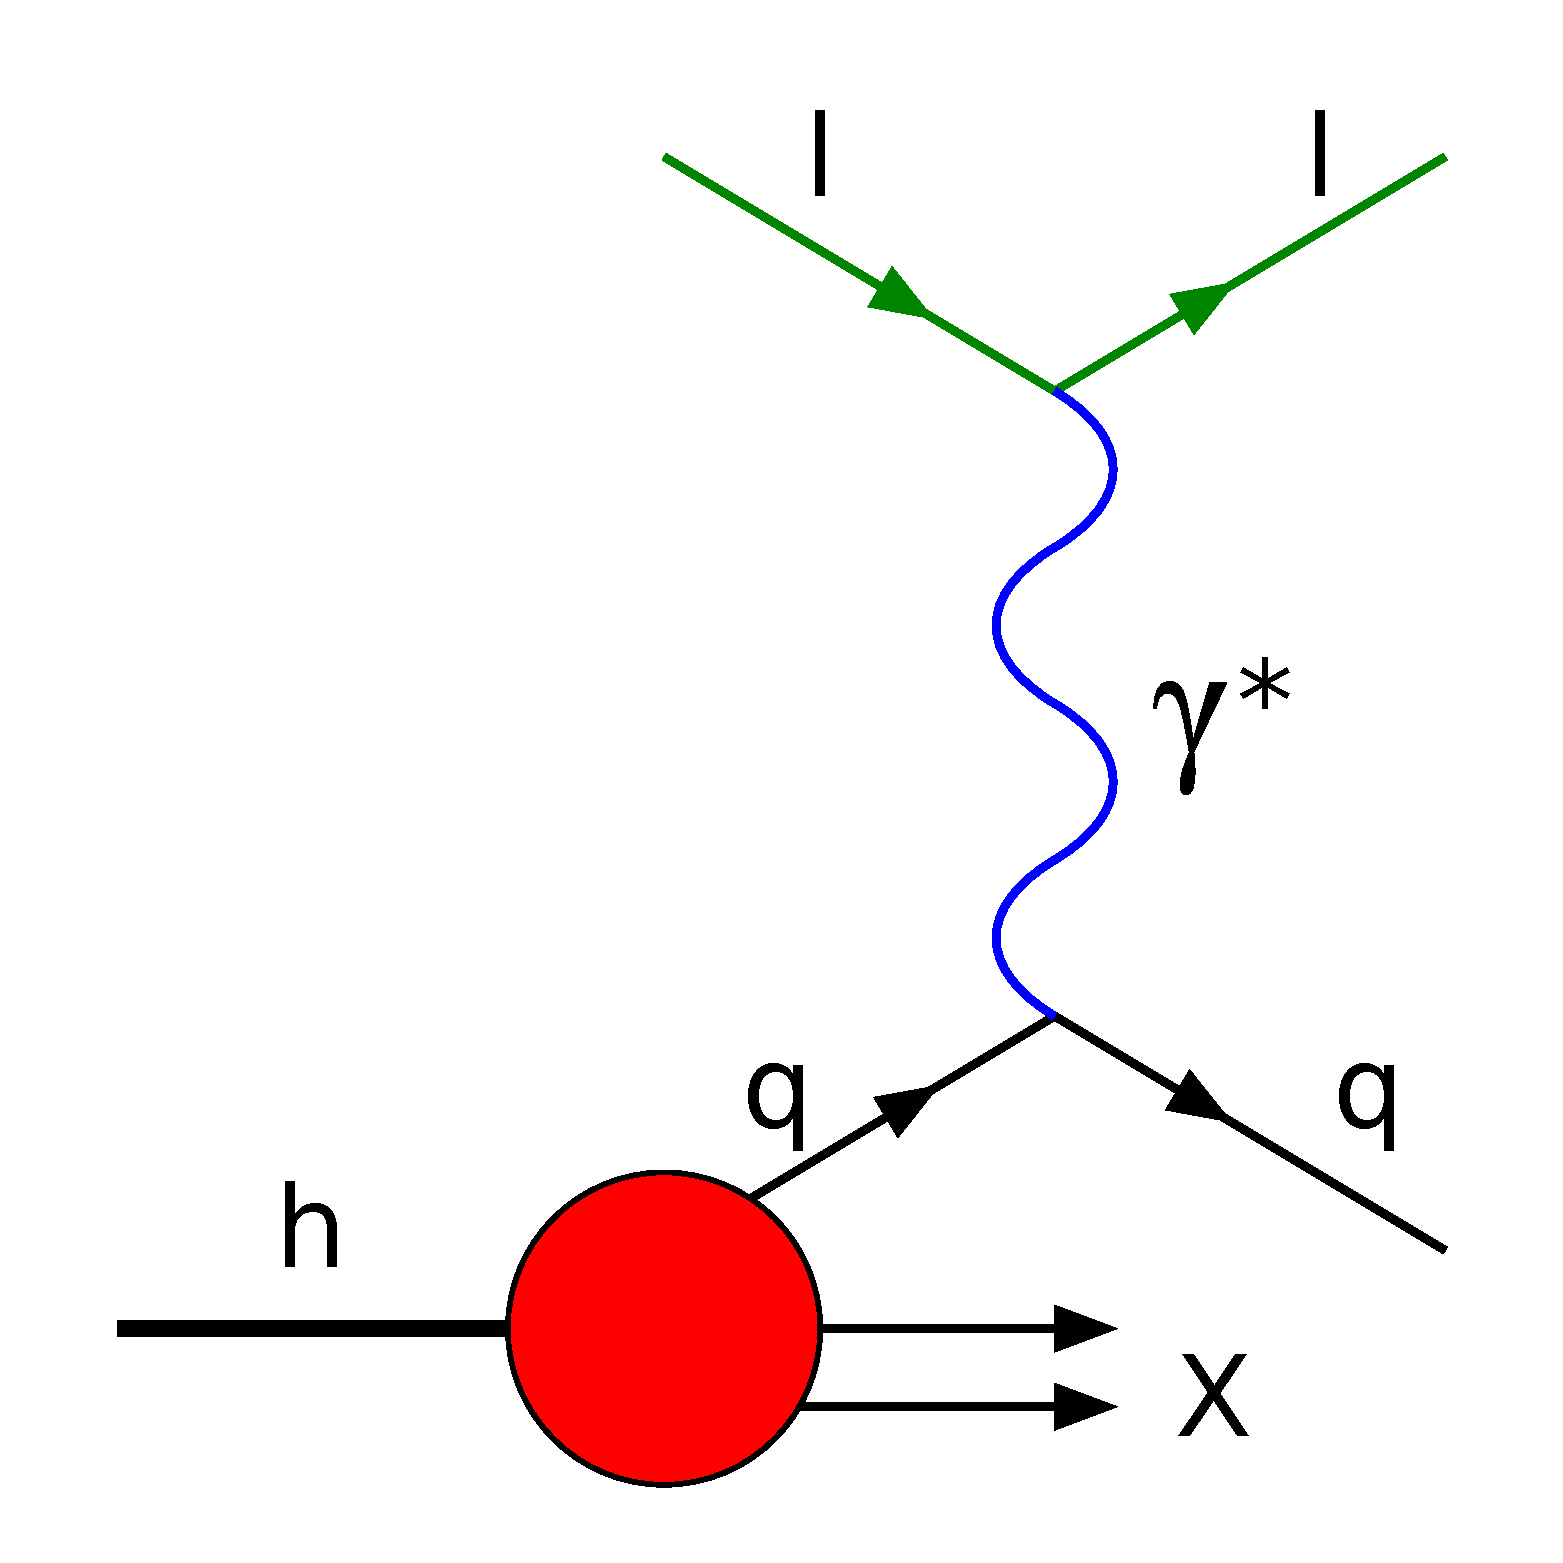
\includegraphics[width=0.3\linewidth]{DIS}
	\begin{tikzpicture}
	\tikzstyle{every node}=[font=\large]
	\begin{feynman}
		\vertex  (a1) {$l$};
		\vertex [right= 4cm of a1] (a2) {$l'$};

		\vertex [below= 4cm of a1,blob] (b2) {};
		\vertex [left= 1.2cm of b2] (b1) {$h$};
		\vertex[right= 2cm of b2] (b3){$X$};

		\vertex  at ($(a1) + (2cm , -1cm)$) [dot] (d);
		\vertex [below= 2 cm of d] (d1);

		\vertex at ($(d1) + (2cm, -1cm)$) (c1) {$q'$};
		
		\diagram*{
		(a1) --[fermion](d),
		(d)  --[fermion](a2),
		(b1) --[fermion](b2),
		(b2) --[fermion, edge label=$q$](d1),
		(d1) --[fermion](c1),
		(b2) --[double distance=4pt, thick](b3),
		(d) --[photon, edge label=$\gamma^*$](d1);
		};
	\end{feynman}
\end{tikzpicture}

	\caption{The Feynman diagram for DIS.}
	\label{fig:DIS}
\end{figure}
Similar to \cref{eq:ep_cs}, the DIS cross section can be expressed as
\begin{equation}
	\eval{\frac{d^2\sigma}{dE^\prime d\Omega}}_{DIS} = \frac{\alpha^2}{4E^2 \sin^4
		\frac{\theta}{2}} \left[ W_2\left(\nu,Q^2\right)\cos^2
		\frac{\theta}{2} + W_1\left(\nu,Q^2\right)\sin^2 \frac{\theta}{2}
		\right],
	\label{eq:DIS_cs1}
\end{equation}
where $\nu$ is the energy transferred by the scattering lepton.
In the elastic scattering, the cross section only depends on the momentum transfer squared $Q^2$,
as the energy transfer in $\nu$ is related to momentum transfer by $Q^2=2M\nu$.
In DIS, this relation no longer holds and the cross section would also depends on $\nu$.

It is also customary to define the structure functions $F_{1,2}$ from $W_{1,2}$ as:
\begin{equation}
	\begin{split}
		F_1\left(x,Q^2\right) & = MW_1\left(\nu,Q^2\right),    \\
		F_2\left(x,Q^2\right) & = \nu W_2\left(\nu,Q^2\right),
	\end{split}
\end{equation}
where $x=Q^2/2M\nu$ and $M$ is the mass of the nucleon. It was observed that at sufficiently high $Q^2$,
these structure functions $F_{1,2}$ are independent of $Q^2$, as illustrated in
\cref{fig:w2}. \Cref{fig:w2} shows the early measurements of the
structure function $F_2=\nu W_2$ as a function of $Q^2$ for a fixed
$x=1/\omega=0.25$ taken from Ref.~\cite{friedman1972}. This observation is
known as Bjorken scaling \cite{bjorken1969}.
\begin{figure}[htpb!]
	\centering
	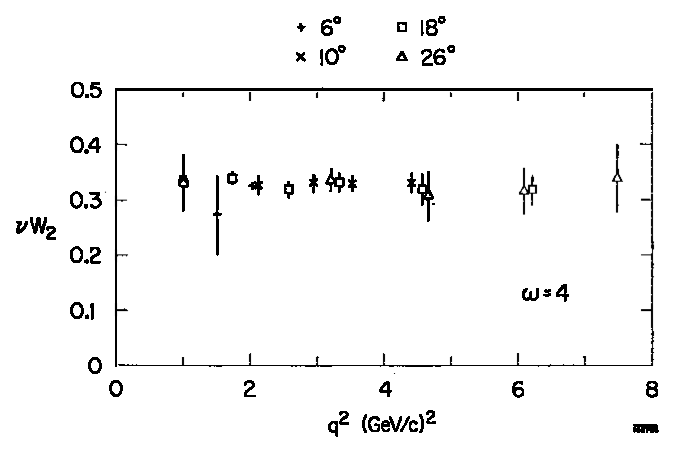
\includegraphics[width=0.5\linewidth]{nu_W2}
	\caption{Early measurement of the structure function $F_2=\nu W_2$ from
		fixed-target electron-proton deep inelastic scattering at SLAC for
		$x=1/\omega=0.25$, taken from Ref.~\cite{friedman1972}. The observation
		that $F_2(x,Q^2)$ is independent of $Q^2$ is known as Bjorken scaling. }
	\label{fig:w2}
\end{figure}
Taking the interpretation that the structure functions are related to the form factors in elastic scattering,
and therefore the Fourier transform of the charge distribution, the Bjorken scaling would suggest
the existence of point-like particles in the proton.

\section{Parton Model}
\label{sec:parton}
To explain the scaling behavior, Feynman proposed the parton model~\cite{feynman1969}.
In this model, hadrons are treated as extended objects which are made up of point-like
constituents (partons) held together by their mutual interaction. We now know
these partons are quarks and gluons described by QCD, but this was not known at
the time. Consider the DIS process, the hadron is Lorentz contracted in the
direction of the collision in the center-of-mass frame, and the internal
interaction are time dilated. As the center-of-mass energy increases, the
lifetime of the virtual partonic state is lengthened, and the time for the
electron to pass through the hadron is shortened. If the lifetime of the virtual
partonic states is longer than the duration of the electron-hadron interaction,
the partons are essentially frozen and the parton-parton interactions are
negligible. The hadrons can be considered as a collection of ``free'' partons,
and each parton may be thought of as carrying a certain fraction $x$ of the
hadron's momentum. The high energy lepton in DIS can be treated as scattering
off these partons elastically. The electron-parton elastic scattering can be
calculated using perturbative QCD, whereas the non-perturbative long-range
interaction within the hadron is encapsulated in the Parton Distribution
Function (PDF) $f_{a/h}\left(x\right)$, which can be interpreted as the probability
of finding a parton of species $a$ in hadron $h$ with fraction $x$ of the hadron's momentum.
And the cross section can be written as a convolution
of the non-perturbative PDF and the perturbative short range interaction. To leading
order (LO), the structure function $F_2\left(x,Q^2\right)$ is given by
\begin{equation}
	F_2\left(x,Q^2\right)=x\sum_i e^2_i f_{i/h}\left(x,Q^2\right),
	\label{eq:F2_parton}
\end{equation}
where $e_i$ is the charge carried by the quark and antiquark of flavor $i$. Since the
gluon does not carry any charge, it does not enter the cross section at leading
order. The ability to write the structure function and the cross section as a
convolution of the non-perturbative PDF and pertubative short range interaction
is known as the factorization theorem~\cite{collins1989}. These PDFs are also
expected to be universal and independent of the details of the scattering
process, as they describe the dynamics of the partons in a given hadron.

In the parton model, the structure functions $F_2$ and $F_1$ are clearly related. And
from \cref{eq:DIS_cs1}, the structure function $F_1$ is
related to the magnetic form factor $G_M$ in \cref{eq:ep_cs}. If the partons
are spin 0 particles, one would expect $F_1$ to be zero. In leading order of QCD,
only the quarks and antiquarks contribute to the cross section. Since quarks and
antiquarks are spin 1/2 particles, $F_1$ and $F_2$ are expected to satisfy the Callan-Gross
relation~\cite{callan1968,callan1969}
\begin{equation}
	F_2\left(x,Q^2\right) = 2x F_1\left(x,Q^2\right).
	\label{eq:CS_relation}
\end{equation}
The measured deviation from the Callan-Gross relation, defined as
\begin{equation}
	K_0 = \frac{F_2}{2xF_1}-1,
\end{equation}
is shown in \cref{fig:callan_gross}, taken from Ref.~\cite{kendall1991}.
For large $Q^2$, $K_0$ is consistent with zero, establishing the spin of the
charged partons is 1/2.
The deviation at low $Q^2$ is expected from the QCD corrections and contributions from
the gluons.
\begin{figure}[htbp!]
	\centering
	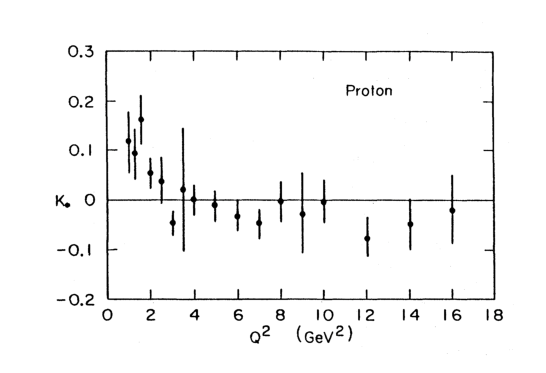
\includegraphics[width=0.5\linewidth]{Callan_Gross_relation}
	\caption{The deviation from the Callan-Gross relation, defined as
		$K_0=F_2/2xF_1 -1$, taken from Ref.~\cite{kendall1991}. This result
		demonstrates the spin 1/2 nature of the partons.}
	\label{fig:callan_gross}
\end{figure}

\section{Sum Rules}
\label{sec:sum_rules}
Since hadrons are characterized by their quantum numbers, hadrons consist of partons,
these quantum numbers serve as constraints on these PDFs.
For example, from the number of valence quarks in the proton,
one can impose the following constraints
\begin{equation}
	\begin{split}
		\int_{0}^{1} \dd{x} \left[f_{u/p} \left(x\right)-f_{\bar{u}/p} \left(x\right)\right] & =2,                                          \\
		\int_{0}^{1} \dd{x} \left[f_{d/p} \left(x\right)-f_{\bar{d}/p} \left(x\right)\right] & =1,                                          \\
		\int_{0}^{1} \dd{x} \left[f_{i/p} \left(x\right)-f_{\bar{i}/p} \left(x\right)\right] & =0 \qquad \text{for other quark flavors } i.
	\end{split}
\end{equation}
And the momentum of the hadron should be shared among the partons, hence
\begin{equation}
	\sum_{i=u,d,s,\cdots} \int_{0}^{1}\dd{x}\left[x f_{i/p}\left(x\right) +x f_{\bar{i}/p}\left(x\right) \right] + \int_{0}^{1}\dd{x} x f_{g/p}\left(x\right)=1
\end{equation}
An important sum rule is the Gottfried sum rule~\cite{gottfried1967}. It can be obtained
by using the charge symmetry,
which is the invariance under $u\leftrightarrow d$ and $\bar{u}\leftrightarrow \bar{d}$ interchange,
to relate the neutron distributions to those of
the proton, namely
\begin{equation}
	\begin{split}
		\bar{u}(x) \equiv f_{\bar{u}/p}(x) = f_{\bar{d}/n}(x); & \quad u(x) \equiv f_{u/p}(x) = f_{d/n}(x); \\
		\bar{d}(x) \equiv f_{\bar{d}/p}(x) = f_{\bar{u}/n}(x); & \quad d(x) \equiv f_{d/p}(x) = f_{u/n}(x).
	\end{split}
\end{equation}
The other quarks flavors and gluon distribution would be the same in both proton and neutron.
Using these relations and \cref{eq:F2_parton}, one obtains
\begin{equation}
	\begin{split}
		S_G & = \int_0^1 \frac{\dd{x}}{x}\left(F_2^{p}(x) - F_{2}^{n}(x)\right)                                     \\
		    & = \frac{1}{3} \int_0^1 \dd{x} \left[u\left(x\right) - d\left(x\right)
		+ \bar{u}\left(x\right) - \bar{d}\left(x\right)\right]                                                      \\
		    & = \frac{1}{3} \int_0^1 \dd{x} \left[u\left(x\right) - \bar{u}\left(x\right)\right]
		- \frac{1}{3} \int_0^1 \dd{x} \left[d\left(x\right) - \bar{d}\left(x\right)\right]
		+ \frac{2}{3} \int_0^1 \dd{x} \left[\bar{u}\left(x\right)-\bar{d}\left(x\right)\right]                      \\
		    & = \frac{1}{3} + \frac{2}{3} \int_0^1 \dd{x} \left[\bar{u}\left(x\right)-\bar{d}\left(x\right)\right].
	\end{split}
\end{equation}
If one assumes that $\bar{u}\left(x\right)= \bar{d}\left(x\right)$,
then $S_G$ would be $1/3$. This assumption can be tested using DIS.
One of the early measurements is from the New Muon Collaboration (NMC)~\cite{amaudruz1991}.
The $F_2^p-F_2^n$ measured by NMC is shown in \cref{fig:NMC_Gottfried}.
\begin{figure}[htbp!]
	\centering
	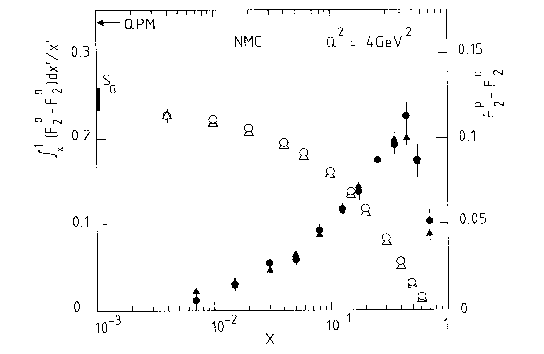
\includegraphics[width=0.7\linewidth]{Gottfried}
	\caption{The difference $F_2^p -F_2^n$ (solid and scale to the right) and
		$\int_{x_{min}}^1 (F_2^p-F_2^n)\dd{x}/x$ (open and scale to the left)
		determined by NMC, taken from Ref.~\cite{amaudruz1991}. The extrapolation
		to $x_{min}=0$ is indicated by the bar on the left vertical axis.}
	\label{fig:NMC_Gottfried}
\end{figure}
The extracted Gottfried sum is $0.240 \pm 0.016$, which is significantly below
$1/3$, suggesting an asymmetry in the light sea-quarks, $\bar{d}(x)\neq \bar{u}(x)$.

\section{Quantum Chromodynamics}
\label{sec:QCD}
\pdfmargincomment{General QCD}
Quantum Chromodynamics (QCD) is a theory of the strong interaction. It was
introduced by Fritzsch and Gell-Mann~\cite{fritzsch1972} and Fritzsch, Gell-Mann,
and Leutwyler~\cite{fritzsch1973}. QCD is a non-abelian gauge theory with an
$SU(3)$ gauge symmetry applied to the color degree of freedom. The $SU(3)$ group
chosen to account for (a) meson states made up of $q\bar{q}$ but not $qq$ bound states.
(b) There must be color singlet states. (c) The number of colors for each flavor
must be in agreement with the measured hadronic cross-section in $e^+ e^-$ collision.

An important feature of QCD is the asymptotic freedom. Being a renormalizable
theory, a regularization procedure and a set of renormalization prescription
need to be specified. In the renormalization process, the renormalized coupling $\alpha(\mu)$
is introduced and this coupling would be a function of the renormalization scale $\mu$.
It is noted that the coupling constant vanishes as $Q/\mu$ tends to infinity~\cite{gross1973,politzer1973},
allowing perturbative expansion of QCD at large $Q$.


\subsection{QCD Improved Parton Model and Scaling Violation}
\label{subsec:scaling_violation}
In QCD, the parton distribution functions can be defined as matrix elements of
operators acting on the hadron state. These operators act to count the number of
quarks and gluons carrying a fraction $\xi$ of the hadron's momentum. For quarks,
the distribution is given by~\cite{collins1989}
\begin{equation}
	f_{q/h}\left(\xi\right) = \frac{1}{4\pi}\int \dd{x} e^{-i\xi P^{+} x^{-}} \mel{P}{\bar{\psi}\left(0,x^-,0_\perp\right)\gamma^+ \mathcal{G} \psi\left(0,0,0_\perp\right)}{P},
\end{equation}
where $\mathcal{G}$ is the gauge link operator
\begin{equation}
	\mathcal{G}=\mathcal{P} \exp \left\{ ig\int_0^{x^-}\dd{y^-} A_c^+ \left(0,y^-,0_\perp\right)t_c\right\},
\end{equation}
where $\mathcal{P}$ denoted the path ordering of the gluon field operators $A_c^+$
along the path. Similarly, the gluon distribution function is given by
\begin{equation}
	f_{g/h}\left(\xi\right) = \frac{1}{2\pi\xi P^+}\int \dd{x} e^{-i\xi P^{+} x^{-}} \mel{P}{\tensor{F_a\left(0,x^-,0_\perp\right)}{^+^\nu} \tensor{\mathcal{G}}{_a_b} \tensor{F_b\left(0,0,0_\perp\right)}{_\nu^+}}{P},
\end{equation}
where $F^a_{\mu\nu}$ is the field tensor operator, and the octet representation of the $SU(3)$
generating matrices $t_c$ is used in $\mathcal{G}$.

The QCD generalization of \cref{eq:F2_parton} is
\begin{equation}
	\frac{1}{x}F_2\left(x,Q^2\right) = \sum_a \int_x^1 \frac{\dd{\xi}}{x}f_{a/h}\left(\xi,\mu\right)\frac{\xi}{x}H_{2a}\left( \frac{x}{\xi}, \frac{Q}{\mu}, \alpha_s\left(\mu\right)\right)
	+ \text{Remainder}.
\end{equation}
The hard scattering coefficient $H_{2a}$ is expanded as power series in $\alpha_s$. It
can be shown that the remainder is suppressed by powers of $Q$. Here the parton
distribution also depends on the renormalization scale $\mu$. This scale
dependency is introduced by the renormalization procedure. By requiring the cross
section and the structure functions to be independent of the scale $\mu$,
one can show that the renormalization group equation for the distribution
functions is
\begin{equation}
	\mu\frac{d}{d\mu}f_{a/h}\left(\xi,\mu\right)=\sum_b \int_\xi^1 \frac{\dd{\zeta}}{\zeta} P_{a/b}\left(\zeta,\alpha_s\left(\mu\right)\right) f_{b/h}\left(\frac{\xi}{\zeta},\mu\right),
\end{equation}
where $P_{a/b}$ is the Altarelli-Parisi kernel~\cite{altarelli1977}.

At order $\alpha_s$, the $F_2$ structure function is given by~\cite{collins1989}
\begin{equation}
	\frac{1}{x} F_2\left(x,Q^2\right) = \sum_j e^2_j f_{j/h}\left(x,\mu\right) + \sum_{j,b} e^2_j \int^1_x \frac{\dd{\xi}}{\xi} f_{b/h}\left(\xi,\mu\right) \frac{\alpha_s}{\pi} C_{jb}\left(\frac{x}{\xi}, \frac{Q}{\mu}\right) + \mathcal{O}(\alpha_s^2).
\end{equation}
The sum over $j$ runs over the quark and antiquark flavors. While the gluons
did not contribute at leading order, they contribute at order $\alpha_s$ through
virtual quark-antiquark pairs. The hard scattering coefficients $C_{jb}$ are
given by
\begin{align}
	C_{jk}(z,1) & = \delta_{jk} \frac{4}{3} \left[ -\frac{1}{2}\frac{1+z^2}{1-z} \ln\left(\frac{z}{1-z}\right) + \frac{3}{4} \frac{1}{1-z} -\frac{3}{2} -z\right]_+ \\
	C_{jg}(z,1) & = -\frac{1}{2} \left\{ \frac{1}{2}\left[z^2+(1-z)^2\right] \left[\ln\left(\frac{z}{1-z}\right)+1\right] -3z(1-z)\right\},
\end{align}
where the plus subscript denotes the subtraction that regulates the $z\rightarrow1$
singularity,
\begin{equation}
	\begin{split}
		\int^1_x \dd{z} \left[C(z)\right]_+ h(z) & = \int_0^1 \dd{z} \left[C(z)\right]_+ h(z)\Theta(z>x)        \\
		                                         & = \int_0^1 \dd{z} C(z) \left\{h(z)\Theta(z>x) -h(1)\right\}.
	\end{split}
\end{equation}

It is customary to choose $\mu =Q$ to avoid large logarithms of $\mu /Q$ in the
power expansions of $H$. As such the $\mu$ dependency in the parton distribution
functions can be interpreted as a virtual photon with higher $Q$ would probe the
nucleon with better resolution.

\Cref{fig:DIS_scaling} shows the extracted $F_2$ from DIS measurements compared
with the NLO calculation. The $Q^2$ dependency is known as scaling violation and
originates from higher order corrections and $Q$ dependency of the PDF.
\begin{figure}[h!]
	\centering
	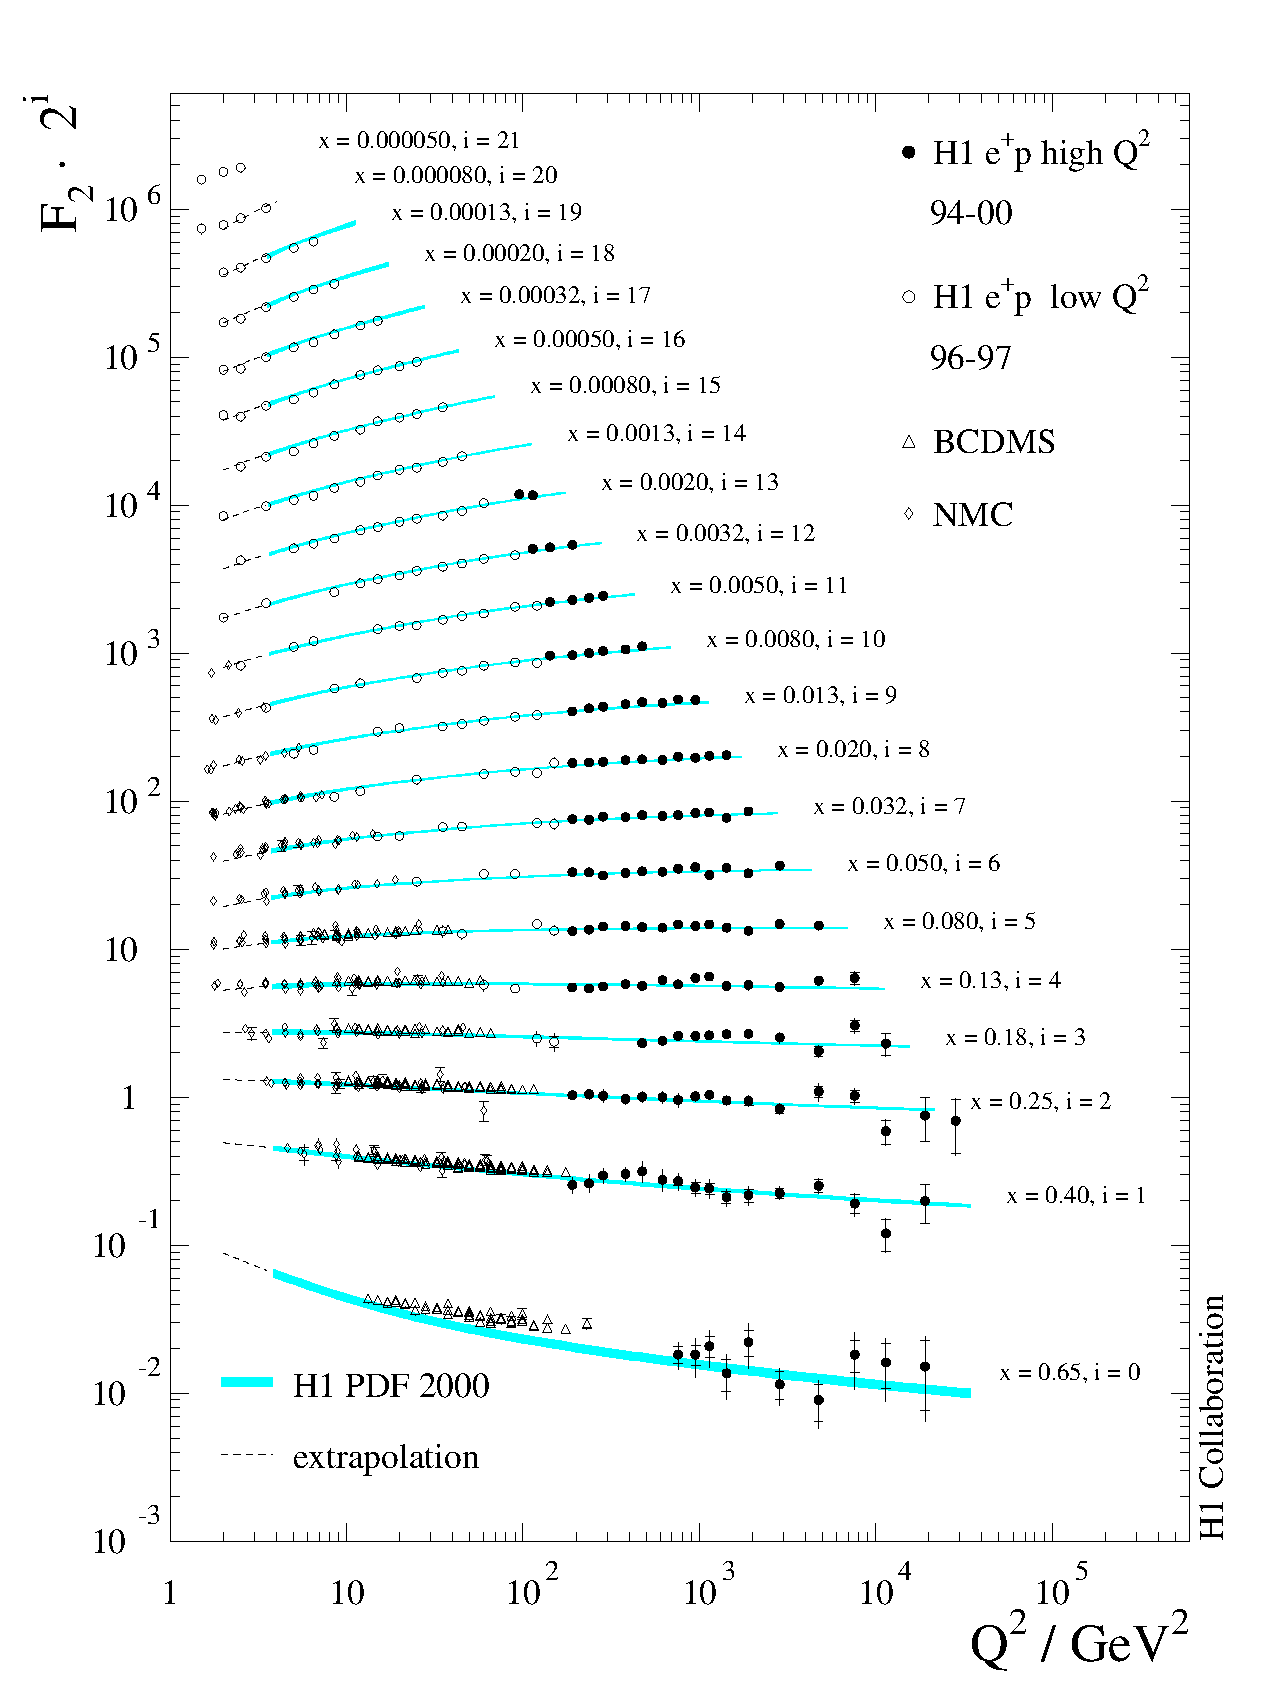
\includegraphics[width=0.6\linewidth]{DIS_scaling}
	\caption{
		Compilation of data on DIS, and compared with NLO calculations,
		taken from Ref.~\cite{adloff2003}.
		The $Q^2$ dependency is known as scaling violation,
		and originates from higher order corrections and $Q$ dependency of the PDF.
	}
	\label{fig:DIS_scaling}
\end{figure}
The Gottfried Sum Rule introduced in \cref{sec:sum_rules} would also be modified due to
QCD effects. At order $\alpha_s^2$, in the limit of a symmetric sea, the Gottfried Sum Rule
is given by~\cite{kataev2003}
\begin{equation}
	I_{GSR} = \begin{cases}
		\frac{1}{3}\left[ 1 + 0.0355\left(\frac{\alpha_s}{\pi}\right)-0.811\left(\frac{\alpha_s}{\pi}\right)^2 \right] & n_f=3, \\
		\frac{1}{3}\left[ 1 + 0.0384\left(\frac{\alpha_s}{\pi}\right)-0.822\left(\frac{\alpha_s}{\pi}\right)^2 \right] & n_f=4,
	\end{cases}
\end{equation}
where $n_f$ is the active flavor.
Taking $\alpha_s(Q^2=\SI{4}{\GeV^2})\approx 0.35$, the numerical value is $\approx 0.3313$. Therefore,
the light sea-quark asymmetry is still needed to explain the NMC result.

\Cref{fig:CT18_scale} shows the PDF extracted by CTEQ-TEA collaboration in their
CT18 global analysis~\cite{hou2021}. The sea-quarks from the gluon splitting
can be seen at low $x$ and is more important at large $Q$. This demonstrate the
QCD evolution of the PDF.

\begin{figure}
	\centering
	\begin{subfigure}{0.48\linewidth}
		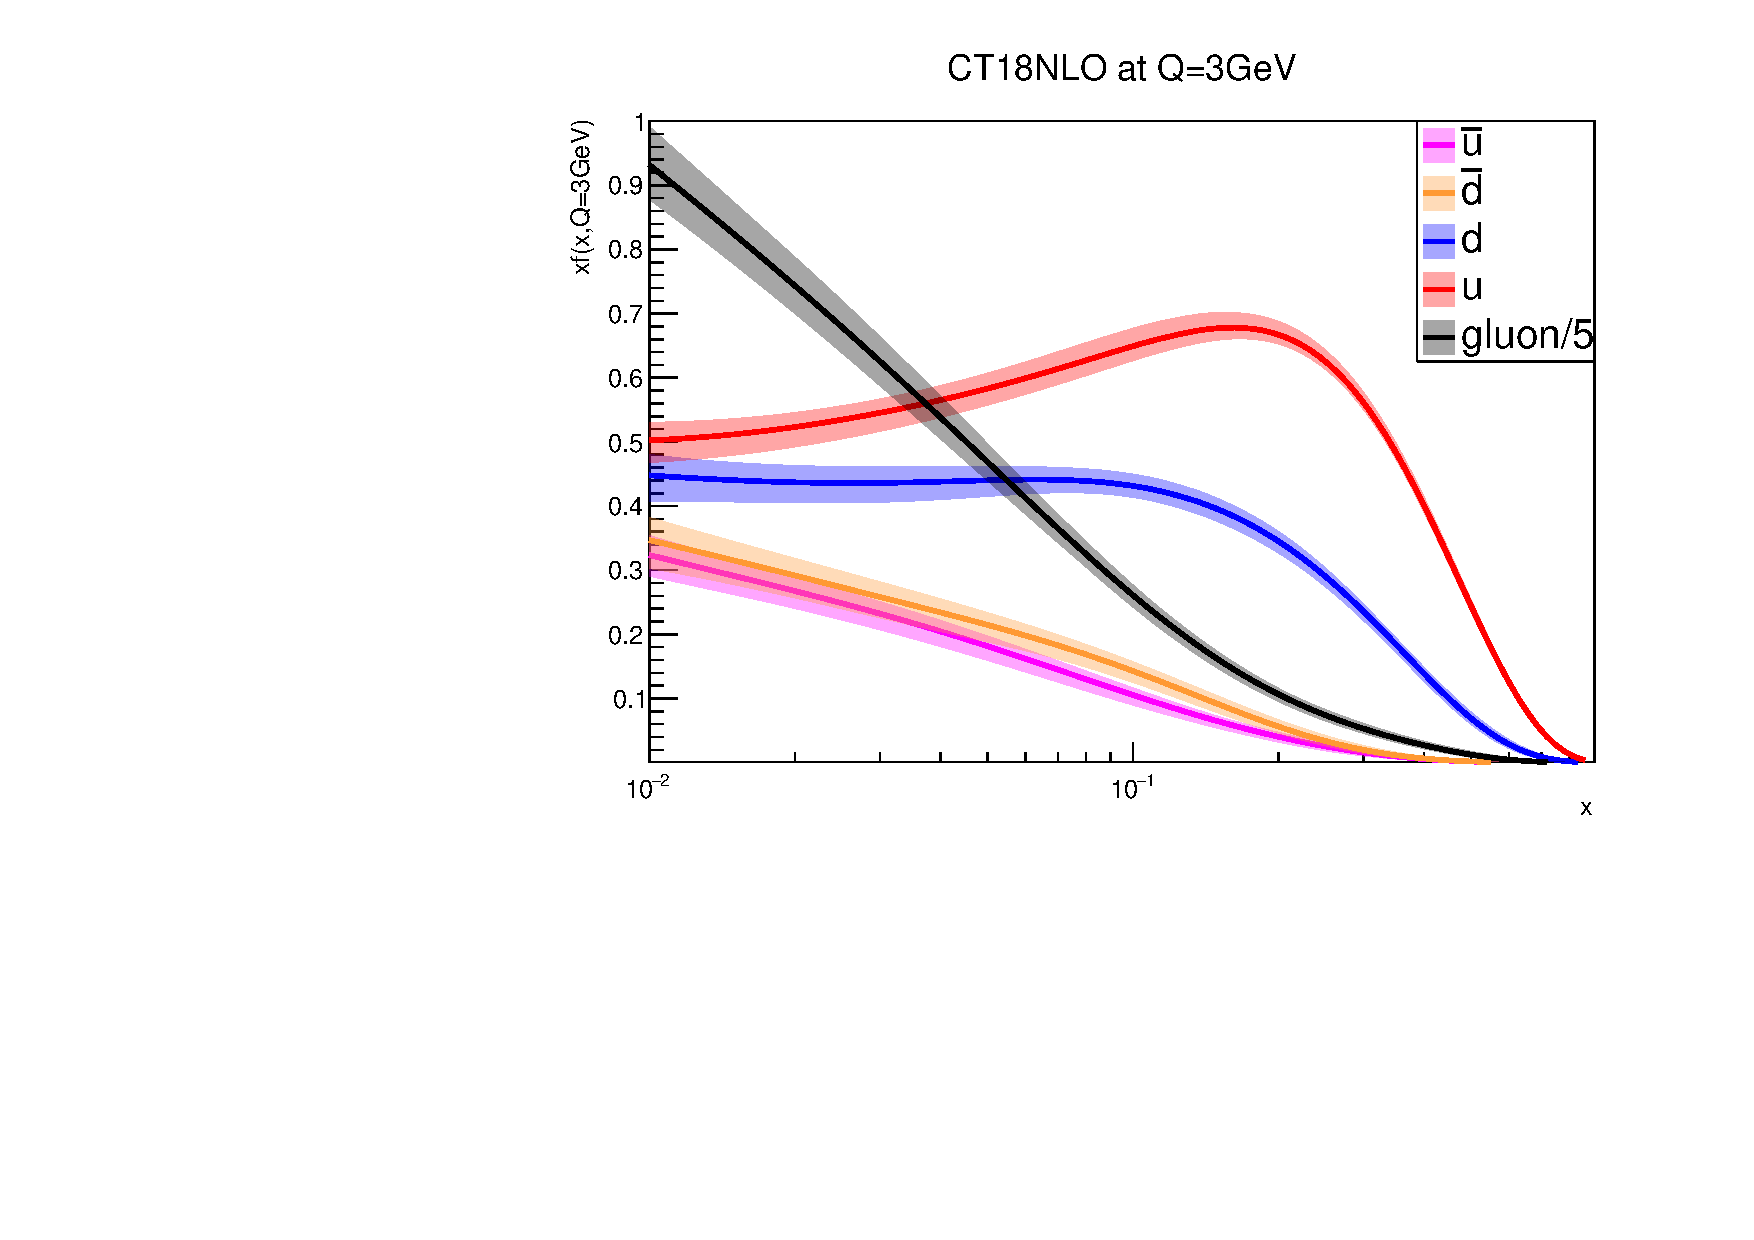
\includegraphics[width=\linewidth]{CT18NLO}
	\end{subfigure}
	\begin{subfigure}{0.48\linewidth}
		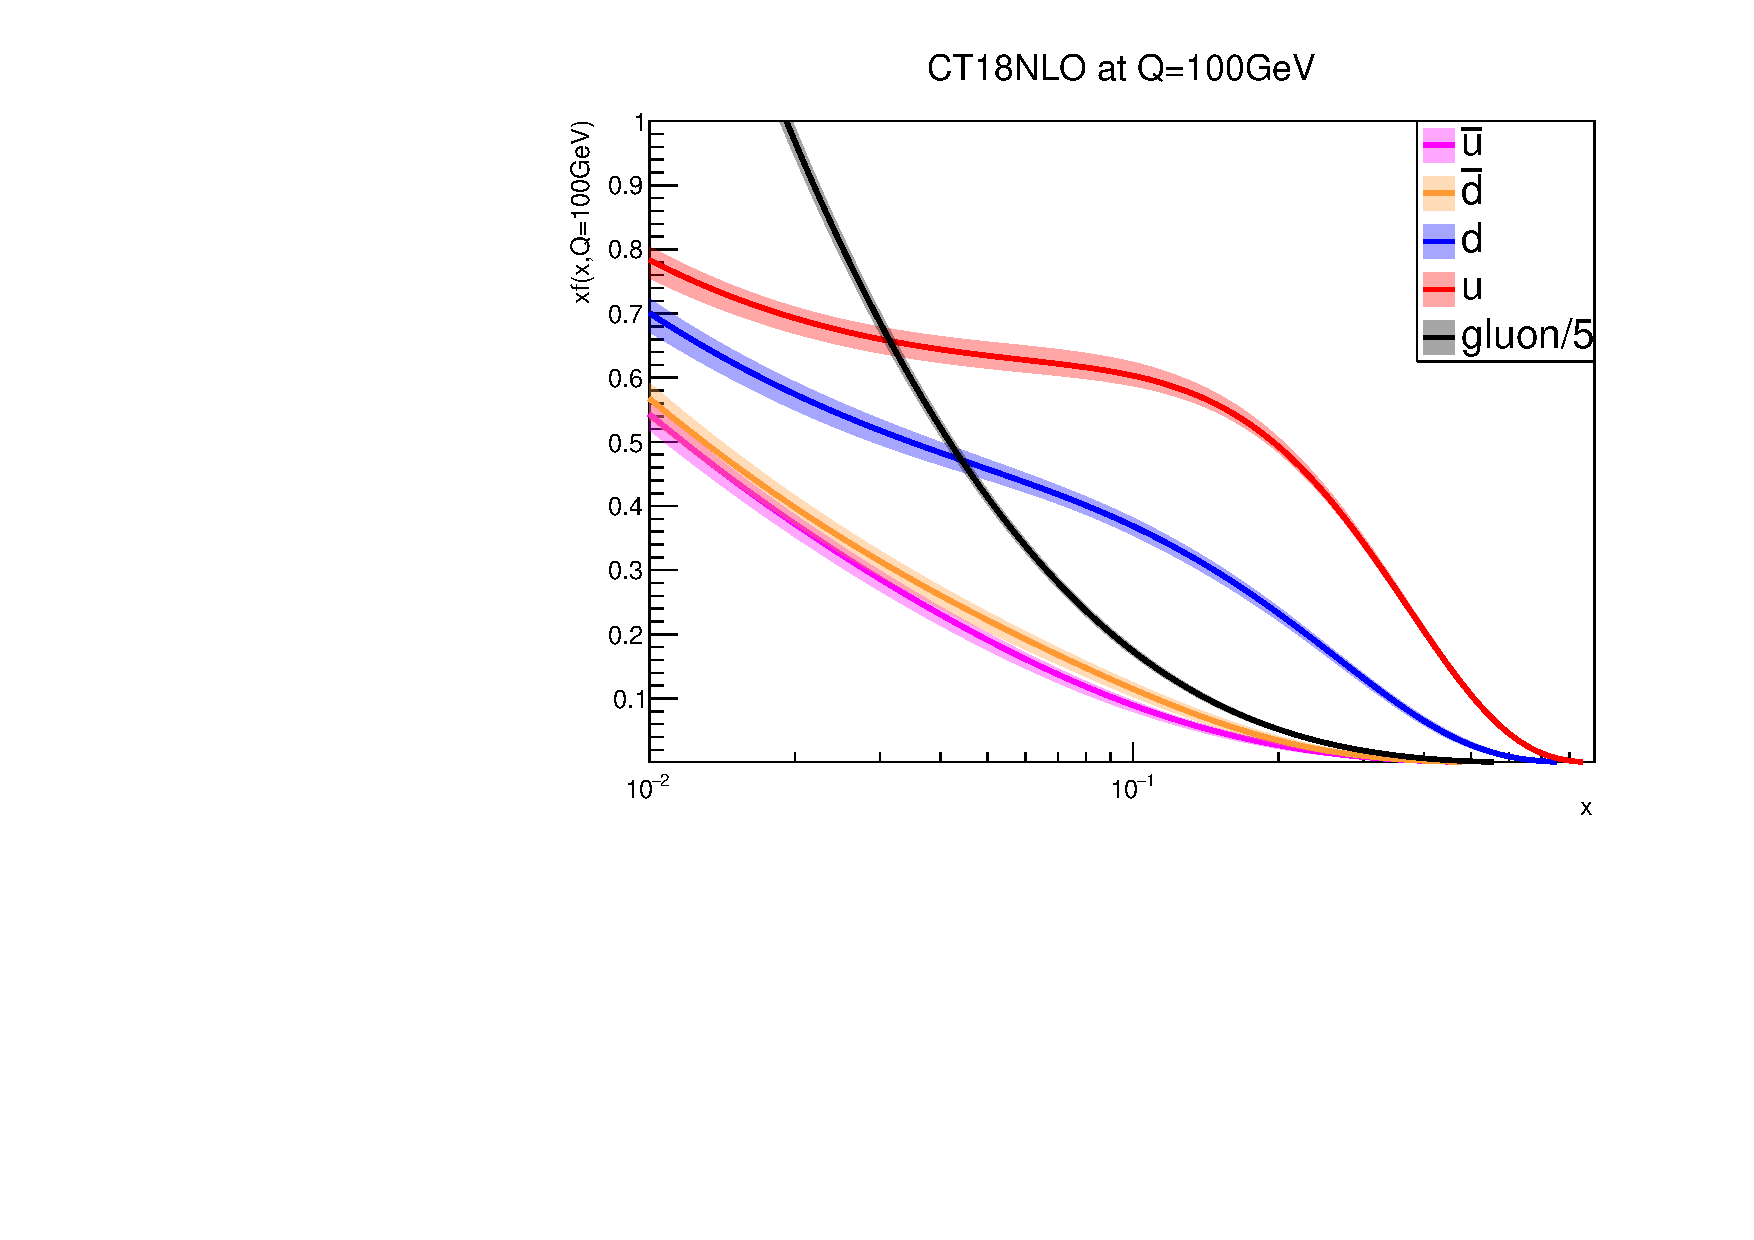
\includegraphics[width=\linewidth]{CT18NLO_100}
	\end{subfigure}
	\caption{The parton distribution functions from CT18~\cite{hou2021} global analysis at two different scales.
		The gluon distribution is scaled down by a factor of 5.}
	\label{fig:CT18_scale}
\end{figure}


\chapter{Drell-Yan Process}
\label{ch:DY}
In addition to DIS, another process for probing the hadron structure is the Drell-Yan process~\cite{drell1970}.
As illustrated in \cref{fig:DY}, this process involves two partons from the
two colliding hadrons to annihilate and form a lepton pair:
\begin{equation}
	h_A + h_B \rightarrow l + \bar{l} + X.
\end{equation}
The Drell-Yan process is related to the DIS process via crossing symmetry.
\begin{figure}[htbp!]
	\centering
	%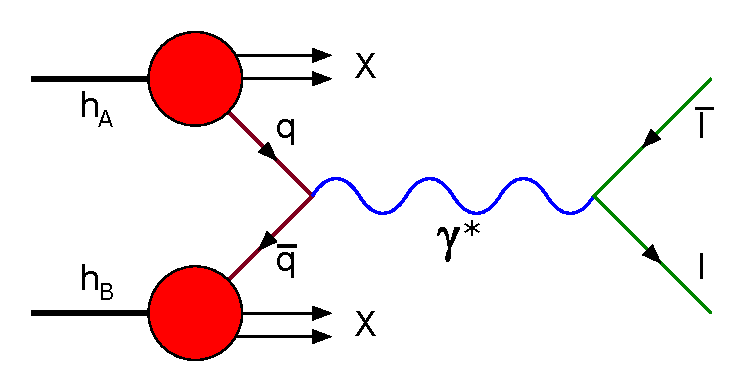
\includegraphics[width=0.5\linewidth]{Drell-Yan}
	\begin{tikzpicture}
	\tikzstyle{every node}=[font=\large]
	\begin{feynman}
		\vertex  (a1) {$h_A$};
		\vertex [right= of a1, blob] (a2) {};
		\vertex [right= 2cm of a2] (a3) {$X$};
		\vertex [below= 3cm of a1] (b1) {$h_B$};
		\vertex [below= 3cm of a2,blob] (b2) {};
		\vertex[below= 3cm of a3] (b3) {$X$};
		\vertex  at ($(b2) + (1.5cm , +1.5cm)$) [dot] (d);
		\vertex [right= 2.5 cm of d] (d1);
		\vertex at ($(d1) + (1.5cm , +1.2cm)$) (c1) {$l$};
		\vertex at ($(d1) + (1.5cm , -1.2cm)$) (c2) {$\bar{l}$};
		\diagram*{
		(a1) --[fermion](a2),
		(a2) --[double distance=4pt, thick](a3),
		(b1) --[fermion](b2),
		(b2) --[double distance=4pt, thick](b3),
		(d) --[fermion, edge label=$\bar{q}$] (b2),
		(a2) --[fermion, edge label=$q$](d),
		(d) --[photon, edge label=$\gamma^*$](d1),
		(c2) --[fermion] (d1);
		(d1) --[fermion] (c1);
		};
	\end{feynman}
\end{tikzpicture}

	\caption{The leading order Feynman diagram for the Drell-Yan process.}
	\label{fig:DY}
\end{figure}
Similar to DIS, the Drell-Yan cross section can be factorized into the non-perturbative
PDF and the perturbative parton-parton scattering. And the proof of factorization
theorem for Drell-Yan can be found in Ref.~\cite{collins1989}. At leading-order,
the cross section can be written as
\begin{equation}
	\frac{d^2\sigma_{DY}}{dx_{1}dx_{2}} = \frac{4\pi\alpha^2}{9M^2}\sum_q e^2_q
	\left[f_{q/A}\left(x_1\right)f_{\bar{q}/B}\left(x_2\right) +
	f_{\bar{q}/A}\left(x_1\right)f_{q/B}\left(x_2\right)
	\right],
	\label{eq:DY_cs}
\end{equation}
where $M$ is the mass of the lepton pair, $x_1$ and $x_2$ are the momentum fractions
carried by the partons from the two colliding hadrons. To simplify the notation,
the $Q^2$ scale dependence of the PDF is omitted here. In fixed target environments,
the scale $Q^2$ is typically chosen to the dilepton mass squared $M^2$.
The mass of the lepton pair and momentum fractions are related through
\begin{equation}
	M^2= sx_1x_2,
	\label{eq:mass}
\end{equation}
where $s$ is the hadron-hadron center-of-mass energy squared.
Since the underlying mechanism for the Drell-Yan process at leading order involves the annihilation
of a quark and an antiquark, this process is particularly useful in probing the antiquark
content of the hadron.
In the parton model, the angular distribution of the Drell-Yan dilepton would have the following
distribution from the decay of the transversely polarized virtual photon,
\begin{equation}
	\dv{\sigma_{DY}}{\Omega} = \sigma_0(1+\lambda \cos^2\theta),
\end{equation}
where $\theta$ is the polar angle of the lepton in the virtual photon rest frame and $\lambda=1$.

The Drell-Yan process and the parton model has been successful in explaining the shape of
the dimuon production cross section and the angular distribution in early experiments. However,
the  experimental cross section was about a factor of two larger than predicted, and the
transverse momentum of the dilepton is larger than expected from the convolution of the intrinsic
parton momenta~\cite{mcgaughey1999}. These discrepancies can be resolved if higher order
QCD correction is included.
\begin{figure}[htbp!]
	\centering
	\begin{subfigure}{0.45\linewidth}
		\centering
		\begin{tikzpicture}
	\tikzstyle{every node}=[font=\large]
	\begin{feynman}
		\vertex  (a1){$q$};
		\vertex [right= 4cm of a1] (a2) {$\gamma^*$};
		\vertex [below= 4cm of a1] (b1) {$\bar{q}$};
		\vertex[below= 4cm of a2] (b2) {$g$};
		\vertex  at ($(a1) + (2cm , -1cm)$) [dot] (d);
		\vertex [below= 2 cm of d] (d1);
		\diagram*{
		(a1) --[fermion](d),
		(d1) --[fermion](b1),
		(d) --[fermion] (d1),
		(d1) --[gluon](b2),
		(d) --[photon](a2);
		};
	\end{feynman}
\end{tikzpicture}

		\caption{Gluon bremstrahlung.}
		\label{subfig:DY_gb}
	\end{subfigure}
	\begin{subfigure}{0.45\linewidth}
		\centering
		\begin{tikzpicture}
	\tikzstyle{every node}=[font=\large]
	\begin{feynman}
		\vertex  (a1){$q$};
		\vertex at ($(a1) + (1cm, -1cm)$) (a2);
		\vertex [below= 4cm of a1] (b1) {$\bar{q}$};
		\vertex [below= 2 cm of a2] (b2);
		\vertex at ($(a2) + (1cm, -1cm)$) (d);
		\vertex [right= 2 cm of d] (d1){$\gamma^*$};
		\diagram*{
		(a1) --[fermion](a2),
		(b2) --[fermion](b1),
		(a2) --[gluon] (b2),
		(a2) --(d),
		(b2) --(d),
		(d) --[photon](d1);
		};
	\end{feynman}
\end{tikzpicture}

		\caption{Interference from $\mathcal{O}(\alpha^2_s)$.}
		\label{subfig:DY_interfer}
	\end{subfigure}

	\begin{subfigure}{\linewidth}
		\centering
		\begin{subfigure}{0.45\linewidth}
			\centering
			\begin{tikzpicture}
	\tikzstyle{every node}=[font=\large]
	\begin{feynman}
		\vertex  (a1){$q$};
		\vertex [right= 4cm of a1] (a2) {$q$};
		\vertex [below= 4cm of a1] (b1) {$g$};
		\vertex[below= 4cm of a2] (b2) {$\gamma^*$};
		\vertex  at ($(b1) + (1cm , +2cm)$) [dot] (d);
		\vertex [right= 2 cm of d] (d1);
		\diagram*{
		(a1) --[fermion](d),
		(b1) --[gluon](d),
		(d) --[fermion] (d1),
		(d1) --[fermion](a2),
		(d1) --[photon](b2);
		};
	\end{feynman}
\end{tikzpicture}

		\end{subfigure}
		\begin{subfigure}{0.45\linewidth}
			\centering
			\begin{tikzpicture}
	\tikzstyle{every node}=[font=\large]
	\begin{feynman}
		\vertex  (a1){$q$};
		\vertex [right= 4cm of a1] (a2) {$\gamma^*$};
		\vertex [below= 4cm of a1] (b1) {$g$};
		\vertex[below= 4cm of a2] (b2) {$q$};
		\vertex  at ($(a1) + (2cm , -1cm)$) [dot] (d);
		\vertex [below= 2 cm of d] (d1);
		\diagram*{
		(a1) --[fermion](d),
		(b1) --[gluon](d1),
		(d) --[fermion] (d1),
		(d1) --[fermion](b2),
		(d) --[photon](a2);
		};
	\end{feynman}
\end{tikzpicture}

		\end{subfigure}
		\caption{Gluon Compton scattering.}
		\label{subfig:DY_gc}
	\end{subfigure}
	\caption{Examples of diagrams contributing to the Drell-Yan cross section
		at NLO.}
	\label{fig:NLO_DY}
\end{figure}
At NLO ($\mathcal{O}\left(\alpha_s\right)$), diagrams such as gluon bremsstrahlung
and Compton scattering begin to contribute, as shown in \cref{fig:NLO_DY}.

The cross section for the annihilation process is given by the sum of the LO Drell-Yan expression and
the NLO correction~\cite{kubar1980}
\begin{equation}
	\frac{d^2\sigma^A}{dQ^2dx_{F}} = \sum_q e^2_q \int^1_{x_1} \dd{t_1} \int^1_{x_2} \dd{t_2}
	\left[ \frac{d^2\hat{\sigma}^{DY}}{dQ^2dx_F}+\frac{d^2\hat{\sigma}^{A}}{dQ^2dx_F} \right]
	\left[f_{q/A}\left(t_1\right)f_{\bar{q}/B}\left(t_2\right) +
	f_{\bar{q}/A}\left(t_1\right)f_{q/B}\left(t_2\right)
	\right].
\end{equation}
Where Feynman-$x$ ($x_F$) is typically given by the difference of $x_1$ and $x_2$ and is related to the
longitudinal momentum of the dimuon pair ($P_L$) in the hadron-hadron center-of-mass frame.
\begin{equation}
	x_F = x_1 - x_2 = \frac{2P_L}{\sqrt{s}}.
\end{equation}
The LO Drell-Yan term is given by
\begin{equation}
	\frac{ d^2\hat{\sigma}^{DY} }{dQ^2 dx_F} = \frac{4\pi\alpha^2}{9Q^2 s} \frac{1}{x_1+x_2}\delta\left(t_1-x_1\right)\delta\left(t_2-x_2\right).
\end{equation}
The NLO correction to the annihilation process, from \cref{subfig:DY_gb,subfig:DY_interfer},
is given by
\begin{equation}
\begin{split}
	\frac{d^2\hat{\sigma}^{A}}{dQ^2dx_F} =& \frac{1}{2}A \frac{\delta\left(t_1-x_1\right)\delta\left(t_2-x_2\right)}{\left(x_1+x_2\right)} \left[ 1+\frac{5}{3}\pi^2 - \frac{3}{2}\ln\frac{x_1x_2}{\left(1-x_1\right)\left(1-x_2\right)} + 2\ln\frac{x_1}{1-x_1}\ln\frac{x_2}{1-x_2}\right]\\
	&+\frac{1}{2} A \frac{\delta\left(t_2-x_2\right)}{\left(x_1+x_2\right)}\left[\frac{t_1^2+x_1^2}{t_1^2\left(t_1-x_1\right)_{+}} \ln\frac{\left(x_1+x_2\right)\left(1-x_2\right)}{x_2\left(t_1+x_2\right)} + \frac{3}{2\left(t_1-x_1\right)_{+}} -\frac{2}{t_1} - \frac{3x_1}{t_1^2}\right]\\
	&+\left(1\leftrightarrow 2\right) + \frac{1}{2} A \left[\frac{G^A\left(t_1,t_2\right)}{\left[\left(t_1-x_1\right)\left(t_2-x_2\right)\right]_{+}} +H^A\left(t_1,t_2\right)\right],
\end{split}
\end{equation}
where the function $G^A$ and $H^A$ are given by
\begin{align}
	G^A\left(t_1,t_2\right) &= \frac{\left(t_1+t_2\right)\left(\tau^2+\left(t_1t_2\right)^2\right)}{\left(t_1t_2\right)^2\left(t_1+x_2\right)\left(t_2+x_1\right)},\\
	H^A\left(t_1,t_2\right) &= \frac{-2}{t_1t_2\left(t_1+t_2\right)}.
\end{align}
And
\begin{equation}
	A=\frac{16\alpha^2\alpha_s}{27Q^2s}, \quad \tau=x_1x_2.
\end{equation}

Similarly, the cross section for the Compton scattering process (\cref{subfig:DY_gc}) is given by 
\begin{equation}
	\frac{d^2\sigma^C}{dQ^2dx_{F}} = \sum_q e^2_q \int^1_{x_1} \dd{t_1} \int^1_{x_2} \dd{t_2}
	\frac{d^2\hat{\sigma}^{C}}{dQ^2dx_F} f_{g/A}\left(t_1\right)
	\left[f_{q/B}\left(t_2\right) +f_{\bar{q}/B}\left(t_2\right) \right] + \left(1,A\leftrightarrow 2,B\right),
	\label{eq:compton_full}
\end{equation}
where the partonic cross section is given by
\begin{equation}
	\begin{split}
		\frac{d^2\hat{\sigma}^{C}}{dQ^2dx_F} =&\frac{3}{16} A \frac{\delta\left(t_2-x_2\right)}{\left(x_1+x_2\right)t_1^3}\left[ \left(x_1^2+\left(t_1-x_1\right)^2\right)\ln\frac{\left(x_1+x_2\right)\left(1-x_2\right)}{x_2\left(t_1+x_2\right)} - 6x_1\left(t_1-x_1\right)+t_1^2\right]\\
		&+\frac{3}{16}A\left[\frac{G^C\left(t_1,t_2\right)}{\left(t_2-x_2\right)_{+}} + H^C \left(t_1,t_2\right) \right],
	\end{split}
\end{equation}
and
\begin{align}
	G^C\left(t_1,t_2\right) &= \frac{\tau^2+\left(t_1t_2-\tau\right)^2}{t_1^3t_2^2\left(t_2+x_1\right)},\\
	H^C\left(t_1,t_2\right) &= \frac{1}{\left(t_1t_2\right)^2\left(t_1+t_2\right)^2}\left[t_1\left(t_2+x_1\right)\left(t_2-x_2\right)+2\tau\left(t_1+t_2\right)\right].
\end{align}
Note that in the second term of \cref{eq:compton_full}, the indices 1 and 2 must also be exchange in
the expression of $\flatfrac{d^2\hat{\sigma}^{C}}{dQ^2dx_F}$.



Including higher-order QCD corrections, the angular distribution for the Drell-Yan dilepton would
be modified as follows:
\begin{equation}
	\dv{\sigma_{DY}}{\Omega} \propto 1 + \lambda \cos^2\theta + \mu \sin 2\theta\cos\phi +\frac{\nu}{2}\sin^2\theta\cos 2\phi,
\end{equation}
where $\phi$ is the azimuthal angle. And the angle-independent parameters are expected to have the
following relation~\cite{lam1980}
\begin{equation}
	1-\lambda-2\nu=0.
\end{equation}
This relation, known as the Lam-Tung relation, is analogous to the Callan-Gross relation in DIS
(\cref{eq:CS_relation}).

\Cref{fig:DY_scaling} shows some of the existing data on Drell-Yan compared with NLO calculation. By
performing a global fit to both DIS and Drell-Yan data, the parton distribution
functions can be extracted. The ability to fit both DIS and Drell-Yan data using
the same PDF demonstrate the universality of the PDF and the validity of the
factorization theorem.
\begin{figure}[htbp!]
	\centering
	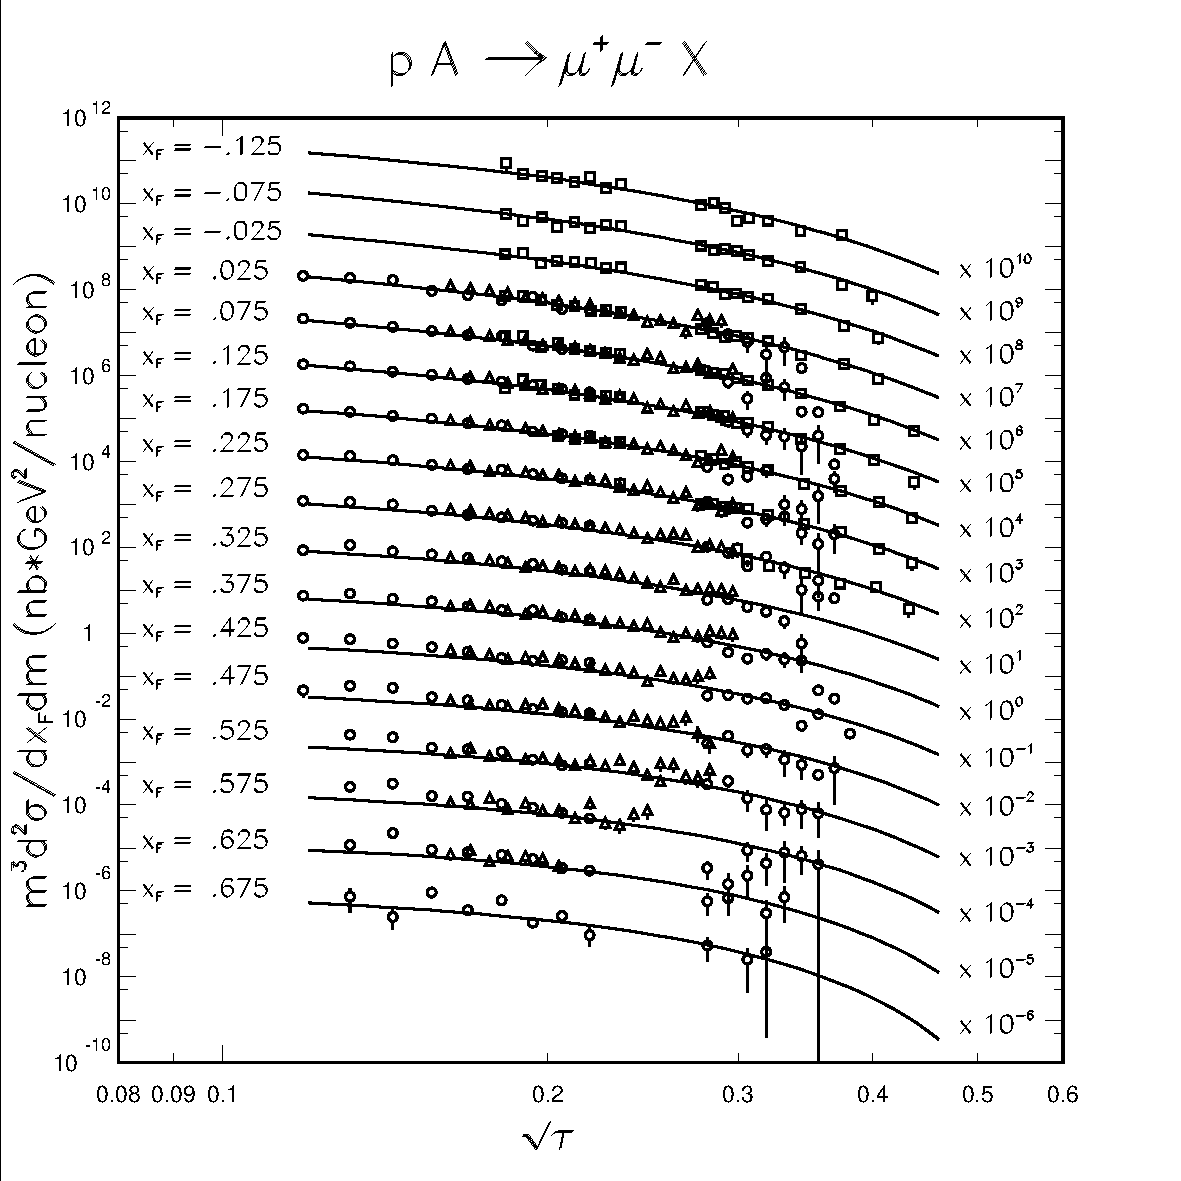
\includegraphics[width=0.8\linewidth]{DY_scaling}
	\caption{Compilation of data on Drell-Yan process, and compared with NLO calculations,
		taken from Ref.~\cite{mcgaughey1999}.}
	\label{fig:DY_scaling}
\end{figure}

One of the advantages of Drell-Yan over DIS is the explicit separation of the quark
and anti-quark distributions in \cref{eq:DY_cs}. At large $x$, DIS cross section
is dominated by the valence quark distribution. On the other hand, in the region $x_1 \gg x_2$,
the valence quark in the Drell-Yan process is more likely to come from the beam
hadron, and the anti-quark is more likely to come from the target hadron. Hence,
Drell-Yan can be more sensitive to the anti-quark distribution than DIS. In
particular, the $\sigma_{pd}/2\sigma_{pp}$ Drell-Yan cross section ratio at leading order
can be approximated as
\begin{equation}
	\frac{\sigma_{pd}}{2\sigma_{pp}}\approx \frac{\sigma_{pp}+\sigma_{pn}}{2\sigma_{pp}}
	\stackrel{x_1\gg x_2}{\approx} \frac{1}{2} \left( 1+ \frac{\frac{\bar{d}\left(x_2\right)}{\bar{u}\left(x_2\right)} + \frac{d\left(x_1\right)}{4u\left(x_1\right)} }{1+\frac{d\left(x_1\right)}{4u\left(x_1\right)} \frac{\bar{d}\left(x_2\right)}{\bar{u}\left(x_2\right)} }\right).
\end{equation}
The first approximation sign indicates that nuclear correction in deuteron is assumed to be negligible~\cite{ehlers2014}.
In the limit $x_1$ is sufficiently large, $d\left(x_1\right)/u\left(x_1\right)$ is expected
to be small, and thus this ratio can be directly related to the light sea-quark
asymmetry. The Drell-Yan process has been used in several experiments to probe the sea-quarks
asymmetry, with the goal of measuring the $x$ dependence of the sea-quark asymmetry
instead of only the integral as with the Gottfried sum rule.


\section{E866/NuSea}
\label{sec:E866}
Utilizing the sensitivity of the Drell-Yan process to the sea-quark asymmetry,
the E866/NuSea experiment~\cite{towell2001} was designed to measure the $\sigma_{pd}/2\sigma_{pp}$
Drell-Yan cross section ratio over a broad range of $x$. The
experiment utilized the \SI{800}{\GeV} proton beam from the Tevatron on liquid
hydrogen and deuterium targets. The measured deuterium over hydrogen cross section
ratio from E866/NuSea is shown in \cref{fig:e866_result}. At low $x$, the ratio is consistent
with a symmetric sea, and the asymmetry becomes larger as $x$ increases, as expected from
the model predictions. However, at $x_2>0.25$ the cross section ratios
drop below unity, suggesting that the $\bar{d}/\bar{u}$
ratio drop below 1, which could not be explained by models at the time.
Due to the large uncertainty on the data points at large $x_2$, a new
experiment was needed to explore sea quark asymmetry the high $x$ region with better
accuracy.
\begin{figure}[htbp!]
	\centering
	\begin{subfigure}{0.48\linewidth}
		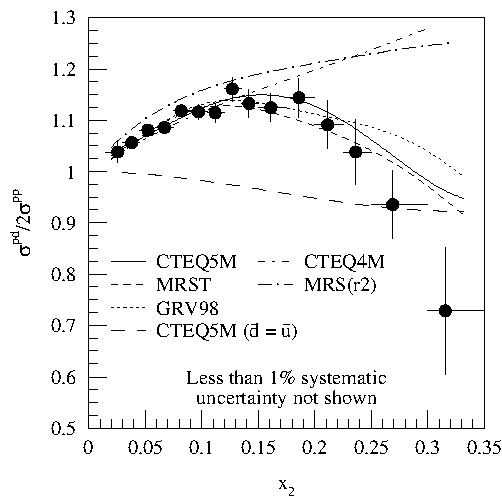
\includegraphics[width=\linewidth]{e866_csr}
		\caption{$\sigma_{pd}/2\sigma_{pp}$ Drell-Yan cross section ratio.}
		\label{subfig:e866_csr}
	\end{subfigure}
	\begin{subfigure}{0.48\linewidth}
		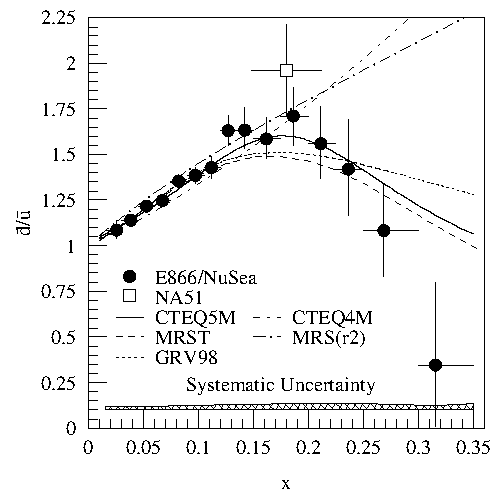
\includegraphics[width=\linewidth]{e866_dbarubar}
		\caption{$\bar{d}/\bar{u}$ extracted from E866 result.}
		\label{subfig:e866_dbarubar}
	\end{subfigure}
	\caption{The E866 result taken from Ref.~\cite{towell2001}.}
	\label{fig:e866_result}
\end{figure}

\section{Origin of the \texorpdfstring{$\bar{d}/\bar{u}$}{dbar/ubar} Asymmetry }
After the result from NMC and other DIS experiments indicating the violation of the Gottfried sum rule,
various models have been proposed to explain the $\bar{d}/\bar{u}$ asymmetry. One of the early proposal
is by Field and Feynman~\cite{field1977}. They suggested that the Pauli blocking effect
could suppress the production of $u\bar{u}$ pairs relative to  $d\bar{d}$ due to the presence of two
valence $u$ quarks and only one valence $d$ quark in the proton.
It was later shown that the effect by Pauli blocking would be small and
may actually have an opposite effect~\cite{steffens1997}. Since the contribution from gluon splitting to the
sea quarks is flavor-blind and the mass of $u$ and $d$ quarks are roughly equal, the asymmetry in the
light sea-quarks must originate from a non-perturbative mechanism. Some of the models will be presented
in this section.

\subsection{Meson Cloud Model}
Some of the early models attribute the asymmetry to the existence of a ``pion cloud'' in the proton.
In the meson cloud model~\cite{kumano1998,speth2002} the proton wave function is written as a sum of meson-baryon states
\begin{equation}
	\ket{p} = \sqrt{Z}\ket{p}_{\mathrm{bare}} + \sum_{MB}\int \dd{y} \dd[2]{\vec{k}_\perp} \phi_{BM} \left(y, k^2_\perp\right)\ket{M\left(y, \vec{k}_\perp\right);B\left(1-y, -\vec{k}_\perp\right)}
\end{equation}
where $\phi_{BM}$ is the amplitude to find a physical nucleon in a state consisting of a virtual
meson $M$ and virtual baryon $B$ with longitudinal momentum fractions $y$ and $1-y$ and transverse momenta
$\vec{k}_\perp$ and $-\vec{k}_\perp$ respectively. $Z$ is the standard wave function normalization factor
and can be interpreted as the probability of finding a bare proton, which only contains a symmetric sea and the valence quarks.

The main hypothesis is that the exchanged photon in the DIS process can interact with the partons in the
virtual meson or the virtual
baryon. Therefore, the PDF can be related to the PDFs of either the stuck meson or stuck baryon.
\begin{equation}
	f_{i/N}\left(x\right) = f_{i/N}^{\mathrm{bare}}\left(x\right) +  \int^1_x f_{MB/N}\left(y\right) f_{i/M}\left(\frac{x}{y}\right) \frac{\dd{y}}{y} + \int^1_x f_{BM/N}\left(y\right) f_{i/B}\left(\frac{x}{y}\right) \frac{\dd{y}}{y},
\end{equation}
where $f_{MB/N}$ and $f_{BM/N}$ are the splitting function, related to $\phi_{BM}$, and $f_{MB/N}(y)=f_{BM/N}(1-y)$.
If we restrict to $\pi N$ and $\pi\Delta$ states, and using isospin symmetry,
\begin{align}
	f_{\pi^+n/p}=\frac{2}{3} f_{\pi N}                                       & , ~f_{\pi^0 p/p}=\frac{1}{3} f_{\pi N},                                         \\
	f_{\pi^-\Delta^{++}/p}=\frac{1}{2} f_{\pi \Delta}, ~f_{\pi^0 \Delta^+/p} & =\frac{1}{3} f_{\pi \Delta},  ~f_{\pi^+ \Delta^0/p}=\frac{1}{6} f_{\pi \Delta}.
\end{align}
The light sea-quark distributions in the proton are given by
\begin{align}
	\bar{d}(x) & = \left(\frac{5}{6}f_{\pi N} + \frac{1}{3}f_{\pi \Delta}\right)\otimes q^v_\pi + S(x) \\
	\bar{u}(x) & = \left(\frac{1}{6}f_{\pi N} + \frac{2}{3}f_{\pi \Delta}\right)\otimes q^v_\pi + S(x)
	\label{eq:pion_dbub}
\end{align}
where $f\otimes q\equiv \int^1_x \frac{dy}{y}f(y)q\left(\frac{x}{y}\right)$, $q^v_\pi$ is the valence
quark distribution in pions, and $S(x)$ is the flavor symmetric contributions.
The asymmetry in the proton sea arises because of the dominance of the $\pi^+$ among the $\pi N$ states.
However, the effect is slightly reduced by the $\pi\Delta$ configurations, which favors $\bar{u}$ over $\bar{d}$.
As the $\Delta$ baryon is heavier than the proton, the $\pi\Delta$ configurations should be less important than
the $\pi N$ configurations.
If we took the difference $\bar{d}-\bar{u}$, the flavor symmetric contribution $S(x)$ would cancel out.
\Cref{fig:pion_cloud}
shows the predicted $\bar{d}-\bar{u}$ from the meson cloud model, taken from Ref.~\cite{alberg2022}.
\begin{figure}
	\centering
	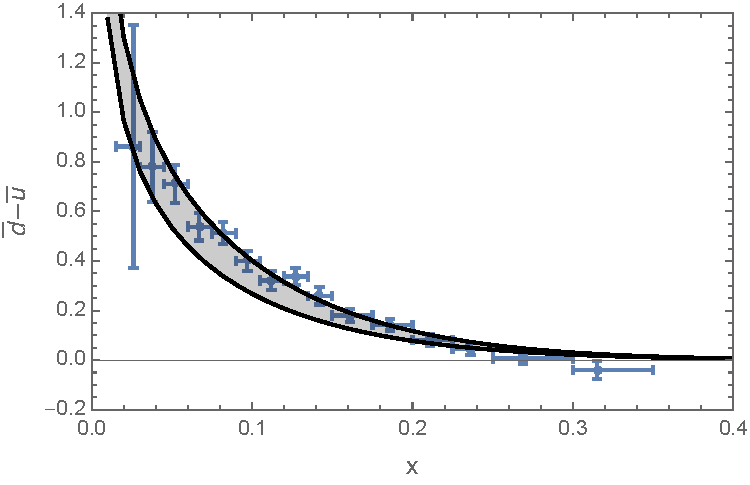
\includegraphics[width=0.6\linewidth]{rediff}
	\caption{The predicted $\bar{d}-\bar{u}$ from the meson cloud model and compared with the E866 results (blue symbol), taken from Ref.~\cite{alberg2022}.}
	\label{fig:pion_cloud}
\end{figure}

\subsection{Chiral Quark Model}
Similar to the meson cloud model, the chiral quark model~\cite{li1998} attributes the sea quarks to
the presence of Goldstone bosons in the nucleon. However, the Goldstone bosons in chiral quark model
are emitted from the valence quarks. The quark helicity would also be modified by the emission of a
spin-zero meson in P-wave, as indicated by the subscripts.
\begin{equation}
	q_{\pm} \rightarrow GB + q^\prime_\mp \rightarrow \left(q q^\prime\right)_0 q_{\mp}^\prime.
\end{equation}
For example, after one emission, the $u$ quark wavefuction would have the following components
\begin{equation}
	\Psi\left(u\right) \sim \left[d\pi^+ + s K^+ + u \left(\frac{\pi^0}{\sqrt{2}} + \frac{\eta}{\sqrt{6}}\right)\right],
\end{equation}
which can be expressed in terms of the quark contents by using $\pi^+ = u\bar{d}$ and $K^+ = u\bar{s}$. etc.
The probability of the transitions is given by squaring the wavefunction, and if
\begin{equation}
	Prob\left[ u_+ \rightarrow \pi^+d_-\right] \equiv a,
\end{equation}
and using charge asymmetry to determine the $d$ quark wavefucntion, the number of antiquark after one emission
by the initial $(2u+d)$ valence quarks in the proton is given by
\begin{equation}
	\begin{aligned}
		\bar{u} \equiv \int^1_0 \dd{x}\bar{u}(x) & = 2\cross\frac{4}{9}a +a+\frac{1}{9}a = 2a,                         \\
		\bar{d} \equiv \int^1_0 \dd{x}\bar{d}(x) & = 2\cross\left(a+\frac{1}{9}a\right) + \frac{4}{9}a = \frac{8}{3}a.
	\end{aligned}
\end{equation}
Therefore the model predicts a light sea-quark asymmetry $\bar{d}-\bar{u} =\frac{2}{3}a $.
Unlike the meson cloud model, the Goldstone boson in the chiral quark model are emitted
by the valance quarks, which only carry a fraction of the total hadron's momentum.
Therefore the boson in the chiral quark model would necessarily carry a smaller momentum than
it would in the meson cloud model, and the sea-quark distributions would peak at a lower value of $x$ \cite{szczurek1996,peng1998}.



\subsection{Statistical Model}
In the statistical model~\cite{bourrely2015}, the nucleon is viewed as a gas of massless partons in equilibrium in
a finite volume. And the parton distributions at the initial scale would then be proportional to
\begin{equation}
	\left[ \exp\left[\left(x-X_{0p}\right)/\bar{x}\right] \pm 1 \right]^{-1},
\end{equation}
where the plus sign for the quarks and antiquarks corresponds to a Fermi-Dirac distribution and
the minus sign for gluons corresponds to a Bose-Einstein distribution. The constant $X_{0p}$
plays the role of the thermodynamic potential of the parton $p$ and $\bar{x}$ is the universal
temperature.

In this model, the potential of a quark $q_i^h$ with helicity $h$ has an opposite sign to that of the
potential of the corresponding antiquark $q_i^{-h}$ with helicity $-h$
\begin{equation}
	X_{0q}^h = -X_{0\bar{q}}^{-h}.
	\label{eq:stat_potential}
\end{equation}
Since there are more $u$ quarks than $d$ quarks in the proton, one would expect
\begin{equation}
	X_{0u}^+ + X_{0u}^- > X_{0d}^+ + X_{0d}^-,
\end{equation}
and combining with \cref{eq:stat_potential}, one would expect $\bar{d} > \bar{u}$ in the proton.
And this is shown in \cref{fig:stat_dbub}.
\begin{figure}[h]
	\centering
	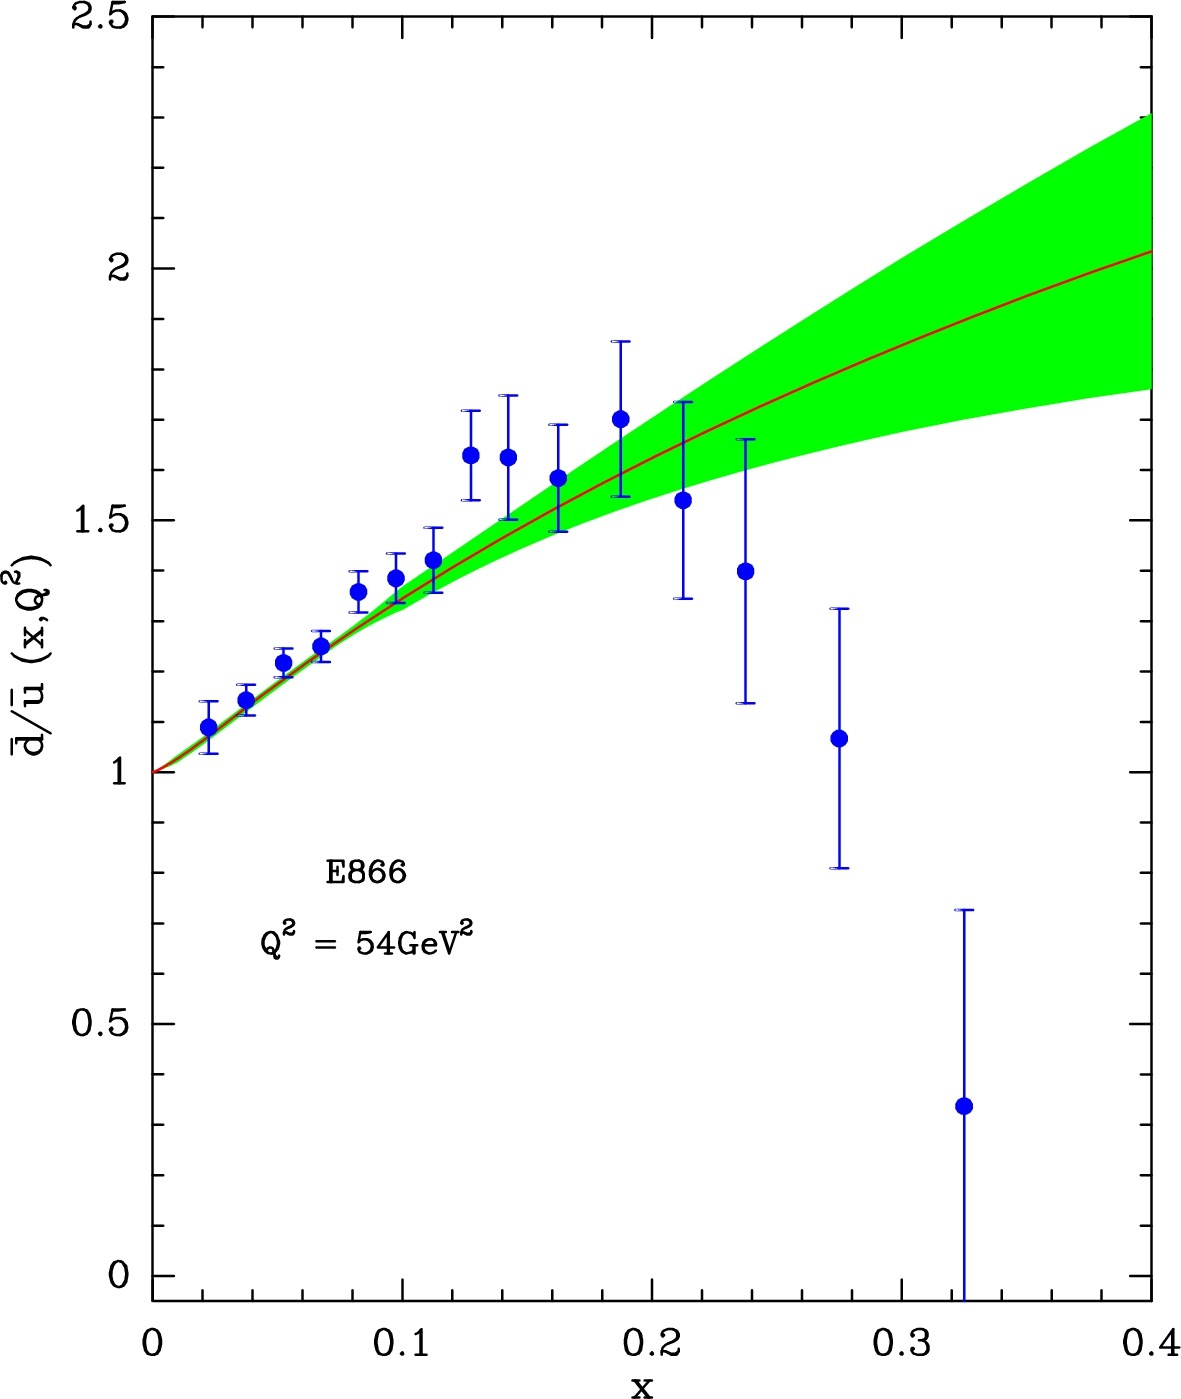
\includegraphics[width=0.5\linewidth]{statistical_model}
	\caption{The extracted light sea-quark asymmetry from the statistical model and compared with E866, taken
		from Ref.~\cite{soffer2019}.}
	\label{fig:stat_dbub}
\end{figure}


\subsection{Five-quark Intrinsic Sea Model}
In the 1980s, Brodsky, Hoyer, Peterson and Sakai (BHPS)~\cite{brodsky1980} proposed
the possible existence of a significant $\ket{uudc\bar{c}}$ five-quark Fock state component
in the proton in order to explain the larger than expected charmed hadrons production rate.

For a $\ket{uudQ\bar{Q}}$ proton Fock state, the probability for quark $i$ to carry a momentum
fraction $x_i$ is given by
\begin{equation}
	P\left(x_1,\cdots,x_2\right)=N_5 \delta\left(1-\sum^5_{i=1}x_i\right)\left[m_p^2-\sum^5_{i=1}\frac{m_i^2}{x_i}\right]^{-2},
\end{equation}
where the delta function ensures momentum conservation. $N_5$ is the normalization factor,
and $m_i$ is the mass of quark $i$.

Since the BHPS model also predicts the probability for the $\ket{uudQ\bar{Q}}$ configuration to
be proportional to $1/m^2_Q$, where $m_Q$ is the mass of quark $Q$, the intrinsic sea can have important
contribution to the light sea-quarks. In Refs.~\cite{chang2011,chang2011a}, the BHPS model
was extended to the light quark sector. In this model, the $\bar{u}$ and $\bar{d}$ are predicted
to  have the same $x$ dependence if one assumes $m_u=m_d$. The only source of asymmetry
are the probabilities of the $\ket{uudd\bar{d}}$ and $\ket{uudu\bar{u}}$ configurations,
which are not known from the BHPS model, and remain to be determined from experiments.
Nevertheless, the $x$ dependence of the $\bar{d}-\bar{u}$ asymmetry can be obtained from the model.
\Cref{fig:five_quark} shows the comparison of the $\bar{d}-\bar{u}$ data from E866 with calculation
based on BHPS model, with normalization fixed by the measured asymmetry. At the initial scale,
the sea-quark distribution exhibit a valence like behavior. As the scale increases, the distribution
becomes softer.
\begin{figure}[hb!]
	\centering
	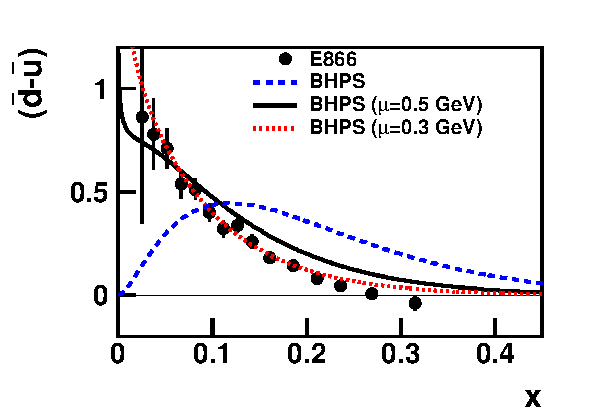
\includegraphics[width=0.6\linewidth]{fig_dbarubar}
	\caption{Comparison of the $\bar{d}-\bar{u}$ data with calculation based on BHPS model.
		The dashed curve corresponds the distribution at initial scale, and the solid and dotted
		curve are obtained by evolving to $Q^2=\SI{54}{\GeV\squared}$ assuming different initial scale $\mu$.
		Taken from Ref.~\cite{chang2011}. }
	\label{fig:five_quark}
\end{figure}

Recent global analysis from NNPDF~\cite{ball2022} and measurement from the LHCb~\cite{aaij2022}
have suggested evidence of intrinsic charm in the proton. This has led to many recent theory
development in understanding the nonperturbative charm in the proton~\cite{guzzi2023}. There are
also suggestions that SeaQuest kinematic would be ideal for testing limits on intrinsic charm~\cite{vogt2021}.

\subsection{Lattice QCD}
\label{subsec:lattice}
Lattice QCD calculations of the $\bar{d} - \bar{u}$ based on the Large Momentum Effective
theory (LaMET)~\cite{ji2021,constantinou2021} have become available recently by two different groups,
LP3~\cite{chen2018} and ETMC~\cite{alexandrou2018}.
The parton distribution functions described quarks and gluons in hadrons traveling at infinite
momentum. The principle for LaMET comes from the observation that the structure of the proton is
approximately independent of its momentum so long as it is much larger than the strong interaction
scale or its mass. Therefore the partonic structure can be calculated for a proton with
moderately-large momentum and taking the limit of the proton momentum to infinity.

\begin{figure}[h!]
	\centering
	\begin{subfigure}{0.45\linewidth}
		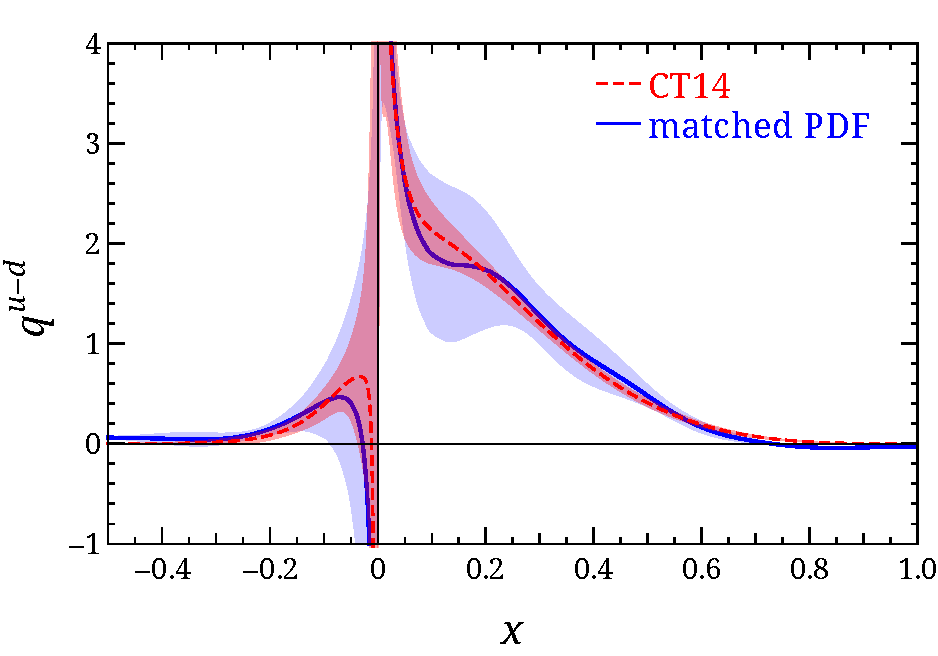
\includegraphics[width=\linewidth]{LP3-PDF-CT14}
	\end{subfigure}
	\begin{subfigure}{0.45\linewidth}
		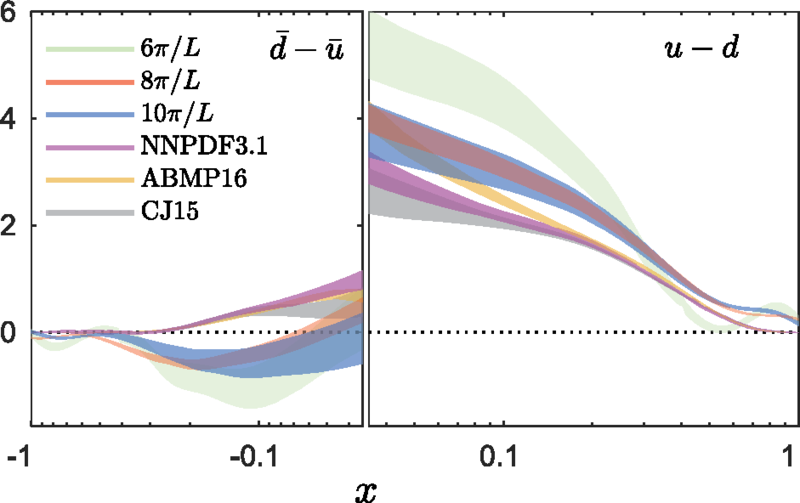
\includegraphics[width=\linewidth]{alexandrou2018}
	\end{subfigure}
	\caption{The calculated isovector PDF from the LP3 collaboration (left)~\cite{chen2018}
		and ETMC (right)~\cite{alexandrou2018}.
		The negative $x$ region denote $\bar{d}-\bar{u}$ at $\left|x\right|$.}
	\label{fig:lamet}
\end{figure}
LaMET are typically used to calculate flavor non-singlet quantities such as $u-d$ and $\bar{d}-\bar{u}$,
as the disconnected diagram would cancel out in the calculation.
\Cref{fig:lamet} shows the results using LaMET from two different groups and are compared with
different global PDF extractions. While the result by the LP3 collaboration
is in good agreement with CT14, the result from the ETMC group differs from the PDFs,
especially in the antiquark region.

\chapter{Charmonium Production}
\label{ch:jpsi}
Another process for probing the nucleon structure is the charmonium production~\cite{peng1995,chang2020}.
Unlike DIS and Drell-Yan, the charmonium production involves strong interaction already
at the leading-order. Therefore it can be used to probe the gluon structure, which 
the DIS or Drell-Yan processes are less sensitive to, and the quark and anti-quark structures.
At leading order, charmonium production involves two sub-processes, gluon fusion and
quark-antiquark annihilation into a gluon, as illustrated in \cref{fig:charmonium}.

The simultaneous measurement of charmonium production and Drell-Yan process, two very different
processes, can provide complementary information on the partonic structures of the nucleon.
In particular, the $\sigma_{pd}/2\sigma_{pp}$ ratio for charmonium
production is expected to be sensitive to the ratio of the gluon distributions in the proton
and neutron, as well as the $\bar{d}/\bar{u}$ ratio in the proton.

If quark-antiquark annihilation is the dominant process for charmonium
production, the $\sigma_{pd}/2\sigma_{pp}$ ratio would provide an
independent measurement of the $\bar{d}/ \bar{u}$ flavor asymmetry in the
proton~\cite{peng1995}, complementary to the Drell-Yan process.
On the other hand, if gluon-gluon fusion is the dominant process, the
$\sigma_{pd}/2\sigma_{pp}$ ratio could probe the relative gluon content
in the proton and neutron, providing a test of the charge symmetry at the partonic level.
Violation of charge symmetry is predicted at both the hadronic~\cite{stephenson2003,opper2003}
and the partonic levels~\cite{londergan2010}. Since gluon is an iso-scalar particle,
charge symmetry requires that the gluon distributions in the proton and neutron
are identical. A measurement of the gluon contents in proton and neutron could test charge symmetry at
the partonic level~\cite{piller1996,zhu2008,lansberg2012}.

As $J/\psi$ and $\psi'$ are resonances, they show up as peaks in the dimuon mass spectrum,
and the cross section is significantly larger than the Drell-Yan cross section.
However, there are various models for calculating the quarkonium production,
which contains non-perturbative aspects of QCD.
The models usually separate the production
mechanism into two parts, the production of heavy-quark pairs and their subsequent
hadronization into quarkonium states. One of the early approaches is the Color
Evaporation Model (CEM)~\cite{einhorn1975,bodwin1995}. The heavy-quark
pairs production is expanded in terms of the strong coupling constant $\alpha_s$
and is calculated with perturbative QCD (pQCD). CEM then assumes a constant
probability $F$ for the $c\bar{c}$ pairs to hadronize into a specific quarkonium
state and this probability is independent of the kinematics or the production
subprocess. The $J/\psi$ production cross section in the CEM framework can be
expressed as
\begin{equation}
	\begin{split}
		\left.\frac{d\sigma}{dx_F}\right|_{J/\psi} & = F \sum_{i,j = q,\bar{q},G}\int^{2m_D}_{2m_c} dM_{c\bar{c}}  \frac{2M_{c\bar{c}}}{s\sqrt{x_F^2+4M_{c\bar{c}}^2/s}}                                 \\
		                                           & \cross f_{i/A}\left(x_1,\mu_F\right)f_{j/B}\left(x_2,\mu_F\right)\sigma\left[ij\rightarrow c\bar{c}X\right]\left(x_1P_A,x_2P_B,\mu_F,\mu_R \right),
	\end{split}
\end{equation}
where $i$, $j$ denote the type of interacting partons.
\begin{figure}[htpb!]
	\centering
	\begin{subfigure}[c]{0.4\linewidth}
		\begin{subfigure}[c]{\linewidth}
			\begin{tikzpicture}
	\tikzstyle{every node}=[font=\large]
	\begin{feynman}
		\vertex  (a1);
		\vertex [right= of a1, blob] (a2) {};
		\vertex [right= 2cm of a2] (a3) ;
		\vertex [below= 3cm of a1] (b1);
		\vertex [below= 3cm of a2,blob] (b2) {};
		\vertex[below= 3cm of a3] (b3);
		\vertex  at ($(b2) + (1cm , +1.5cm)$) [dot] (d);
		\vertex [right= 2cm of d] (d1);
		\vertex at ($(d1) + (1cm , +1.2cm)$) (c1) {$c$};
		\vertex at ($(d1) + (1cm , -1.2cm)$) (c2) {$\bar{c}$};
		\diagram*{
		(a1) --[fermion](a2),
		(a2) --[double distance=4pt, thick](a3),
		(b1) --[fermion](b2),
		(b2) --[double distance=4pt, thick](b3),
		(b2) --[gluon, edge label'=$g$] (d),
		(a2) --[gluon, edge label=$g$](d),
		(d) --[gluon](d1),
		(c2) --[fermion] (d1);
		(d1) --[fermion] (c1);
		};
	\end{feynman}
\end{tikzpicture}

		\end{subfigure}
		\begin{subfigure}[c]{\linewidth}
			\begin{tikzpicture}
	\tikzstyle{every node}=[font=\large]
	\begin{feynman}
		\vertex  (a1);
		\vertex [right= of a1, blob] (a2) {};
		\vertex [right= 2cm of a2] (a3) ;
		\vertex [below= 3cm of a1] (b1);
		\vertex [below= 3cm of a2,blob] (b2) {};
		\vertex [below= 3cm of a3] (b3);
		\vertex  at ($(b2) + (1.5cm , +1cm)$) [dot] (d);
		\vertex [above= 1cm of d] (d1);
		\vertex [right= 2.25cm of d1] (c1) {$c$};
		\vertex [right= 2.25cm of d] (c2) {$\bar{c}$};
		\diagram*{
		(a1) --[fermion](a2),
		(a2) --[double distance=4pt, thick](a3),
		(b1) --[fermion](b2),
		(b2) --[double distance=4pt, thick](b3),
		(b2) --[gluon, edge label=$g$] (d),

		(a2) --[gluon, edge label'=$g$](d1),
		(d) --[fermion](d1),
		(d1) --[fermion] (c1);
		(c2) --[fermion] (d);
		};
	\end{feynman}
\end{tikzpicture}

		\end{subfigure}
		\caption{Gluon fusion\label{subfig:gluon}.}
	\end{subfigure}
	\quad
	\begin{subfigure}[c]{0.4\linewidth}
		\begin{tikzpicture}
	\tikzstyle{every node}=[font=\large]
	\begin{feynman}
		\vertex  (a1);
		\vertex [right= of a1, blob] (a2) {};
		\vertex [right= 2cm of a2] (a3) ;
		\vertex [below= 3cm of a1] (b1);
		\vertex [below= 3cm of a2,blob] (b2) {};
		\vertex[below= 3cm of a3] (b3);
		\vertex  at ($(b2) + (1cm , +1.5cm)$) [dot] (d);
		\vertex [right= 2cm of d] (d1);
		\vertex at ($(d1) + (1cm , +1.2cm)$) (c1) {$c$};
		\vertex at ($(d1) + (1cm , -1.2cm)$) (c2) {$\bar{c}$};
		\diagram*{
		(a1) --[fermion](a2),
		(a2) --[double distance=4pt, thick](a3),
		(b1) --[fermion](b2),
		(b2) --[double distance=4pt, thick](b3),
		(b2) --[anti fermion, edge label'=$\bar{q}$] (d),
		(a2) --[fermion, edge label=$q$](d),
		(d) --[gluon](d1),
		(c2) --[fermion] (d1);
		(d1) --[fermion] (c1);
		};
	\end{feynman}
\end{tikzpicture}

		\caption{Quark-antiquark annihilation.\label{subfig:qqbar}}
	\end{subfigure}
	\caption{The Feynman diagrams for $c\bar{c}$ pair production.}
	\label{fig:charmonium}
\end{figure}
While proton induced $J/\psi$ production is often dominated by gluon fusion
process~\cite{vogt1999}, the relative importance of gluon fusion
and quark-antiquark annihilation is a strong function of hadron-hadron center-of-mass energy $\sqrt{s}$
and $x_F=2P_L/\sqrt{s}$, where $P_L$ is the longitudinal momentum of the $J/\psi$ meson in the
hadron-hadron center-of-mass frame.
The NA51 collaboration reported a measurement of the $p+p$ and $p+d$ cross sections
for the charmonium at \SI{450}{\GeV} at a single value of rapidity ($x_F\sim 0$)~\cite{abreu1998}.
The SeaQuest measurement covers a broader kinematic range of $0.5<x_F<0.9$ at a lower beam energy
of \SI{120}{\GeV}.
The calculated cross section for $J/\psi$ production in $p+p$ at \SI{120}{\GeV} using
CEM is shown in \cref{fig:cem_cs}.
At our beam energy, the quark-antiquark annihilation would be more important than gluon fusion at large $x_F$, where
the SeaQuest experiment has better coverage.
\begin{figure}[h!]
	\centering
	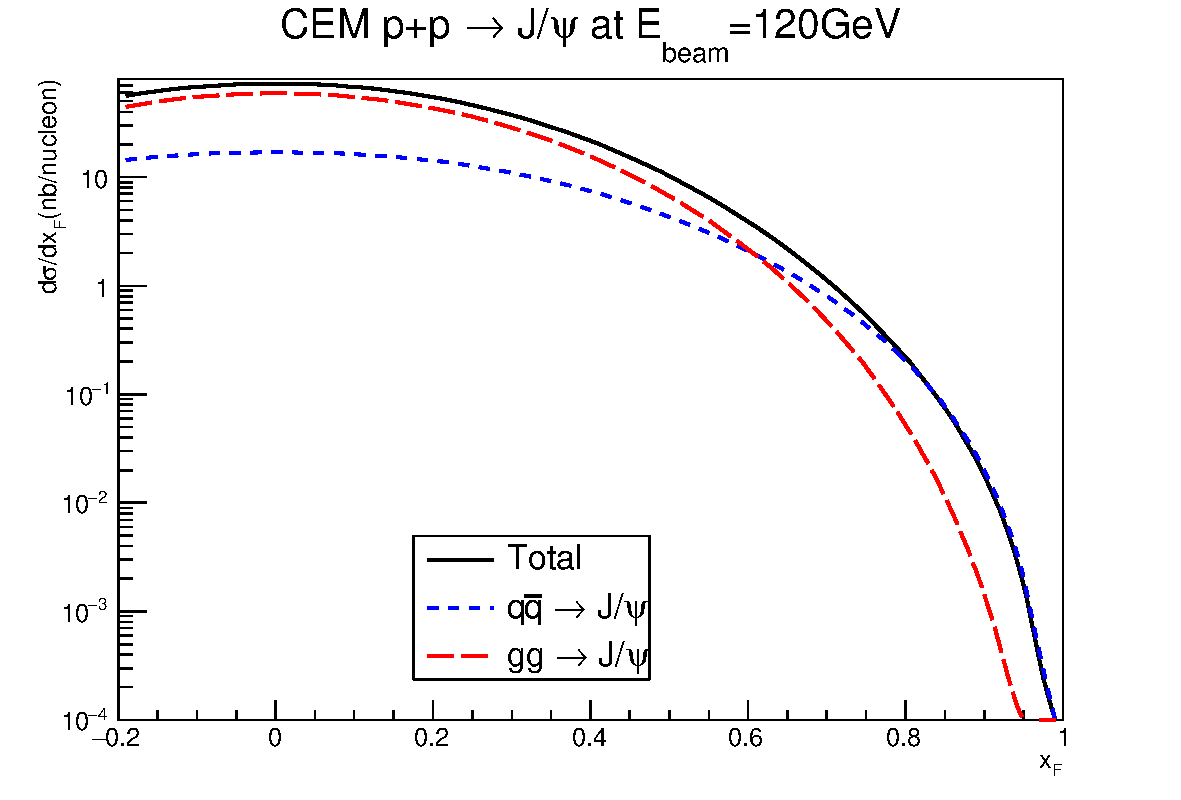
\includegraphics[width=0.45\linewidth]{pp_norm_cs_NLO_pp}
	\caption{Calculated cross section for $J/\psi$ production using the CEM model with the CT14NLO PDF.
		The CEM code is obtained from Ref.~\cite{mangano1993}.}
	\label{fig:cem_cs}
\end{figure}

Another theoretical model for quarkonium production is the non-relativistic
QCD (NRQCD) \cite{bodwin1995}. Unlike CEM, the probability of
hadronization depends on the color and spin state of the $c\bar{c}$ pairs and
is described by various long-distance matrix elements (LDMEs). The quarkonium
production cross section in this framework is given as
\begin{equation}
	\begin{split}
		\frac{d\sigma^H}{dx_F} & =\sum_{i,j = q,\bar{q},G}\int^1_0 dx_1 dx_2 \delta(x_F-x_1+x_2)                                                                                        \\
		                       & \cross f_{i/A}\left(x_1,\mu_F\right)f_{j/B}\left(x_2,\mu_F\right)\hat{\sigma}\left[ij\rightarrow H\right]\left(x_1P_A,x_2P_B,\mu_F,\mu_R , m_c\right),
	\end{split}
\end{equation}
\begin{equation}
	\hat{\sigma}\left[ij\rightarrow H\right]= \sum_n C^{ij}_{c\bar{c}\left[n\right]}\left(x_1P_A,x_2P_B,\mu_F,\mu_R , m_c\right)\expval{O^H_n}.
\end{equation}
The $c\bar{c}$ pairs are produced in state $n={^{2S+1}L_J^{\left[a\right]}}$ with definite spin $S$,
orbital angular momentum $L$, total angular momentum $J$, and color state $a=1,8$.
The coefficient $C^{ij}_{c\bar{c}\left[n\right]}$ describes the production of $c\bar{c}$ pair in state $n$,
from partons $i$ and $j$ and is calculated perturbatively in powers of $\alpha_s$ using pQCD.
The LDME $\expval{O^H_n}$ accounts for the hardronization probability for a specfic $c\bar{c}$ state $n$ into the
charmonium state $H$.
This formalaism suggests that the $c\bar{c}$ pairs can be produced in color-octet state,
then evlove into physical color-singlet quarkonia by nonperturbative emission of soft gluons.

The LDMEs discribe the hadronization process,
and are assumed to be universal and independent of beam or target hadrons and the energy scale.
As the LDMEs describe the non-pertubative interactions,
they cannot be calculated using pQCD, and have to be extracted from models or experiments.
For example, the color-singlet LDMEs are typically estmated using the potential model~\cite{eichten1995}.
Using the potential model, the wavefunction of the heavy quark pair can be calculated, 
and the color-singlet LDMEs can be estimated from the wavefunction at the origin
\begin{equation}
	\begin{split}
		\expval{O^{\psi}\left[^3S_1^{\left[1\right]}\right]} &= \frac{3N_c}{2\pi} \left| R_{\psi}\left(0\right)\right|^2,\\
		\expval{O^{\chi_{cJ}}\left[^3P_J^{\left[1\right]}\right]} &= \frac{3}{4\pi}\left(2J+1\right) \left| R'_{\chi_{cJ}}\left(0\right)\right|^2.
	\end{split}
\end{equation}
And the potential model gives $\left|R_{J/\psi}\left(0\right)\right|^2=\SI{0.81}{\GeV^3}$,
$\left|R_{\psi'}\left(0\right)\right|^2=\SI{0.53}{\GeV^3}$, and $\left|R'_{\chi_{cJ}}\left(0\right)\right|^2=\SI{0.075}{\GeV^5}$.
The other LDMEs are typically obtained by fitting to data.
Some existing LDMEs for direct $J/\psi$ and $\psi'$ productions are tabulated in \cref{tab:LDMEs}.
The values of some LDMEs from different groups are very different, in some cases, even the signs are different.
This is partly due to the choice of data sets used in their global fits. The
SeaQuest experiment can provide additonal constraints on these LDMEs. Some
existing data are shown in \cref{fig:charm_cs}.
Unlike most previous fixed-target charmonium experiments, which utilized nuclear
targets, SeaQuest have both hydrogen and deuterium targets.
Studying the charmonium production in $p+p$ and $p+d$ would allow the extraction
of the LDMEs with little, if any, model dependence from nuclear effects.

\begin{table}[ht!]
	\centering
	\caption{The NRQCD LDMEs for $J/\psi$ and $\psi'$ from different groups.}
	\label{tab:LDMEs}
	\begin{adjustbox}{width=1.03\textwidth, center=\textwidth}
		\begin{tabular}{c|ccccc}
	\hline
	                                                            & Bodwin et al~\cite{bodwin2016} & Butenschoen et al~\cite{butenschoen2011,butenschoen2023} & Chao et al~\cite{chao2012} & Gong et al~\cite{gong2013} & Feng et al~\cite{feng2019} \\ \hline
	$\expval{ O^{J/\psi}[^3S_1^{\left[1\right]}]}$ (\unit{\GeV^3})        & \num{1.32}                     & \num{1.32}                                               & \num{1.16}                 & \num{1.16}                 & \num{1.16}                 \\ \hline
	$\expval{ O^{J/\psi}[^1S_0^{\left[8\right]}]}$ (\unit{10^{-2}\GeV^3}) & \num{-0.713\pm0.364}           & \num{3.04\pm0.35}                                        & \num{8.9\pm0.98}           & \num{9.7\pm0.9}            & \num{5.66\pm0.47}          \\ \hline
	$\expval{ O^{J/\psi}[^3S_1^{\left[8\right]}]}$ (\unit{10^{-2}\GeV^3}) & \num{11.0\pm1.4}               & \num{0.168\pm0.046}                                      & \num{0.30\pm0.12}          & \num{-0.46\pm0.13}         & \num{0.177\pm0.058}        \\ \hline
	$\expval{ O^{J/\psi}[^3P_0^{\left[8\right]}]}$ (\unit{10^{-2}\GeV^5}) & \num{0.702\pm0.340}            & \num{-0.908\pm0.161}                                     & \num{1.26\pm0.50}          & \num{-2.14\pm0.56}         & \num{0.770\pm0.230}        \\ \hline \hline
	$\expval{ O^{\psi'}[^3S_1^{\left[1\right]}]}$ (\unit{\GeV^3})         & \num{0.76}                     & \num{0.76}                                               & ---                        & \num{0.758}                & ---                        \\ \hline
	$\expval{ O^{\psi'}[^1S_0^{\left[8\right]}]}$ (\unit{10^{-2}\GeV^3})  & \num{-0.157\pm0.280}           & \num{0.0958\pm0.0129}                                    & ---                        & \num{-0.012\pm0.869}       & ---                        \\ \hline
	$\expval{ O^{\psi'}[^3S_1^{\left[8\right]}]}$ (\unit{10^{-2}\GeV^3})  & \num{3.14\pm0.79}              & \num{0.149\pm0.001}                                      & ---                        & \num{0.34\pm0.12}          & ---                        \\ \hline
	$\expval{ O^{\psi'}[^3P_0^{\left[8\right]}]}$ (\unit{10^{-2}\GeV^5})  & \num{-0.257\pm0.272}           & \num{-0.0583\pm0.0056}                                   & ---                        & \num{0.945\pm0.54}         & ---                        \\ \hline
\end{tabular}
	\end{adjustbox}
\end{table}

\begin{figure}[ht!]
	\centering
	\begin{subfigure}{0.48\linewidth}
		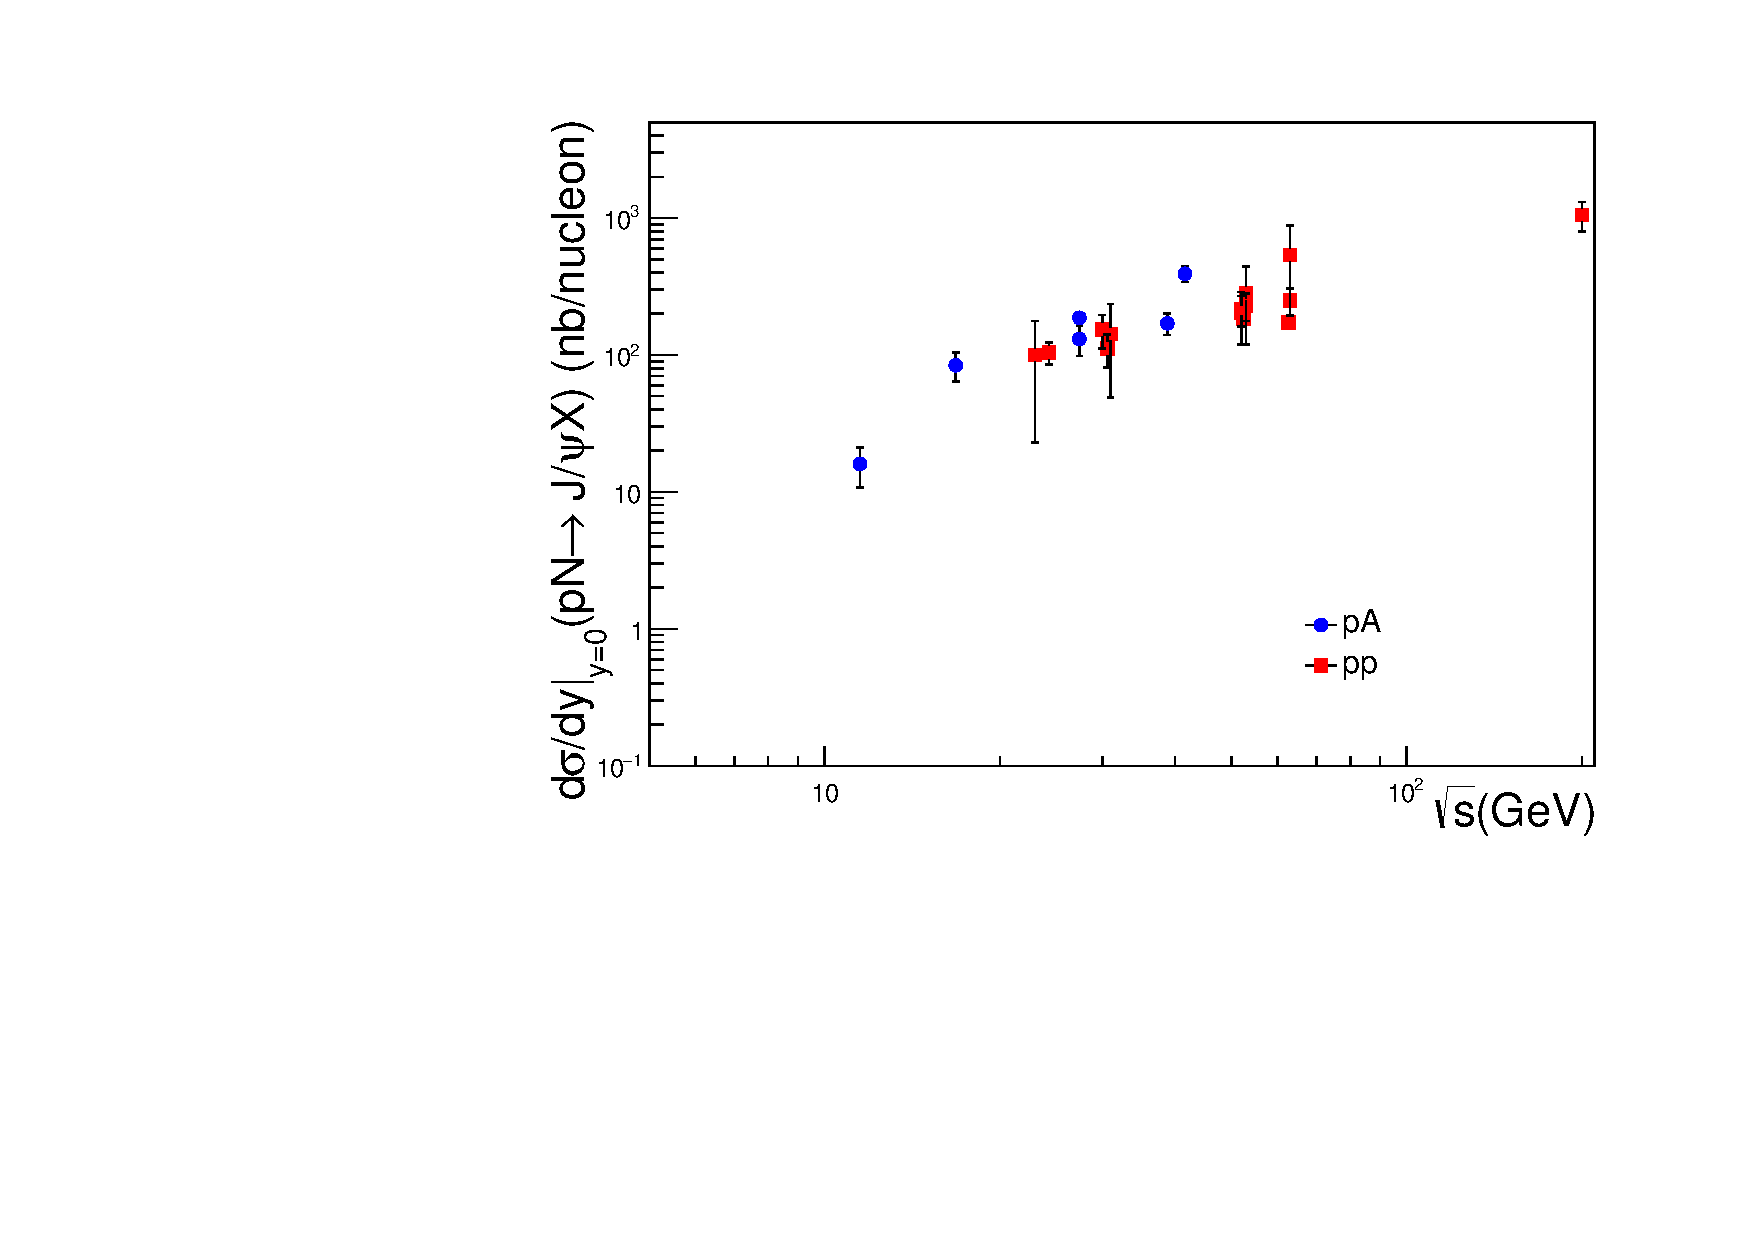
\includegraphics[width=\linewidth]{cs/sigma0}
	\end{subfigure}
	\begin{subfigure}{0.48\linewidth}
		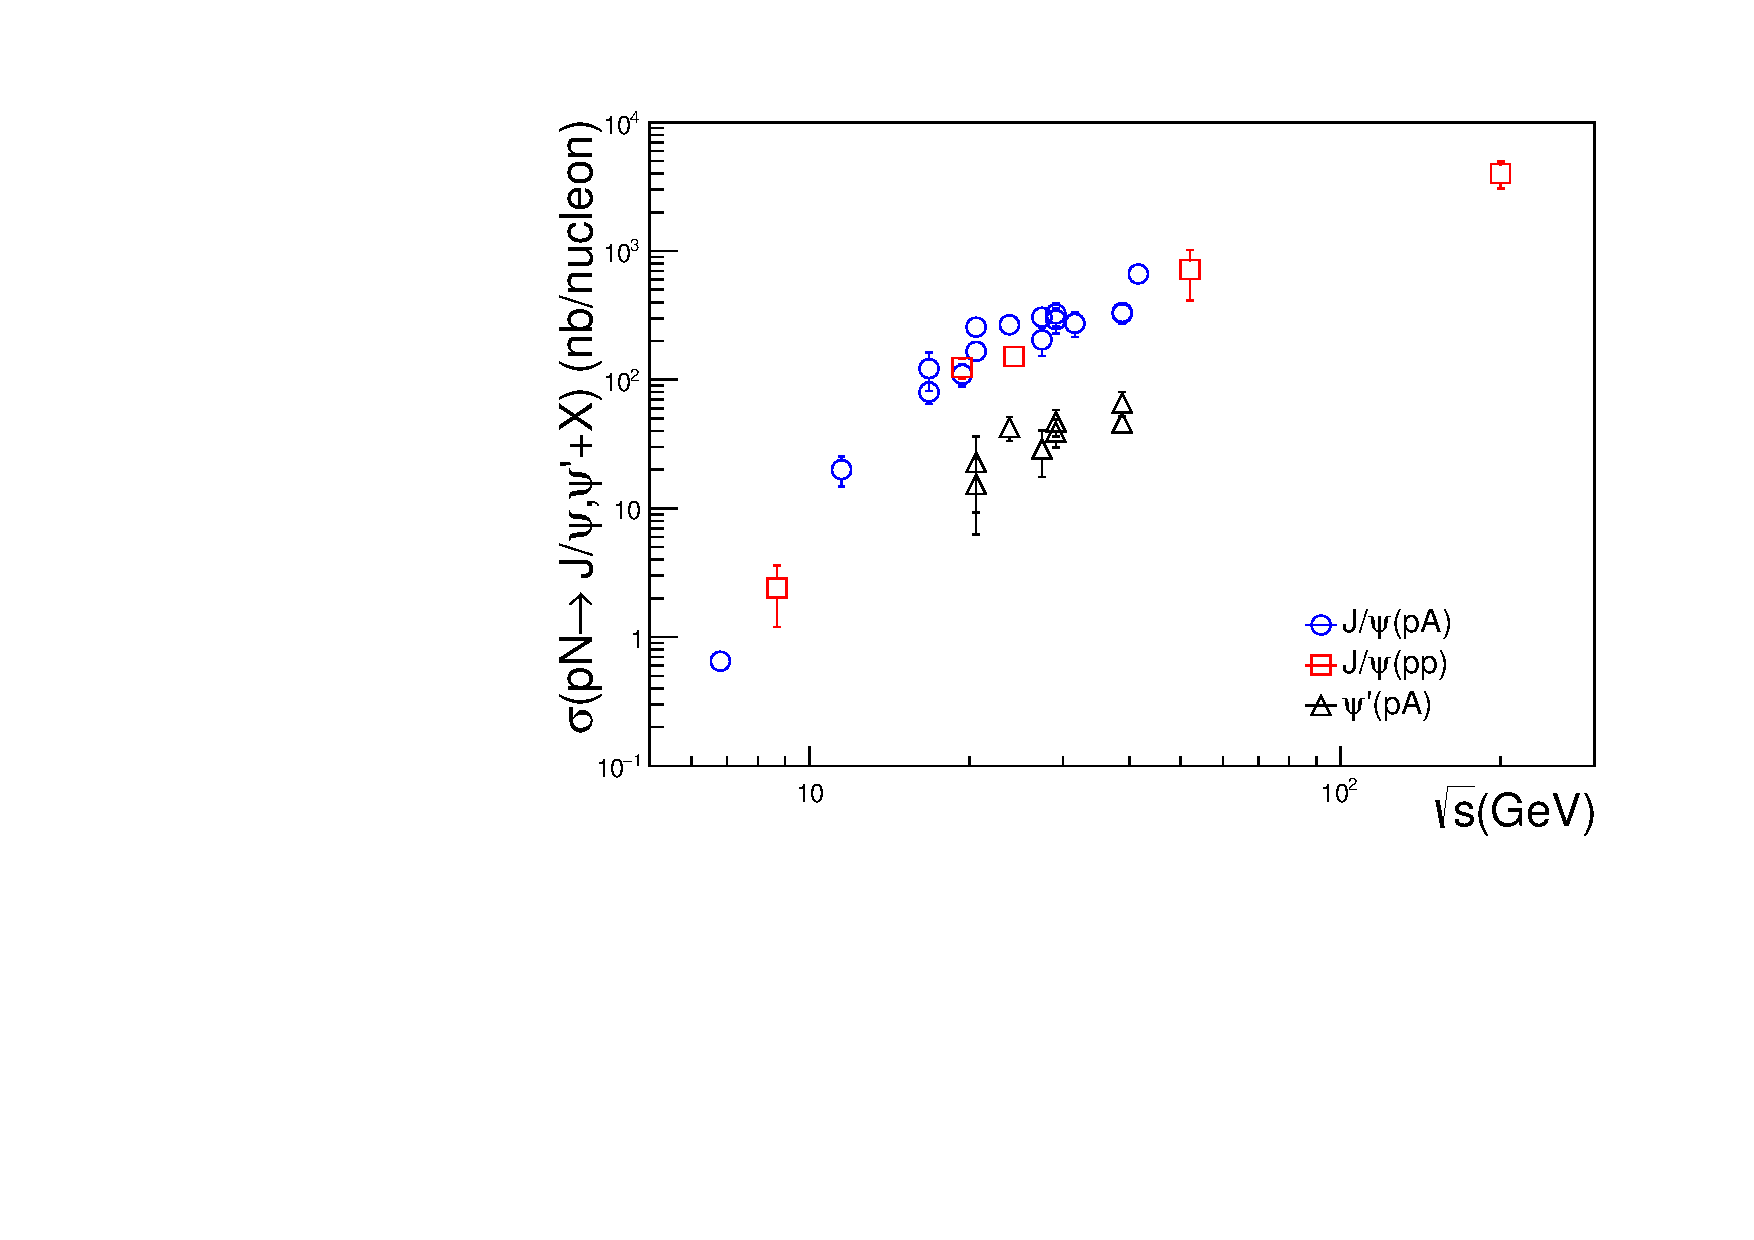
\includegraphics[width=\linewidth]{cs/sigmaTotal}
	\end{subfigure}
	\caption{The differential production cross sections at $y=0$ (left) and total
		cross section (right) in proton-proton ($pp$) and proton-nucleus ($pA$) interactions
		as a function of $\sqrt{s}$, adapted from Ref.~\cite{maltoni2006}.}
	\label{fig:charm_cs}
\end{figure}

The NRQCD calculations~\cite{chang2023a} presented in this thesis are performed using the LDMEs
from a recent global analysis of both pion- and proton-induced charmonium production data~\cite{chang2023}.
In the their analysis, only unpolarized observables were analyzed.
Therefore, the formalism can be simplified by combining the color-octet LDMEs
\begin{equation}
	\Delta^H_{[8]}=\expval{O^H\left[^1S_0^{\left[8\right]}\right]}+\frac{3}{m_c^2}\expval{O^H\left[^3P_0^{\left[8\right]}\right]}+\frac{4}{5m_c^2}\expval{O^H\left[^3P_2^{\left[8\right]}\right]}.
\end{equation}
Furthermore, the calculated cross section for $J/\psi$ also need to include the feed-down from hadronic decay
of $\psi'$ and radiative decays of three $\chi_{cJ}$ states.
Therefore the total $J/\psi$ cross section is given by
\begin{equation}
	\sigma_{J/\psi}=\sigma_{J/\psi}^{\mathrm{direct}}+B\left(\psi'\to J/\psi X\right)\sigma_{\psi'} +\sum_{J=0}^2 B\left(\chi_{cJ}\to J/\psi\gamma\right) \sigma_{\chi_{cJ}},
\end{equation}
where $B$ is the branching ratio for $\psi'$ or $\chi_{cJ}$ to decay into $J/\psi$.

The relationship between the LDMEs and the $c\bar{c}$ produced via different
subprocesses up to $\mathcal{O}\left(\alpha_s^3\right)$ are shown in \cref{tab:LDME_order}.
For $q\bar{q}$ subprocess, the $c\bar{c}$ pairs are produced in
$S$-wave color-octet states at $\mathcal{O}\left(\alpha_s^2\right)$,
which then hadronize into various charmonium states with the LDMEs $\expval{O^H\left[^3 S_1^{[8]}\right]}$.
The $J/\psi$ and $\psi'$ mesons can also be produced via $GG$ subprocess.
The $c\bar{c}$ pairs produced are either in color-singlet
state at $\mathcal{O}\left(\alpha_s^3\right)$ or color-octet state at $\mathcal{O}\left(\alpha_s^2\right)$.

The number of independent LDMEs are further reduced by applying spin symmetry relations
\begin{equation}
	\begin{split}
		\expval{O^{J/\psi,\psi'}\left[^3P_j^{\left[8\right]}\right]} & = \left(2J+1\right)\expval{O^{J/\psi,\psi'}\left[^3P_0^{\left[8\right]}\right]} \quad \text{for }J=2 \\
		\expval{O^{\chi_{cJ}}\left[^3S_1^{\left[8\right]}\right]}    & = \left(2J+1\right)\expval{O^{\chi_{c0}}\left[^3S_1^{\left[8\right]}\right]} \quad \text{for }J=1,2  \\
		\expval{O^{\chi_{cJ}}\left[^3P_J^{\left[1\right]}\right]}    & = \left(2J+1\right)\expval{O^{\chi_{c0}}\left[^3P_0^{\left[1\right]}\right]} \quad \text{for }J=1,2.
	\end{split}
\end{equation}
\begin{table}[h!]
	\centering
	\caption{Relationship of the LDMEs and the associated order of $\alpha_s$ to
		the scattering subprocesses for various charmonium states.}
	\label{tab:LDME_order}
	{
\renewcommand{\arraystretch}{1.5}
\begin{tabular}{cccc}
	\hline
	$H$                                                                                                                                                                            &
	$q\bar{q}$                                                                                                                                                                     &
	$GG$                                                                                                                                                                           &
	$qG$                                                                                                                                                                             \\ \hline
	$J/\psi,\,\psi'$                                                                                                                                                               &
	$\expval{ O^H\left[^3S_1^{\left[8\right]}\right]}\, \left(\alpha_s^2\right)$                                                                                                   &
	\begin{tabular}[c]{@{}c@{}}$\Delta_{[8]}^H \, \left(\alpha^2_s\right)$\\ $\expval{ O^H\left[^3S_1^{\left[1\right]}\right]}\, \left(\alpha_s^3\right)$\end{tabular} &
	\\
	$\chi_{c0}$                                                                                                                                                                    &
	$\expval{ O^H\left[^3S_1^{\left[8\right]}\right]}\, \left(\alpha_s^2\right)$                                                                                                   &
	$\expval{ O^H\left[^3P_0^{\left[1\right]}\right]}\, \left(\alpha_s^2\right)$                                                                                                   &
	\\
	$\chi_{c1}$                                                                                                                                                                    &
	$\expval{ O^H\left[^3S_1^{\left[8\right]}\right]}\, \left(\alpha_s^2\right)$                                                                                                   &
	$\expval{ O^H\left[^3P_1^{\left[1\right]}\right]}\, \left(\alpha_s^3\right)$                                                                                                   &
	$\expval{ O^H\left[^3P_1^{\left[1\right]}\right]}\, \left(\alpha_s^3\right)$                                                                                                     \\
	$\chi_{c2}$                                                                                                                                                                    &
	$\expval{ O^H\left[^3S_1^{\left[8\right]}\right]}\, \left(\alpha_s^2\right)$                                                                                                   &
	$\expval{ O^H\left[^3P_2^{\left[1\right]}\right]}\, \left(\alpha_s^2\right)$                                                                                                   &
	\\ \hline
\end{tabular}
}
\end{table}
\begin{table}[h!]
	\centering
	\caption{The values of LDMEs used in the NRQCD calculations shown in this thesis,
		taken from Ref.~\cite{chang2023}.}
	\label{tab:LDME_wcchang}
	\begin{tabular}{ccccc}
\hline
$H$ &
  $\expval{O^H\left[^3S_1^{\left[1\right]}\right]}$ &
  $\expval{O^H\left[^3S_1^{\left[8\right]}\right]}$ &
  $\Delta_{[8]}^H$ &
  $\expval{O^H\left[^3P_0^{\left[1\right]}\right]}$ \\ \hline
$J/\psi$    & $1.16$ & $0.0259\pm 0.0023$ & $0.0560\pm0.0016$ &         \\
$\psi'$     & $0.76$ & $0.0132\pm 0.0009$ & $0.0057\pm0.0003$ &         \\
$\chi_{cJ}$ &        & $0.0032$           &                   & $0.044$ \\ \hline
\end{tabular}

\end{table}

The values of LDMEs used in the calculations are tabulated in \cref{tab:LDME_wcchang}.
The calculated cross sections for $J/\psi$ and $\psi'$ production using NRQCD for
$p+p$ at 120 GeV are shown in \cref{fig:NRQCD_cs}. In this model, quark-antiquark
annihilation is more important than suggested by CEM. This model also suggests
that the relative importance of the two subprocesses depend on the charmonium state.
In particular, \cref{fig:NRQCD_cs} shows that the quark-antiquark annihilation
is the dominant process for $\psi^\prime$ production.
\begin{figure}[h!]
	\centering
	\begin{subfigure}{0.45\linewidth}
		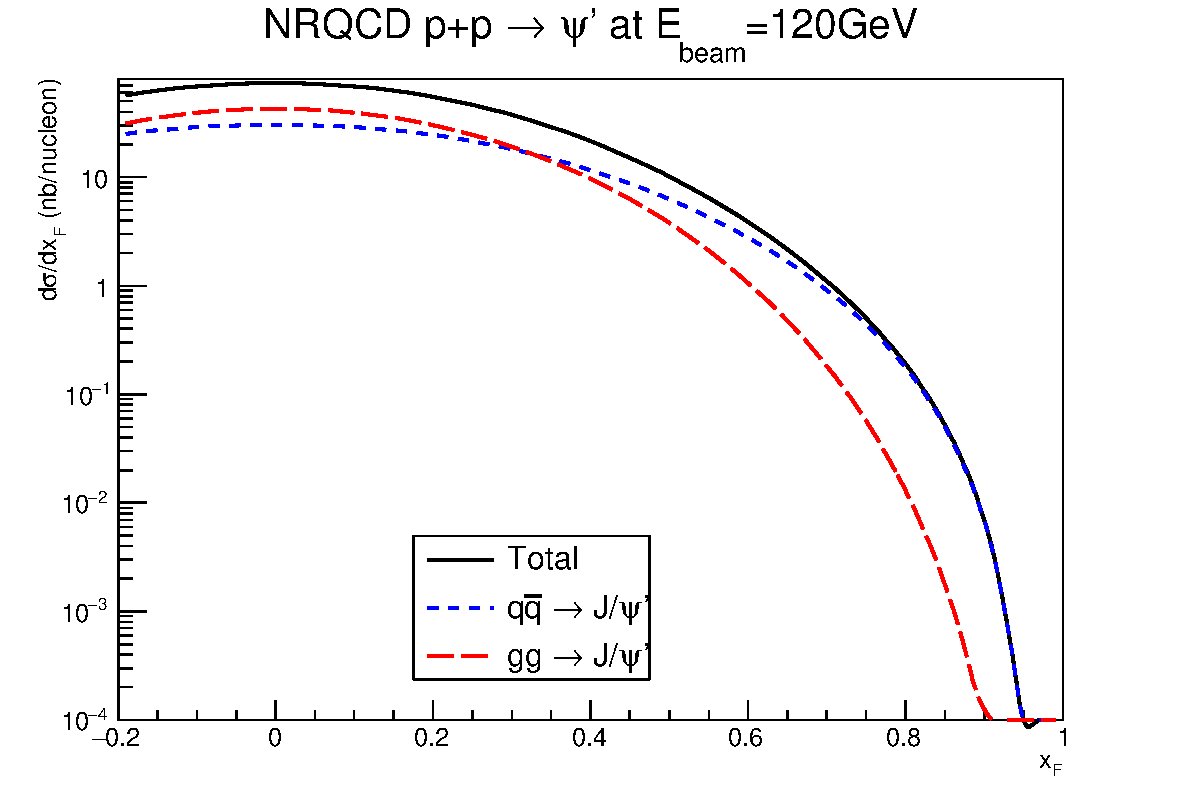
\includegraphics[width=\linewidth]{jpsi_cs_pp}
		\caption{$J/\psi$ production.}
	\end{subfigure}
	\quad
	\begin{subfigure}{0.45\linewidth}
		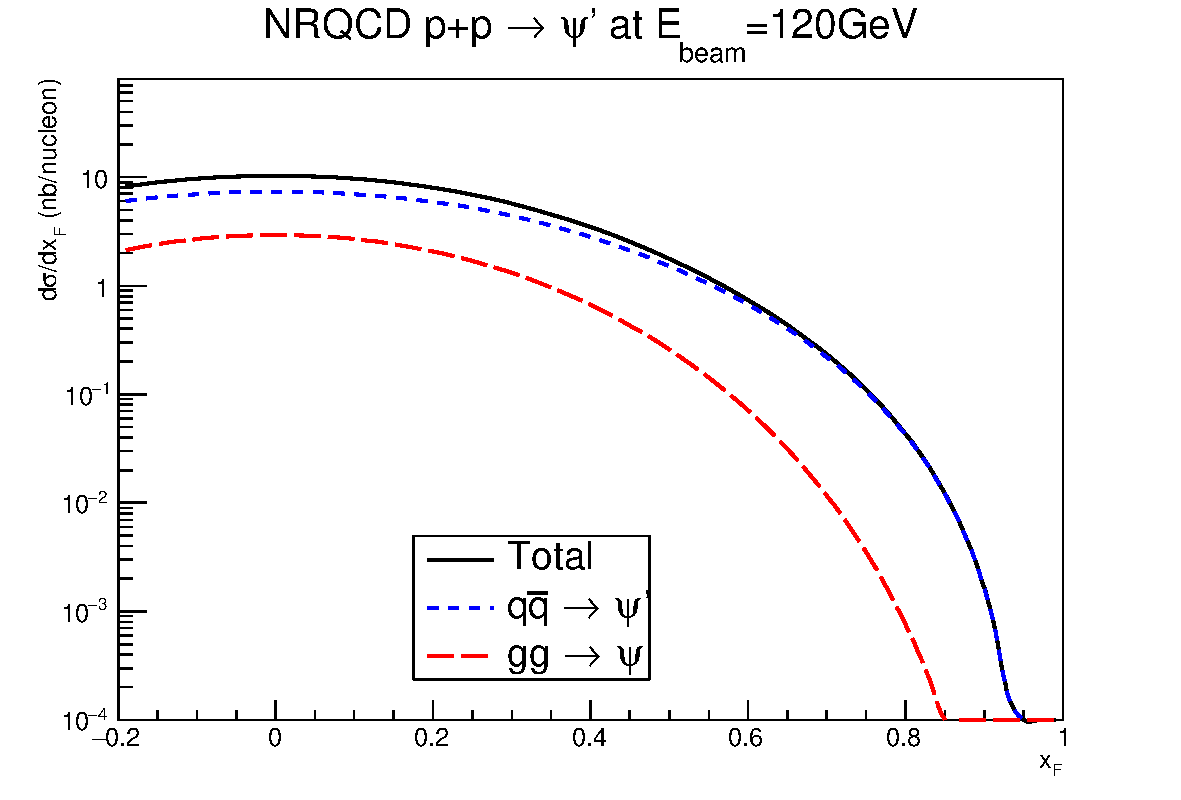
\includegraphics[width=\linewidth]{psip_cs_pp}
		\caption{$\psi'$ production.}
	\end{subfigure}
	\caption{Calculated cross section for charmonium production using NRQCD model
		\cite{chang2023a}. CT14nlo is used as the proton PDF. The LDMEs used are
		taken from Table \num{3} in Ref.~\cite{chang2023}, and are obtained from a
		global fit to fixed-target charmonium production data. }
	\label{fig:NRQCD_cs}
\end{figure}



\ifSubfilesClassLoaded{ \printbibliography[heading=bibintoc,title={References}]}{}

\end{document}


\chapter{SeaQuest Experiment}
\label{ch:seaquest}
\documentclass[../main.tex]{subfiles}
\begin{document}

\ifSubfilesClassLoaded{
	\mainmatter
	\setcounter{chapter}{3}
}{}

\chapter{SeaQuest Experiment}
\label{ch:seaquest}

\section{Introduction}
Following the E866 results~\cite{towell2001}, there were great interest in improving
the determination of the light sea-quark asymmetry at large $x$ and to understand
the drop in $\bar{d}/\bar{u}$ at $x>0.25$.
The E906 SeaQuest experiment was proposed as a follow-up to the E866 measurement \cite{isenhower2001}.
The main objective of the experiment is to probe the light sea-quark asymmetry at
large $x$ with better accuracy than previous measurement through the use of the Drell-Yan
process. To gain better statistics at large $x$, the \SI{120}{\GeV} proton beam from the Main
Injector is used instead of the \SI{800}{\GeV} beam from the Tevatron used during E866.
Since the Drell-Yan cross section is inversely proportional to the center-mass energy
squared, the lower beam energy allows for better statistics as large values of $x$.

\section{Beam}
The layout of the Fermilab accelerator complex is shown in \cref{fig:complex},
taken from Ref.~\cite{concept-book}.
SeaQuest received its \SI{120}{\GeV} proton beam from the Fermilab Main Injector.
The proton beam originate from a direct-extraction magnetron hydrogen ion source,
which produces a \SI{35}{\keV} negative hydrogen ion beam. It is then accelerated
to \SI{750}{\keV} using Radio-Frequency Quadrupole. Then the Linac accelerates the
$H^-$ ions to \SI{400}{\MeV}. The $H^-$ ions are then sent through a stripping foil
to remove the electrons. The resulting proton beam then circulates in the Booster
accelerator and accelerates to \SI{8}{\GeV}. The \SI{8}{\GeV} proton beam is
further accelerated by the Main Injector to \SI{120}{\GeV}. The proton beam is
extracted from the Main Injector using a process known as resonant extraction to
provide a lower intensity beam over a 5-second spill, with one spill per minute. The extracted beam, which
is sent to SeaQuest, retains the \SI{53.1}{\MHz} structure of the Main
Injector RF frequency, dividing the beam into ``RF buckets'' that are less than
\SI{2}{\ns} long and occur every \SI{18.8}{\ns}.
\begin{figure}[htbp!]
	\centering
	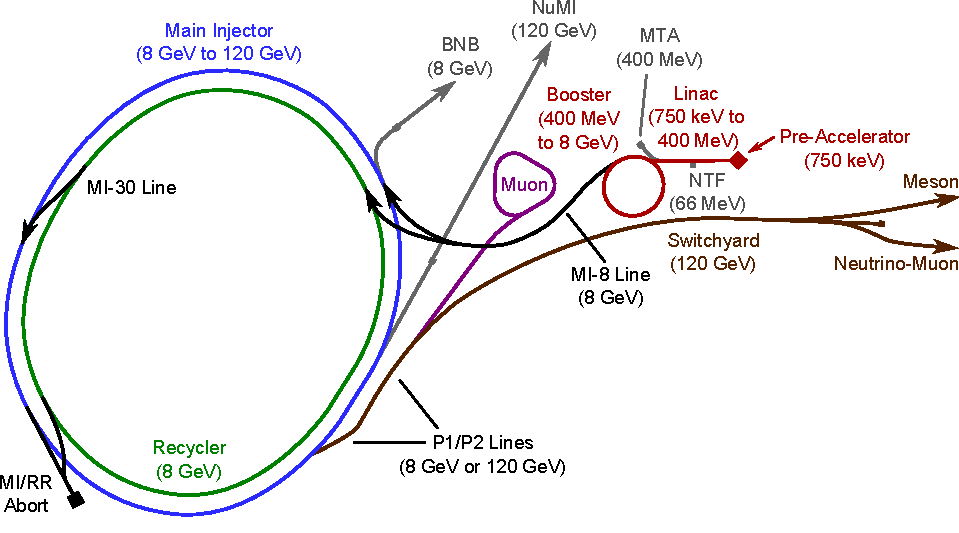
\includegraphics[width=0.6\linewidth]{Fermilab-complex}
	\caption{Layout of the Fermilab accelerator complex, taken from Ref.~\cite{concept-book}. The
		SeaQuest Experimental hall is located on the Neutrino-Muon beamline.}
	\label{fig:complex}
\end{figure}
Even though the integrated intensity from each spill is very stable,
the number of protons in each bucket can vary greatly during the spill, as
is shown in \cref{fig:intensity}.
\begin{figure}[htpb!]
	\centering
	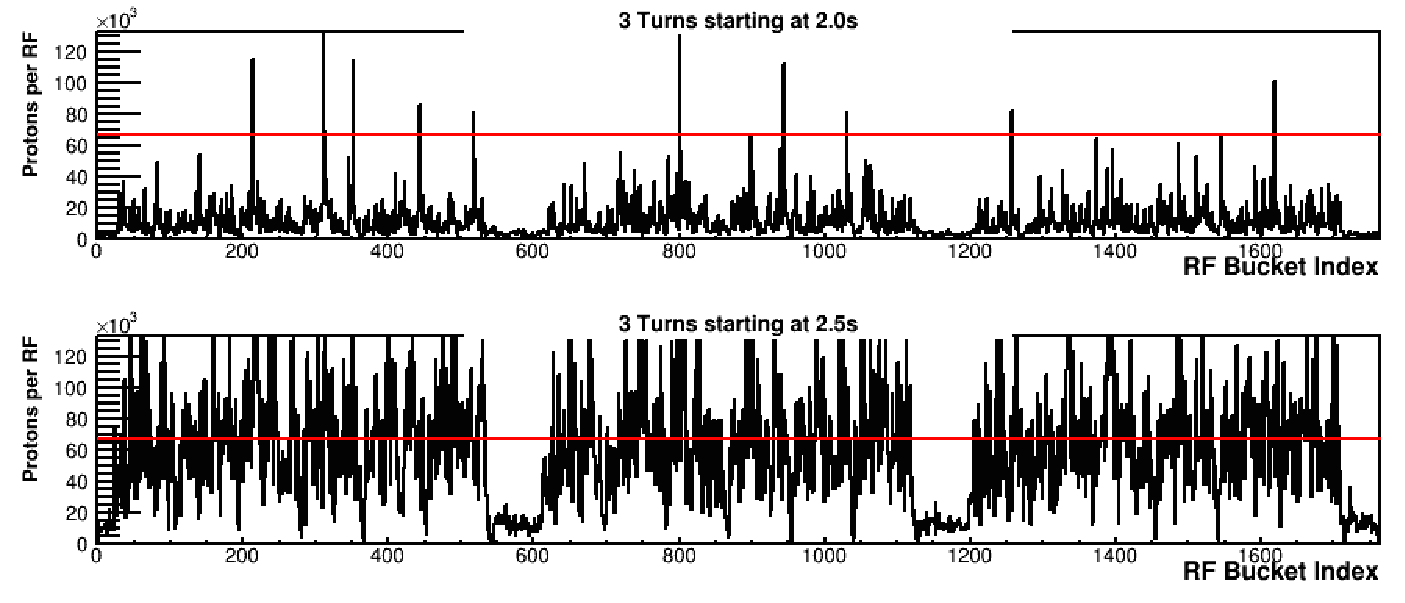
\includegraphics[width =0.8\linewidth]{beam_intensity_v2}
	\caption{The beam intensity measured by the Beam DAQ Cerenkov counter every
		bucket. Taken from Ref.~\cite{aidala2019}}
	\label{fig:intensity}
\end{figure}

\subsection{Beam Intensity Monitor}
\label{subsec:BIM}
The integrated beam intensity is monitor by Fermilab Accelerator Division using a
secondary emission monitor located upstream of the SeaQuest experimental hall.
To better understand the bucket-to-bucket variation in the beam intensity, a Cerenkov counter,
shown in \cref{fig:BIM}, was added upstream of the target during the Main Injector upgrade.
\begin{figure}[htbp!]
	\centering
	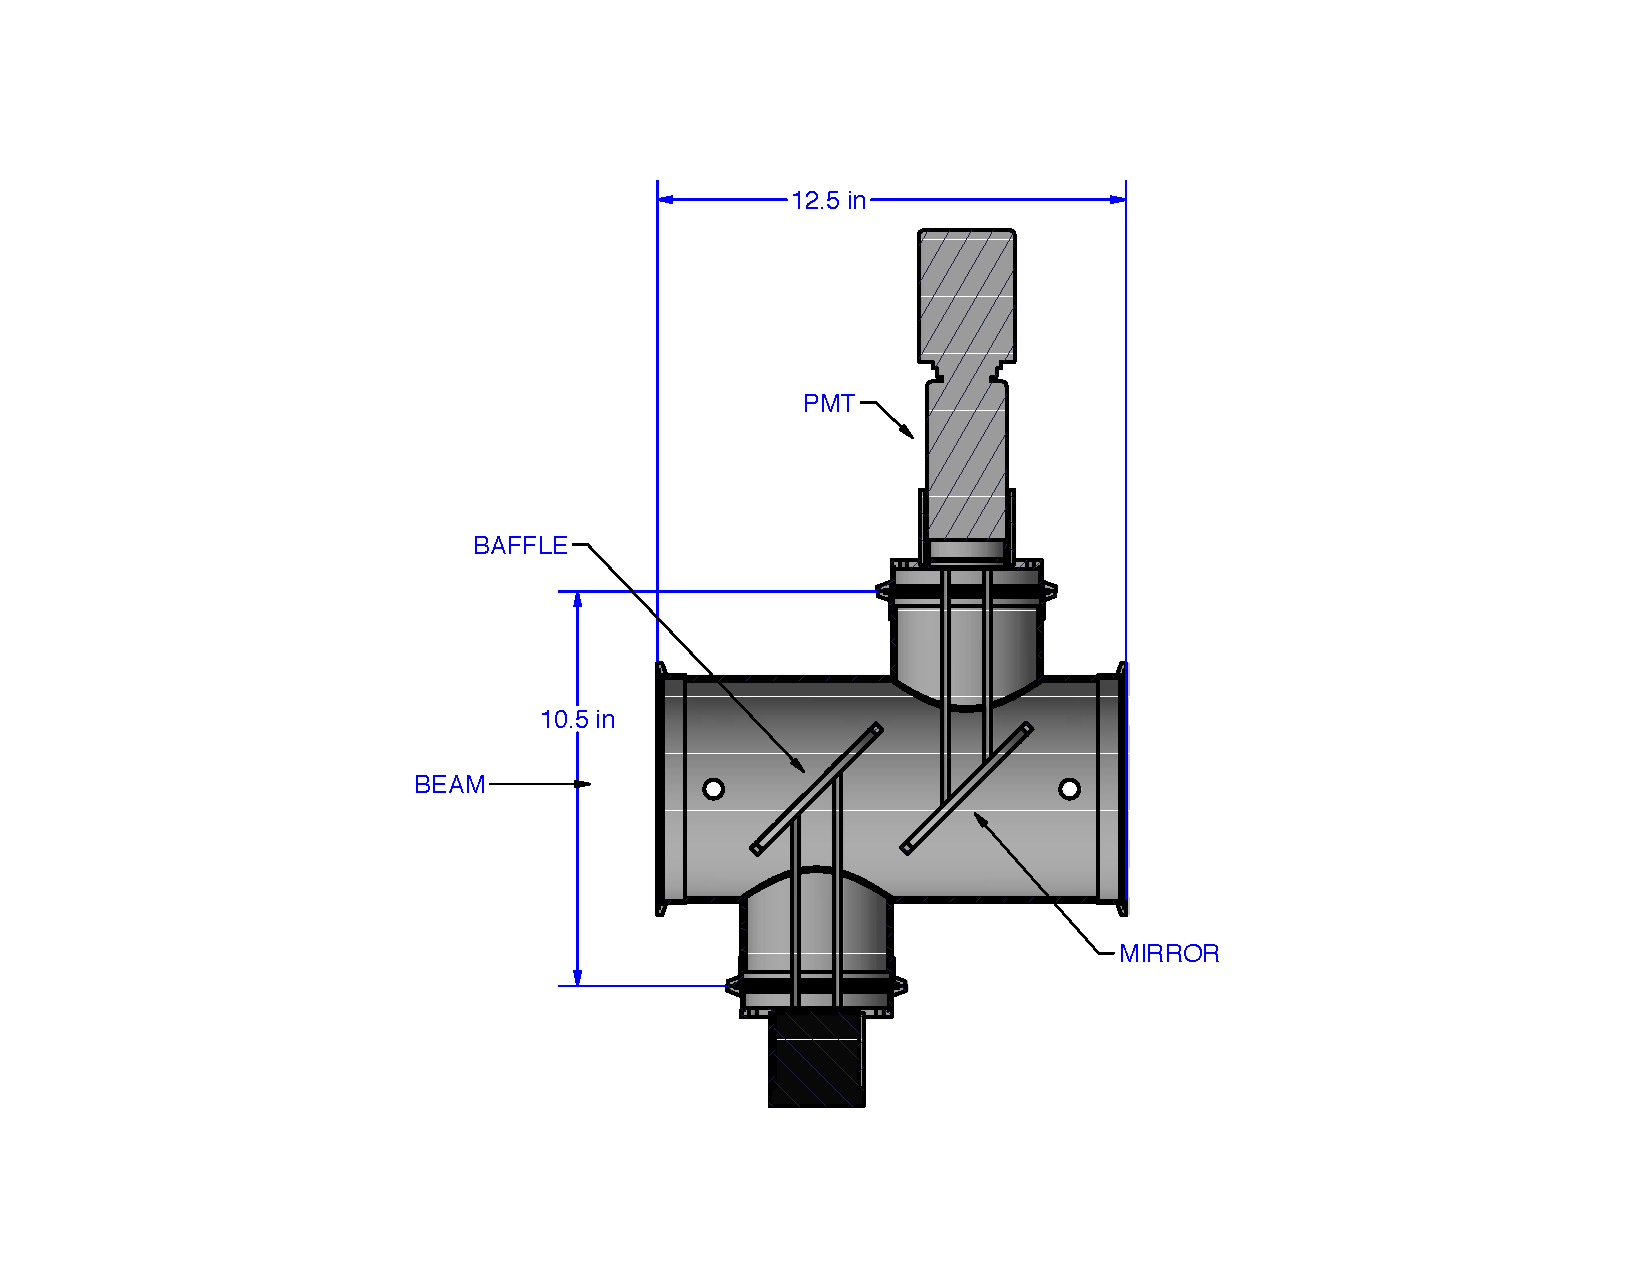
\includegraphics[width=0.4\linewidth]{BIMCerenkov}
	\caption{The Beam Intensity Monitor (BIM) Cerenkov counter. Taken from Ref.\
		\cite{aidala2019}.}
	\label{fig:BIM}
\end{figure}

An aluminized Kapton mirror reflects the Cerenkov light, produced when the proton beam
pass through the radiator, into a single photomultiplier tube. The signal is then
sent to a custom ``QIE'' (Charge Integrator and Encoder) module. This custom module
is clocked with the Main Injector RF, and is capable of recording the beam intensity
of each RF bucket for the entire spill. The QIE module is linked to the trigger
system, and would raise a trigger inhibit when the beam intensity is above a
threshold. The module is also read out by the Beam DAQ, which will be discussed
in \cref{subsec:beamDAQ}. 
The beam intensity monitor is calibrated against a secondary emission monitor.

The ability to record the numbers of proton in each bucket allows us to obtain the
yields as a function of the instantaneous intensity, which will be discussed
further in \cref{M-sec:extrapolation}.

\section{Target}
The SeaQuest target is placed between the Beam Intensity Monitor and the front face
of spectrometer. The target system consists of two liquid targets, hydrogen and deuterium,
and three solid targets, iron, carbon and tungsten. Each solid target is divided
into \num{3} discs of equal length, and are spatially separated along the beam
direction to minimize variation in acceptance between liquid and solid targets.
To account for background originating from the interaction with the instruments,
there are also two calibration targets, an empty vacuum filled flask, known as
empty flask, and the solid target holder, known as no-target. The different targets
are mounted on a motorized table, shown in \cref{fig:target}, which allows the
targets to be interchanged between spills to minimized systematic effect due to
changes in spectrometer performance over time. The properties of the targets and the spills per cycle
of each target positions are listed in \cref{table:target}.
\begin{figure}[htbp!]
	\centering
	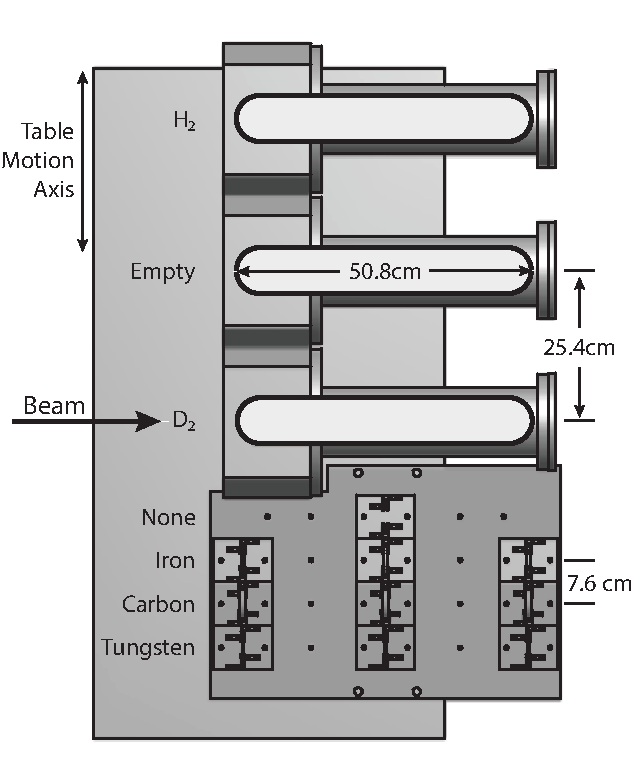
\includegraphics[width=0.4\linewidth]{target-tableLayout}
	\caption{The schematic of the movable target table}
	\label{fig:target}
\end{figure}

\begin{table}[h!]
	\centering
	\caption{SeaQuest target configuration}
	\label{table:target}
	\begin{tabular}{cccccc}
		\hline
		Target      & Position & Density (\unit{\g\per\cm\cubed}) & length (\unit{\cm}) & interaction length   (\unit{\g\per\cm\squared}) & spill/cycle \\ \hline
		\ce{LH_2}   & 1        & \num{0.071}                      & \num{50.8}          & \num{52.0}                                      & 10          \\
		Empty Flask & 2        & -                                & -                   & -                                               & 2           \\
		\ce{LD_2}   & 3        & \num{0.1634}                     & \num{50.8}          & \num{71.8}                                      & 5           \\
		No target   & 4        & -                                & -                   & -                                               & 2           \\
		Iron        & 5        & \num{7.87}                       & \num{1.905}         & \num{132.1}                                     & 1           \\
		Carbon      & 6        & \num{1.80}                       & \num{3.322}         & \num{85.8}                                      & 2           \\
		Tungsten    & 7        & \num{19.30}                      & \num{0.953}         & \num{191.9}                                     & 1           \\
		\hline
	\end{tabular}
\end{table}

\section{Spectrometer and Tracking Station}
The SeaQuest spectrometer consists of two magnets and four tracking stations. A solid iron magnet,
FMag, is placed \SI{104}{\cm} downstream the target. It is then followed by
the first tracking stations. The SeaQuest detector system is separated into four tracking stations.
Stations 1, 2 and 3 each consists of plastic scintillator hodoscopes and drift chambers.
The hodoscopes in each stations provides a fast signal for triggering whereas
the drift chambers provide good spatial resolution for track precise reconstruction.
An open air dipole magnet (KMag) is placed between station 1 and station 2.
Downstream of station 3, there is a 1 m iron wall acting as a
hadron absorber. Station 4 is located behind the hadron absorber and acts as a
muon identifier. Station 4 consists of a hodoscope array and 4 layers of
proportional tube planes.

\begin{figure}[htbp!]
	\centering
	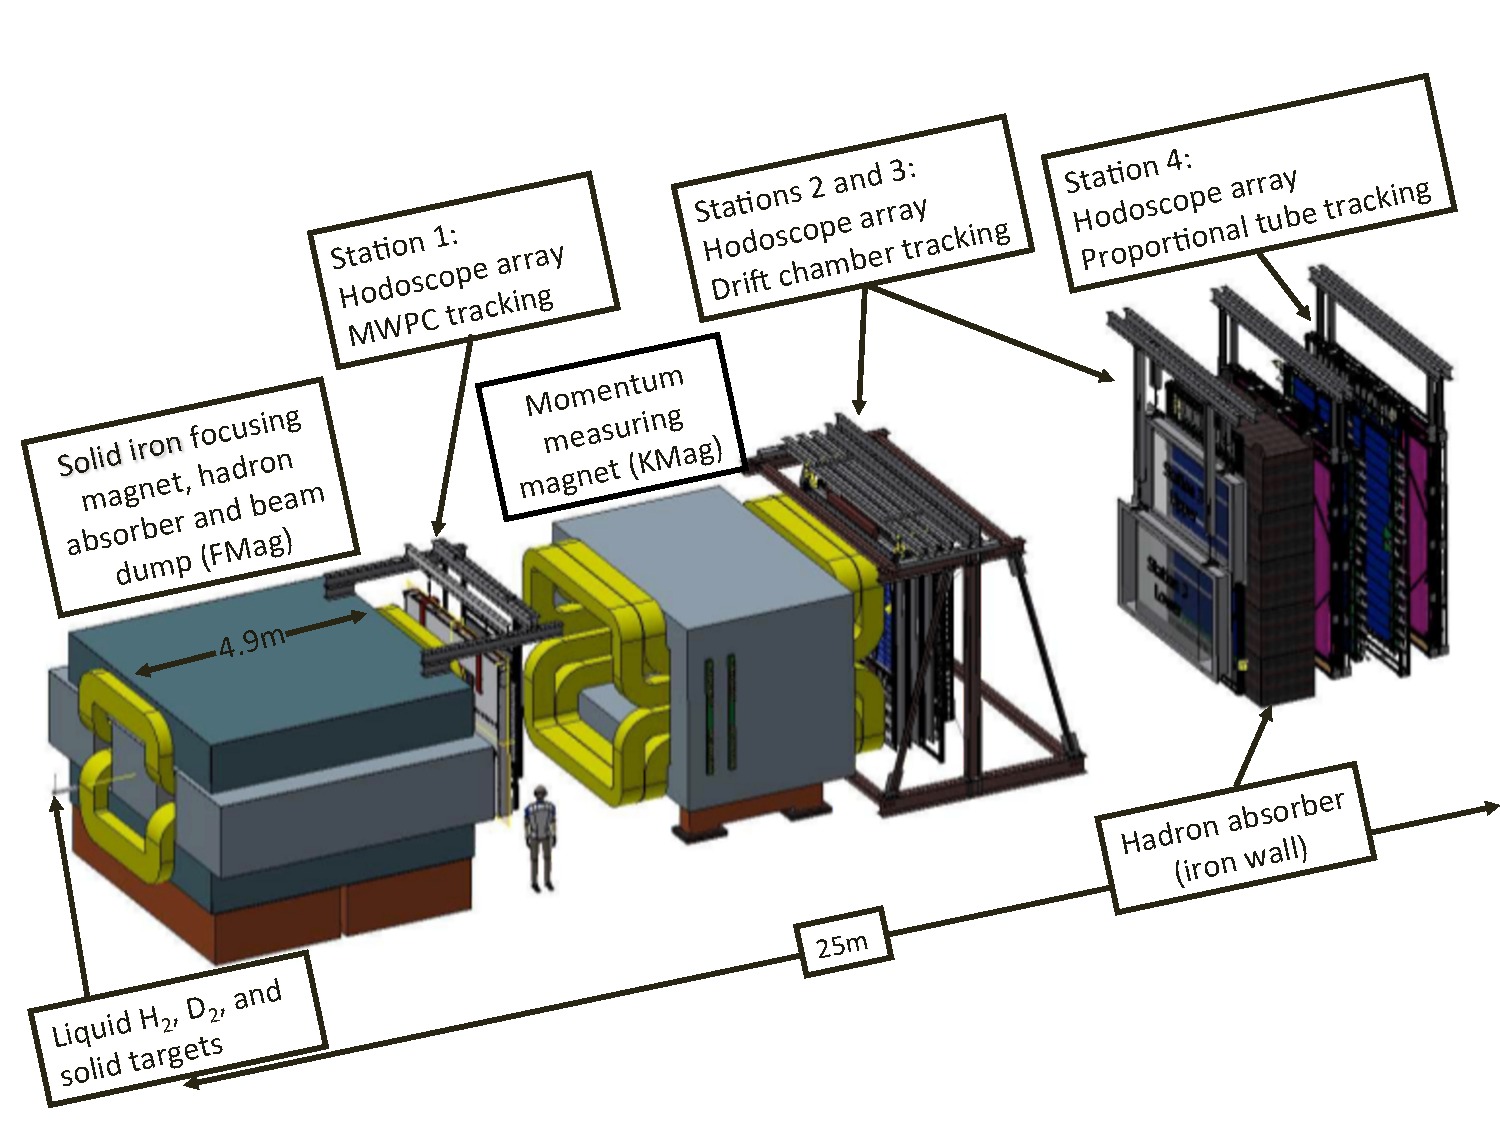
\includegraphics[width=0.6\linewidth]{SeaQuestSpectrometer}
	\caption{schematics of the SeaQuest spectrometer. Taken from Ref.~\cite{aidala2019}}
	\label{fig:spectrometer}
\end{figure}

\subsection{Magnets}
There are two dipole magnets used in the SeaQuest spectrometer, namely the focusing
magnet (FMag) and analyzing magnet (KMag). The magnetic field of both magnets point
in the same direction vertically ($\pm y$), which bend the muons horizontally along
the $x-z$ plane. The polarity of the magnets were flipped during Run 3, partly to reduce
radiation damage to electronics located in the hall.

The upstream focusing magnet (FMag) is a solid iron magnet, shown in \cref{fig:fmag}.
It measures at \SI{503}{\cm} by \SI{302.4}{\cm} tall by \SI{160}{\cm} wide.
The magnet consists of a stack of high purity iron, recovered from
the Columbia University Nevis Laboratory Cyclotron, and the aluminium coils from the E866
SM3 magnet. The coils are excited to \SI{2000}{\ampere} and generate an \SI{1.9}{\tesla}
magnetic field within the iron block. This corresponds to a transverse momentum kick of
\SI{3.07}{\GeV}. FMag serves three main purposes: focusing high mass muon pairs, beam
dump and hadron absorber. As a focusing magnet, FMag would focus dimuons with high $p_T$
or high mass into the spectrometer acceptance. This is particularly important as SeaQuest
aims to probe the partonic structure at high $x$, which would correspond to high mass.
Additionally, it would also defocus the low momentum muons, hence reducing the background.
Due to the high beam intensity, FMag also serves as beam dump. Typically, only $\sim 10\%$
of the proton beam would interact with target material. The remaining protons would interact
within FMag. The hadrons produced during this process would also be absorbed by the iron,
while allowing muons into the spectrometer.
A \SI{5}{\cm} diameter by \SI{25}{\cm} deep hole is drilled into the upstream
end of FMag along the beam axis. This is done to move the initial interaction points
of the beam with the beam dump further away from the targets, allowing for better target/dump
separation. This also reduces the radiation within the target cave, which facilitate the
access to the target area for maintenance.
The magnetic field distribution is modeled using a magnetostatic modeling program. The
excitation is measured by wrapping a 1-turn coil around the central region of the magnet to measure the induced
current. Final calibration of the field strength is determined by the reconstructed
mass of the $J/\psi$ resonance.
\begin{figure}[h!]
	\centering
	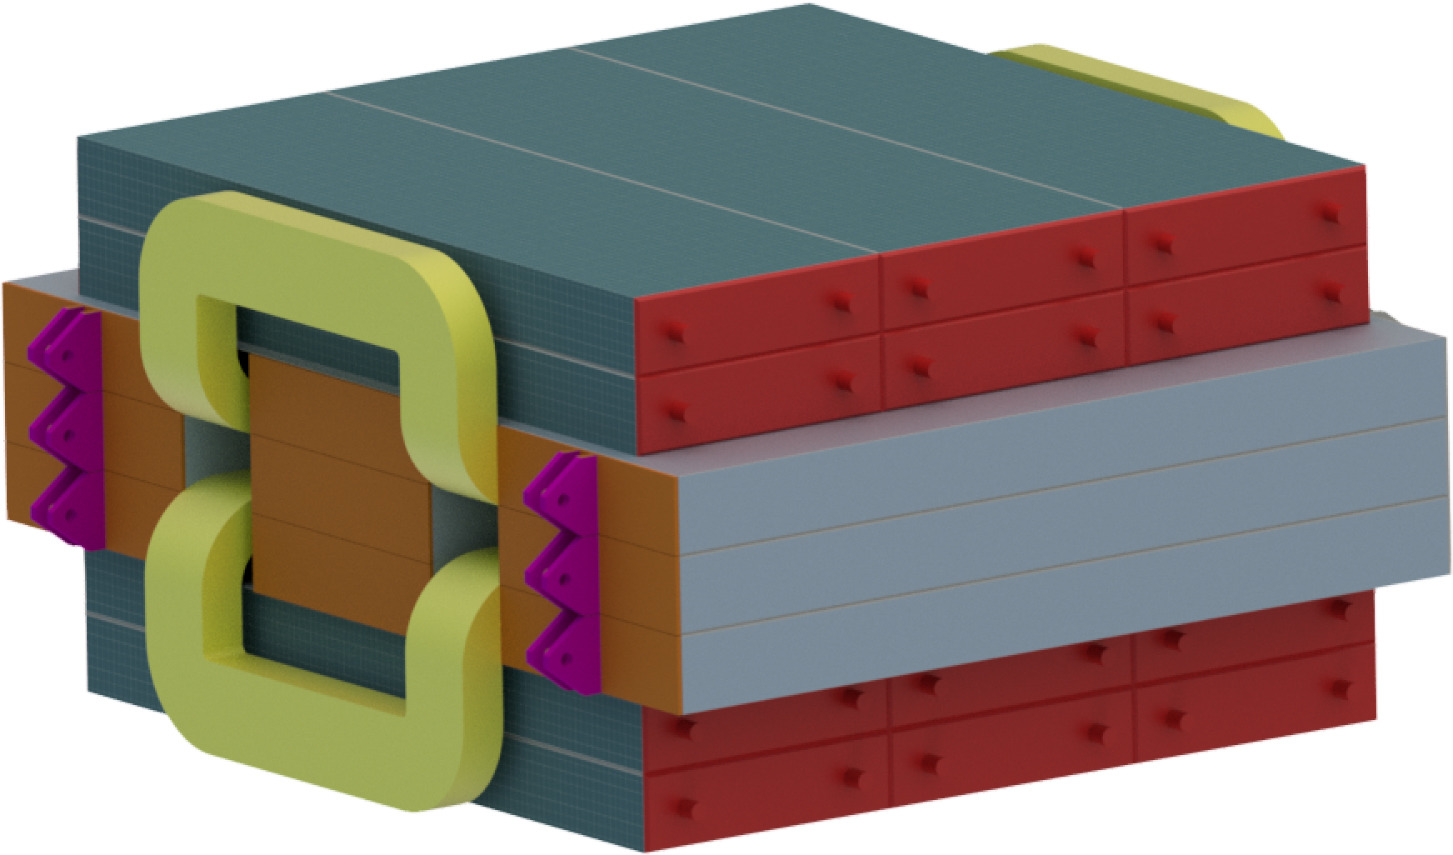
\includegraphics[width=0.5\linewidth]{FMAG}
	\caption{Perspective drawing of FMag showing the arrangement of the iron slabs.
		Taken from Ref.~\cite{aidala2019}.}
	\label{fig:fmag}
\end{figure}

The downstream analyzing magent (KMag) is a \SI{3}{\meter} long open aperture magnet
with a \SI{289}{\cm} wide by \SI{203}{\cm} high central air gap. It was
originally  constructed by E799/KTeV collaboration\cite{alavi-harati2003}.
The coils are excited to \SI{1600}{\ampere} which produce a magnetic field of \SI{0.4}{\tesla},
corresponding to a \SI{0.41}{\GeV} transverse momentum kick. The primary purpose for
KMag is to determine the momentum of the muons. The magnetic field is measured using a Hall
probe and is further calibrated using the reconstructed mass of the $J/\psi$ resonance.


\subsection{Hodoscope}
A hodoscope is placed on upstream end of each tracking stations. Each of the hodoscope planes
is composed of overlapping panels of scintillators viewed by photomultiplier tubes (PMTs) at the end.
When a charged particle pass through the scintillator, the molecules would be excited and
release photons. These photons are then collected at the PMTs, the amplified signals are
then send through discriminators. The signal is then recorded by the Data Acquisition (DAQ) System
using Time-to-Digital converters (TDCs).
The primary purpose of the scintillator hodoscopes is to provide fast signal for the
trigger system. It is also used during reconstruction to reduce the number of chamber hits.
The x-planes are placed vertically to measure the bend plane position.
And the y-planes are arranged horizontally to measure the non-bend plane position.
The scintillator bars in each plane is also split in the middle, denoted as Top and Bottom
for the x-planes, or Left and Right for the y-planes.

Station~1 and 2 each have single x-y planes. Station~3 has a single x plane, and station
4 has two y planes and one x plane. The scintillator bars used in St~.1 and 2 are recycled
from HERMES experiment~\cite{ackerstaff1998a}, whereas new Eljen EJ-200 scintillator material
is used for St.~3 and 4. Because of the physical size of the sintillatior bars in St.~4, the station~4
hodoscopes have PMTs on both ends of the sintillator bars. Each of the PMT base has a
``clip line'' attached at the output to reduce the output pulse from $20-25$\unit{\ns}
down to $10-15$\unit{\ns} full width.

The configuration of the hodoscope is summarized in \cref{table:hodo}. \pdfmargincomment{why are there 2 y hodo in St4? Lower rate at St4? Shivangi's thesis is correct NIM paper is wrong}
\begin{table}[h!]
	\centering
	\caption{SeaQuest hodoscope configuration}
	\label{table:hodo}
	\begin{tabular}{lllllll}
		\hline
		Plane & Number      & Length (\unit{\cm}) & Width (\unit{\cm}) & Thickness (\unit{\cm}) & Array Width (\unit{\cm}) & Location (\unit{\cm})                                                 \\ \hline
		1Y    & $20\times2$ & \num{78.7}          & \num{7.32}         & \num{0.64}             & \num{140}                & \num{667}                                                             \\
		1X    & $23\times2$ & \num{69.9}          & \num{7.32}         & \num{0.64}             & \num{161}                & \num{654}                                                             \\
		2Y    & $19\times2$ & \num{132.0}         & \num{13.0}         & \num{0.64}             & \num{241}                & \num{1402}                                                            \\
		2X    & $16\times2$ & \num{152.0}         & \num{13.0}         & \num{0.64}             & \num{203}                & \num{1421}                                                            \\
		3X    & $16\times2$ & \num{167.6}         & \num{14.6}         & \num{1.3}              & \num{224}                & \num{1958}                                                            \\
		4Y1   & $16\times2$ & \num{152.4}         & \num{23.5}         & \num{1.3}              & \num{366}                & \begin{tabular}[c]{@{}l@{}}\num{2130}(L)\\ \num{2146}(R)\end{tabular} \\
		4Y2   & $16\times2$ & \num{152.4}         & \num{23.5}         & \num{1.3}              & \num{366}                & \begin{tabular}[c]{@{}l@{}}\num{2200}(L)\\ \num{2217}(R)\end{tabular} \\
		4X    & $16\times2$ & \num{182.9}         & \num{19.6}         & \num{1.3}              & \num{305}                & \begin{tabular}[c]{@{}l@{}}\num{2236}(T)\\ \num{2251}(B)\end{tabular} \\
		\hline
	\end{tabular}
\end{table}

\subsection{Drift Chambers}
The resolution of the hodoscope is limited by the physical size of the scintillator bars.
Drift chamber are used to provide a better position resolution of the muons at each station.
A drift chamber measures the position by recording the drift time of the electrons created
by the ionization of the gas mixture when charged particles pass through the chamber.
Each drift chamber consist of six planes of sense wires. The wires in two planes,
denoted as X and X$'$, are aligned vertically. Two planes are tilted by \ang[retain-explicit-plus]{+14},
denoted as U and U$'$, and two planes, V and V$'$, are tilted by \ang[retain-explicit-plus]{-14}.
The wires in the primed planes are offset by half a drift cell relative to the
unprimed planes to resolve left-right ambiguity of the drift direction.
Station 1 and 2 each have one chamber referred as D1 and D2. The chamber at station
3 is separated into top and bottom halves, denoted as D3p and D3m.

In data sets 1-3, a smaller chamber, D1.1, was used. It was later replaced by a newly constructed
chamber, D1.2, with better expected high rate capacity in data set 4-6. However, D1.1 would be
reinstalled later for data set 5-6. D3m.1 was used during the commissioning run, data set 1, and
was later replaced by D3m.2 for the later data sets.

The D1.1, D2 and D3m.1 chambers were recycled from previous Fermilab experiments, E605 (D2 and D3m.1)~\cite{moreno1991}
and E866 (D1.1)~\cite{hawker1998}. The other chambers were designed and constructed for the SeaQuest experiment.
Specifications of each chamber are listed in \cref{table:chamber}.

The signals from the sense wires are fed to ASDQ (Amplification, Shaper, Discriminator and Charger integrator)
cards which are used for amplification and discrimination. The signal is then fed to LSB (Level Shifter Board)
to covert into standard LVDS (low voltage differential signal), which can then be read out by the TDC
modules and recorded by the DAQ system.

\begin{table}[h!]
	\centering
	\caption{SeaQuest drift chamber configuration. The primed planes are almost the same as the unprimed
		planes. The positions of the X planes are defined to be the distance between the chamber and the
		upstream face of FMag, while the positions for U and V denote the offset relative to the corresponding
		X plane.}
	\label{table:chamber}
	\begin{tabular}{cccccc}
		\hline
		Chamber & Plane & \# of wires & Cell width (\unit{\cm}) & Width\texttimes Height (\unit{\cm}\texttimes\unit{\cm}) & z Position (\unit{cm}) \\ \hline
		D1.1    & X     & \num{160}   & \num{0.64}              & $102\times 122$                                         & \num{617}              \\
		        & U, V  & \num{201}   & \num{0.64}              & $101\times 122$                                         & $\pm20$                \\
		D1.2    & X     & \num{320}   & \num{0.50}              & $153\times 137$                                         & \num{691}              \\
		        & U, V  & \num{384}   & \num{0.50}              & $153\times 137$                                         & $\pm1.2$               \\
		D2      & X     & \num{112}   & \num{2.1}               & $233\times264$                                          & \num{1347}             \\
		        & U, V  & \num{128}   & \num{2.0}               & $233\times264$                                          & $\pm25$                \\
		D3p     & X     & \num{116}   & \num{2.0}               & $232\times166$                                          & \num{1931}             \\
		        & U, V  & \num{134}   & \num{2.0}               & $268\times166$                                          & $\pm6$                 \\
		D3m.1   & X     & \num{176}   & \num{1.0}               & $179\times168$                                          & \num{1879}             \\
		        & U, V  & \num{208}   & \num{1.0}               & $171\times163$                                          & $\pm19$                \\
		D3m.2   & X     & \num{116}   & \num{2.0}               & $232\times166$                                          & \num{1895}             \\
		        & U, V  & \num{134}   & \num{2.0}               & $268\times166$                                          & $\pm6$                 \\ \hline
	\end{tabular}
\end{table}

\subsection{Proportional tubes}
The muon identification is accomplished with the proportional tube at station 4. A \SI{1}{\meter} thick
iron wall separate station 3 and 4, which acts as an absorber to stop hadrons and electrons from reaching
station 4. For precise track reconstruction, there are four layers of proportional tubes planes. Each plane
is made of eight proportional tube modules, with 16 proportional tubes per module. The 16 proportional tubes
in each module further divided into two sub-layers, with the second layers shifted by half a tube width to
resolve the left-right ambiguity, as in the case of drift chambers. The proportional tubes oriented horizontally
(vertically) are in the first and fourth (second and third) planes as shown in \cref{fig:prop}
\begin{figure}[ht!]
	\centering
	\begin{subfigure}{0.45\linewidth}
		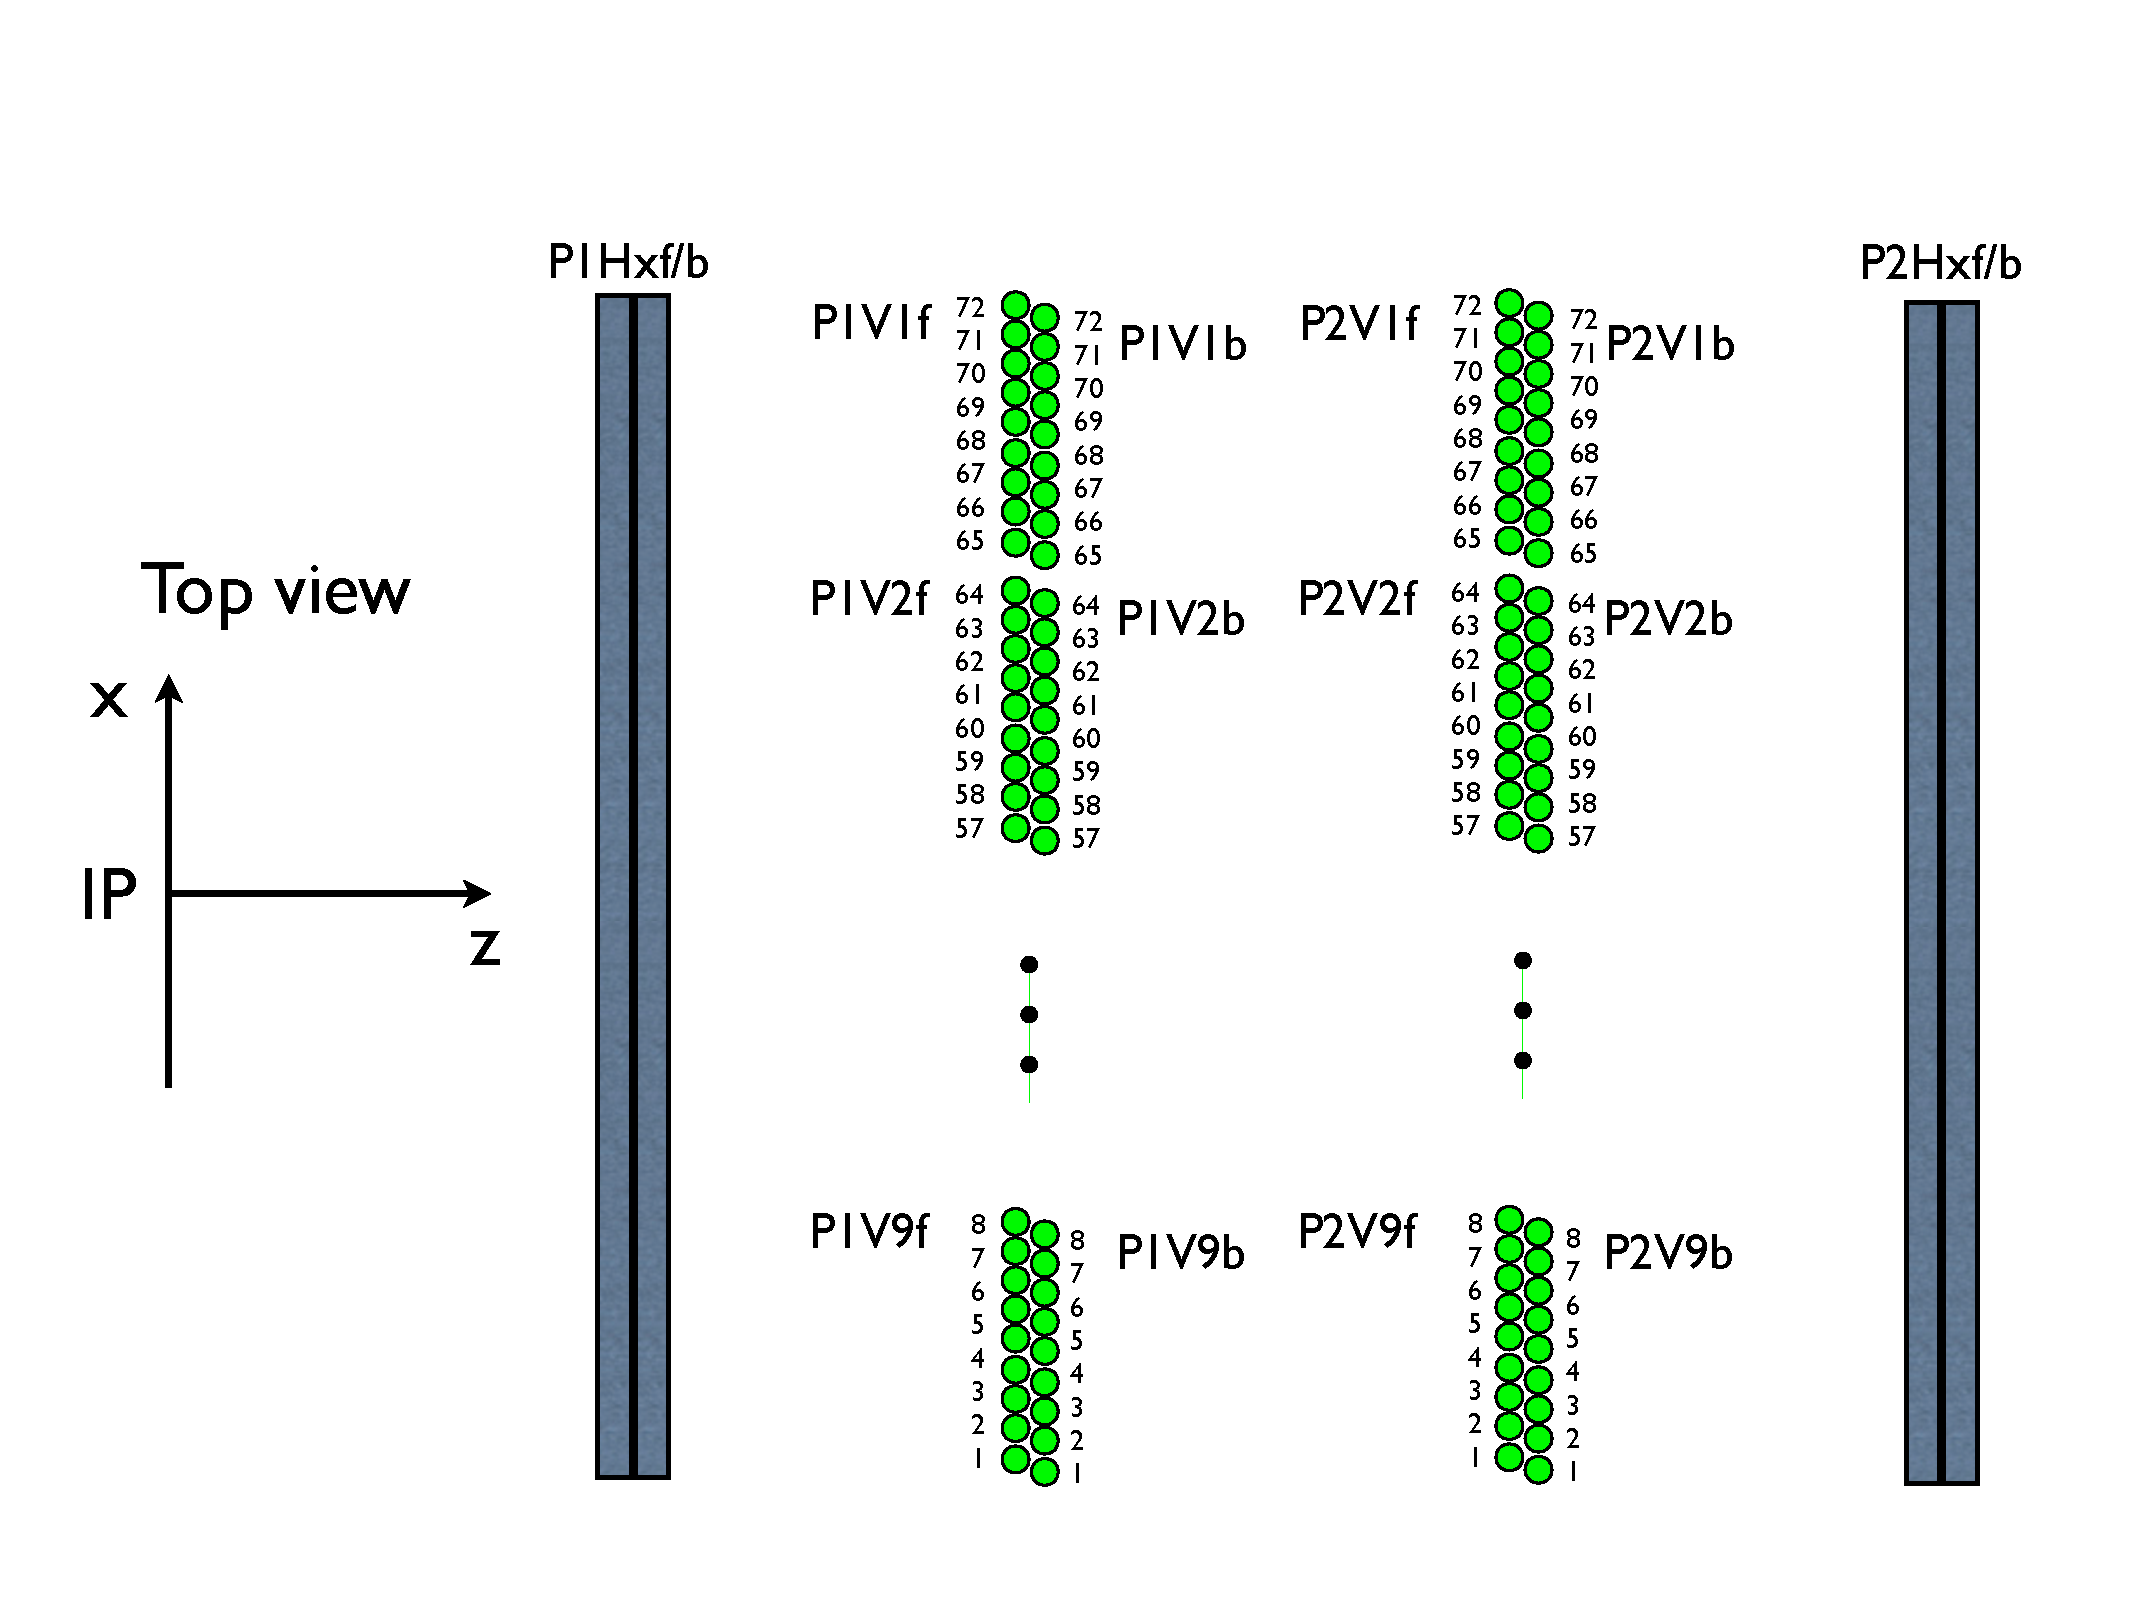
\includegraphics[width=0.9\linewidth]{proptubeview_xz}
	\end{subfigure}
	\begin{subfigure}{0.45\linewidth}
		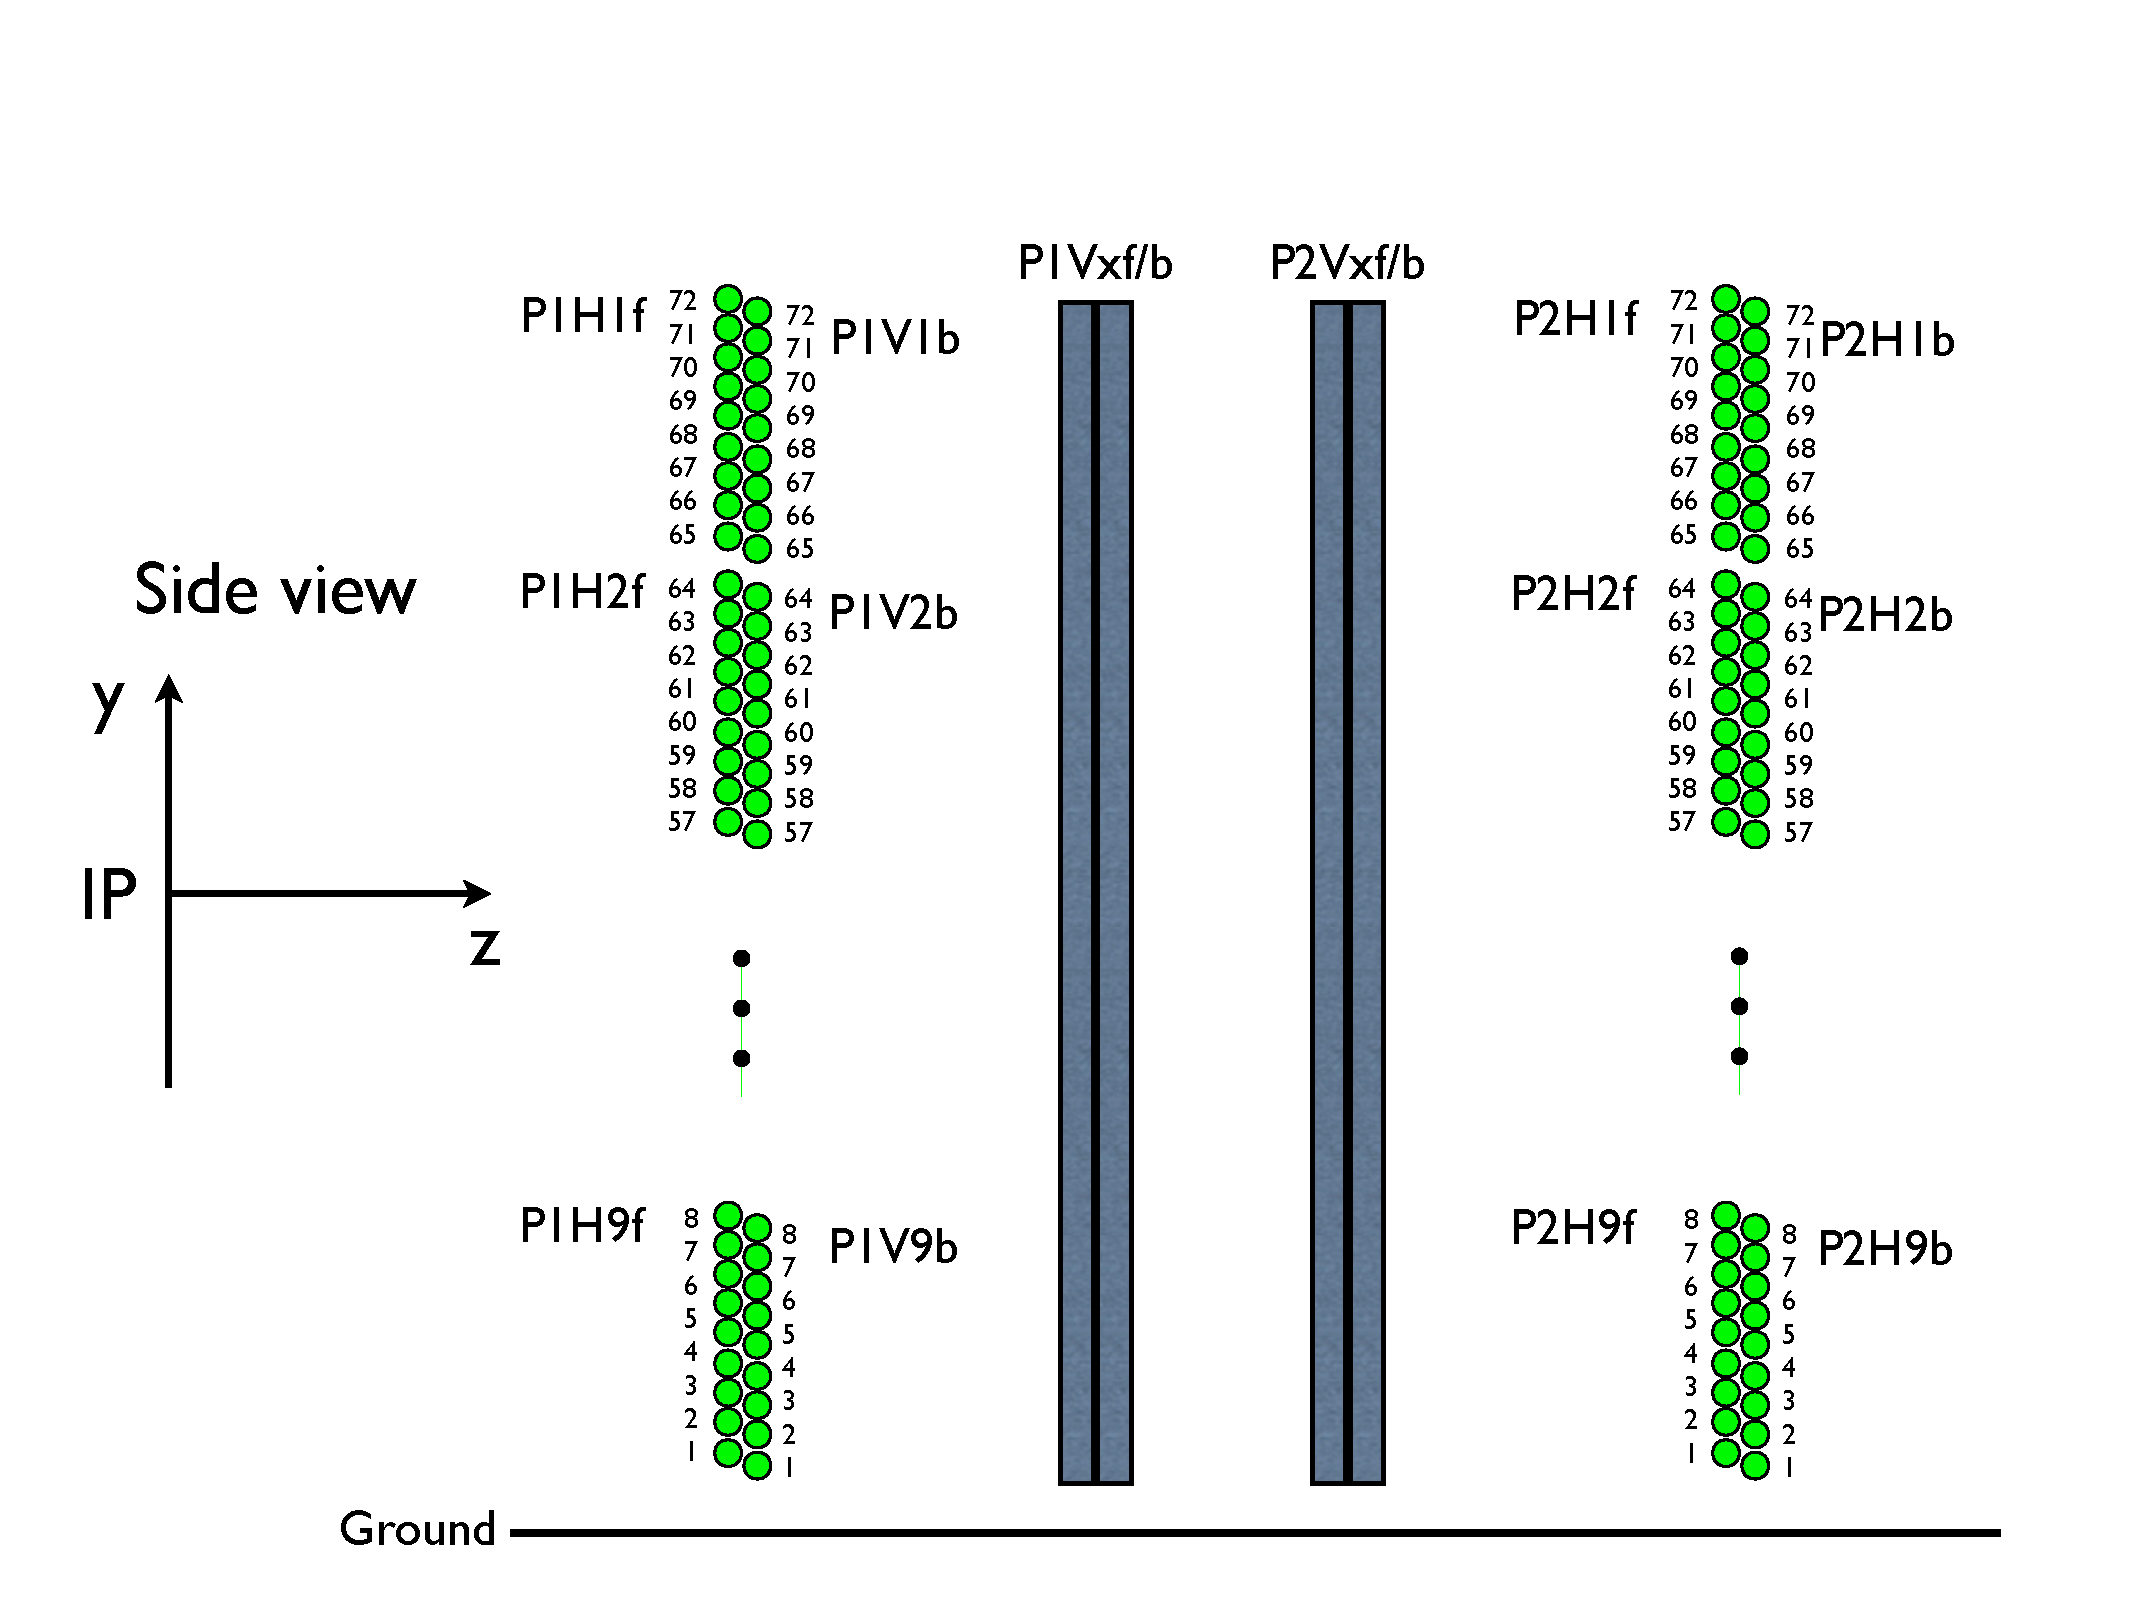
\includegraphics[width=0.9\linewidth]{proptubeview_yz}
	\end{subfigure}
	\caption{XZ (left) and YZ (left) view of the proportional tube at station 4.}
	\label{fig:prop}
\end{figure}
A typical high energy muons would traverse two proportional tubes in each planes.
For muon identification, 8 hits from 4 planes are required, and the hits
should also be pointing back at the target.

\section{Trigger System}
The SeaQuest trigger uses discriminated signals from the hodoscope counters.
Two separate trigger systems are used in SeaQuest, NIM-based and FPGA-based.
The FPGA trigger system is the main trigger system. It utilizes 9 CAEN
v1495 VME modules, Altera EP1C20F400C6 FPGA (Field Programmable Gate Array)
modules. The 9 modules are separated into three levels from level 0 to level
2, as illustrated in \cref{fig:trigger}.
Four FPGA modules form the level 0, with one module for each hodoscope
``quadrant'' (upper bend plane, lower bend plane, upper nonbend plane and
lower nonbend plane). During data taking, level 0 simply passes the input signal
to level 1. The level 0 can also act as a pulser for diagnostic purpose.
At level 1, four FPGA modules are used to search for four-hit track
candidates in each quadrant and compared with a preselected list of hit
patterns, known as trigger roads. The list of trigger roads (known as roadset)
are generated by studying the path of muons from Monte Carlo simulations, with
the goal of persevering signal rates while suppressing backgrounds.
The level 2 consists of a single module, and forms
a trigger decision based on types of track candidates found at level 1. During
SeaQuest data taking, there are five output triggers, as listed in \cref{tab:FPGA}.
During SeaQuest, only x-measuring (bend plane) hodoscopes are used in making
trigger decisions.
\begin{figure}
	\centering
	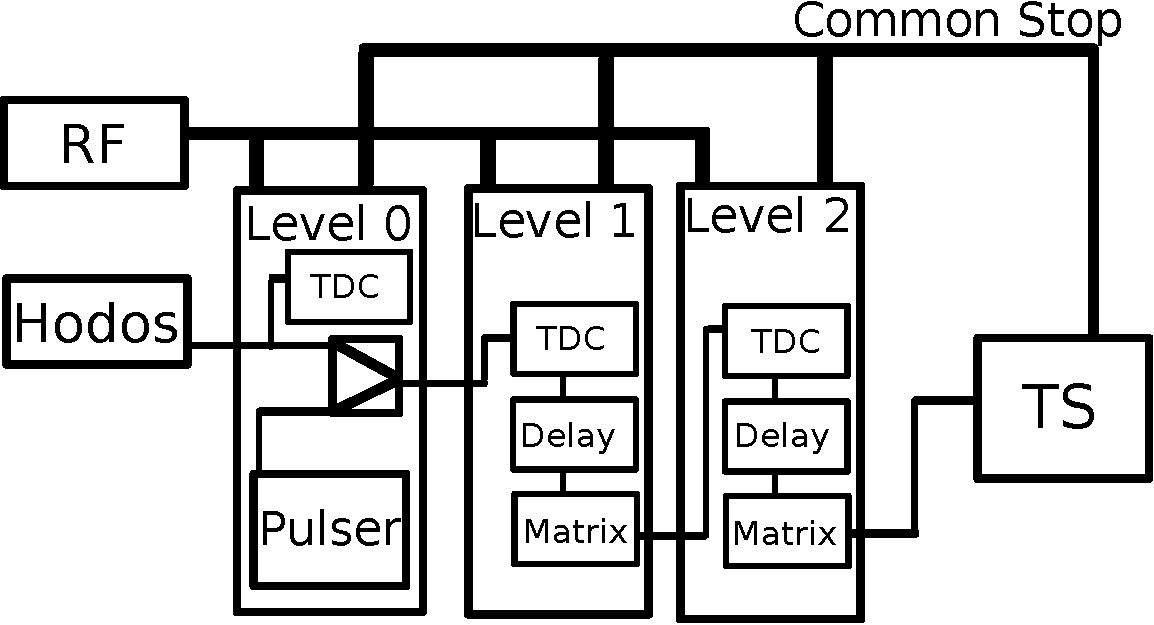
\includegraphics[width=0.5\linewidth]{trigger_schematic}
	\caption{The schematic of the FPGA trigger hardware}
	\label{fig:trigger}
\end{figure}
\begin{table}[h!]
	\centering
	\caption{The five output trigger of the Level 2 trigger module.}
	\label{tab:FPGA}
	\begin{tabular}{lllll}
		Name     & side  & Charge  & $p_x$ Req.         & Notes                     \\ \hline
		Matrix 1 & TB/BT & $+-/-+$ & None               & Main physics trigger      \\
		Matrix 2 & TT/BB & $+-/-+$ & None               & Same-side trigger         \\
		Matrix 3 & TB/BT & $++/--$ & None               & Like-charge trigger       \\
		Matrix 4 & T/B   & $+/-$   & None               & Single muon trigger       \\
		Matrix 5 & T/B   & $+/-$   & $p_x>\SI{3}{\GeV}$ & High-$p_T$ single trigger \\ \hline
	\end{tabular}
\end{table}

The NIM trigger utilizes Nuclear Instrumentation Modules (NIM) to form the trigger
logic. This system is mostly used for debugging and monitoring purpose.
During data taking, two types of NIM trigger are used, known as NIM-1
and NIM-3. The NIM-1 trigger is a coincidence of the y-measuring hodoscope hits
from all 4 stations. This trigger is mainly used for studying the efficiency
of the x-measuring hodoscope, which is important for understanding the performance
of the FPGA trigger system. The second NIM trigger, NIM-3, is also known as a
pulser trigger. It triggers on the coincidence of two clocks, a \SI{7.5}{\kHz}
clock generated by a gate generator and the \SI{53.1}{\MHz} Main Injector
RF clock. The NIM-3 trigger is used to understand the intensity profile of the
beam and the background hits in the spectrometer. The hits from NIM-3 trigger
are also used in the Monte Carlo simulation to understand the rate dependence
of the reconstruction. This will be discussed further in \cref{M-sec:MC}.

\section{Data Acquisition, Decoding and Storage}
The data acquisition for SeaQuest is divided into three separate subsystem, namely
the ``Event DAQ'', ``Scaler DAQ'' and ``Beam DAQ''.

\subsection{Event DAQ}
The Event DAQ records the event-by-event hit information and the trigger timing.
It uses the VME-based ``CODA''~\cite{CODA} system developed by Thomas Jefferson National Accelerator
Facility. This system uses 14 VME crates and can read out different detectors in parallel.
Each VME crate contains a board processor, a trigger interface and a number of TDCs.
Each TDC will read out the hit information from each detector and will be read out by the processor.
There is also a trigger supervisor crate.

The trigger supervisor receives the trigger signals from the trigger matrix and NIM triggers. The trigger supervisor
can receive up to 12 different input triggers. The first 5 bits are used by the FPGA triggers
and the next 3 bits are used by the NIM trigger (NIM-1 to NIM-3). The last 3 bits
are used by BOS (Beginning of Spill), EOS (End of Spill) and flush events.
The trigger supervisor can also prescale the first 8 triggers, such that the high rate triggers can be suppressed.

When the trigger supervisor receives a trigger, it generates a common stop signal, which is fanned out
to the trigger interface in each VME crate. The trigger interface then instructs the processor to readout the TDCs
and send the hit information back to the DAQ host over gigabit Ethernet. The trigger interface then
reports back the to trigger supervisor once the crate has completed the readout. The trigger supervisor can process
a new trigger after all trigger interface has reported back. The trigger supervisor would also send a trigger to QIE,
which allows it to record beam intensity of the 16 RF buckets before and after the trigger.

The deadtime of this system is approximately \SI{150}{\micro\second}. This is primary
dominated by the time required to readout all the TDCs in a single crate. Even though
each detector channel is readout in parallel, the TDCs are read out sequentially
and each hit would take \SI{\sim 4}{\micro\second} to readout. Therefore, high occupancy
events would cause a longer deadtime.

Between Run 5 and Run 6, an upgrade was preformed to the Event DAQ \cite{Kun-1724}.
Taking advantage of the beam structure, where the beam is only on for \SI{4}{\s} every minute,
the hit information can be buffered in the VME during beam-on and only sent to the Event
DAQ host during beam-off. When a hit occurred on a detector,
the timing information is stored on a ring buffer.
When a trigger signal is received by the trigger supervisor,
a common-stop signal is issued to all TDCs. The TDCs will then store the hit information
to an event buffer. Once the spill is over, the readout controller will read the event
buffers on all the TDCs and send the hit information back to the DAQ host.
This design reduces the deadtime from $150 -200\unit{\micro\second}$ per event to a fixed $28\unit{\micro\second}$.

\subsection{Scaler DAQ}
The Scaler DAQ operates independently of the Event DAQ.
It is alive regardless of the status of the Event DAQ.
It is designed to monitor the spectrometer and trigger,
providing fast diagnostic data while the experiment is running. Like the Event DAQ,
it utilizes the ``CODA'' system. It consist of a single VME crate with four scaler
cards. The Scaler DAQ is triggered by a \SI{7.5}{\kilo\hertz} clock and the beam
spill signal. It uses 3 VME scale 32 modules to record data such as number of triggers
and hodoscope rates. The Scaler DAQ data are processed in real time and displayed
on a monitor in the SeaQuest Control room.

\subsection{Beam DAQ}
\label{subsec:beamDAQ}
The Beam DAQ aims to provide the instantaneous beam intensity with the Cerenkov counter.
The signal from the Cerenkov counter is sent to a Fermilab-designed QIE module.
This custom module is synced to Main Injector RF clock and it reads out the Cerenkov
counter every 18.8 ns clock cycle. The Beam DAQ host then reads out this custom module
after each spill to provide the integrated beam intensity for the entire spill.
The Beam DAQ is also linked with the Event DAQ so it can calculate the integrated spill
during trigger dead time and the 16 buckets before and after each trigger.
The Beam DAQ will also monitor the instantaneous beam intensity and inhibit the trigger if the
intensity is above a certain threshold. The Beam DAQ will record the integrated intensity
while inhibit is asserted at trigger logic.




\subsection{Slow Controls}
Slow Controls refer to several script, which utilizing the standard Experimental Physics and Industrial Control
System (EPICS)~\cite{dalesio1994}, to synchronize the different DAQ data streams, monitor the various systems,
and to record process variables at a timescale of a spill or longer.

Each DAQ system writes its output to separate files, in order to synchronize the different data streams,
a script is used to manage a master spill ID and insert the spill ID into the different data streams.
This allows the decoder to reassemble the data offline. The spill ID is also written to the EPICS server.
Another slow control program is also connected to the Fermilab accelerator control network (ACNET).
This allows us to record the current to the different spectrometer magnets, target position
and status of the target cryogenic system. A multi-channel digital meter is also used to record
the environmental conditions such as temperature and humidity inside the experimental hall.

\subsection{Decoder and Storage}
Typically, each run of physical data taking lasts about an hour. The file size is typically
several \unit{\giga\byte}s. The data files from all the DAQ systems and slow control system
are stored locally in a disk array located in the SeaQuest control room. The data from DAQ
is also backed up on tape storage provided by Fermilab computing division.

The Event DAQ and Scaler DAQ write their output in a CODA specific binary format. The Event
DAQ file contains the TDC information from each detector of each triggered events. The instantaneous
beam intensity around the triggering bucket from the BeamDAQ is also attached in the Event DAQ file.
These raw data files are processed by a custom program called ``decoder", which coverts the
CODA specific format into a ROOT based format. These information will also be uploaded to a SQL
server.

\ifSubfilesClassLoaded{ \printbibliography[heading=bibintoc,title={References}]}{}
\end{document}


\chapter{Analysis}
\label{ch:analysis}
\documentclass[../main.tex]{subfiles}
\begin{document}

\ifSubfilesClassLoaded{
	\mainmatter
	\setcounter{chapter}{4}
}{}

\chapter{Analysis}
\label{ch:analysis}

\section{Data Sets}
SeaQuest received its first proton in the beginning of 2012, and began beam
commission. After a short commissioning run, the Main Injector was shut down for
upgrade. After the Main Injector restarted in 2013, the data collection began in
2014. The timeline and some important dates is tabulated in \cref{tab:dataset}.
\begin{table}[h!]
	\centering
	\begin{tabular}{ c c c }
		\hline
		Run & Experimental Conditions & Dates                    \\
		\hline
		2   & Roadset 57              & 06/25/2014 to 08/20/2014 \\
		    & Roadset 59              & 08/20/2014 to 09/03/2014 \\
		\hline
		N/A & D3p and D3m moved       & 10//03/2014              \\
		\hline
		3   & Roadset 62              & 11/08/2014 to 01/14/2015 \\
		    & Deuterium Change        & 11/13/2014               \\
		    & Deuterium Change        & 12/02/2014               \\
		    & Magnet Polarity flipped & 01/14/2015               \\
		    & Roadset 67              & 01/25/2015 to 06/19/2015 \\
		    & Deuterium Change        & 04/24/2014               \\
		    & D1 and H1 moved         & 05/13/2015               \\
		    & Roadset 70              & 06/19/2015 to 07/03/2015 \\
		\hline
		4   & Constant adjustments    & 11/13/2015 to 03/06/2016 \\
		5   & Roadset 78              & 03/06/2016 to 07/29/2016 \\
		6   & DAQ upgrade             & 01/14/2017 to 07/07/2017 \\
	\end{tabular}
	\caption{SeaQuest data sets and apparatus adjustments}
	\label{tab:dataset}
\end{table}

\section{Monte Carlo}
\label{sec:MC}
SeaQuest utilize a Geant4 based Monte Carlo simulation (GMC) to simulate the
performance of the spectrometer and the acceptance. The GMC is based on the
E866 FastMC, a fortran-based simulation code, and is ported to SeaQuest and
modified according to SeaQuest’s experimental configurations \cite{kerns2018,prasad2020}.

\subsection{Messy and Clean Monte Carlo}
\label{subsec:messyMC}
The resolution and efficiency of the detectors are included before the reconstruction.
This step is known as realization.
From previous studies, the efficiency for the chamber is determined to be \SI{\sim 94}{\percent}
with a resolution of \SI{\sim 0.04}{\cm}. Therefore for all chamber hits, \SI{6}{\percent} of
hits are dropped randomly, with a Gaussian smearing applied to the drift distance for the remaining
hits with a width of \SI{0.004}{\cm}. The Monte Carlo is now ready for reconstruction. This is
labeled as clean Monte Carlo, it is use in acceptance studies where we are not interested in the
rate dependent effect.

If we are interested in the rate dependent effect, there is an option to embed NIM-3 hits into
the clean Monte Carlo to create what known as messy Monte Carlo.
The purpose is to simulate the noise and background hits in the spectrometer.
Since the NIM-3 trigger randomly, the hit distribution in each detector would be identical to
the background and noise hits caused by the beam. However, as the probability of a dimuon event
is higher at higher beam intensity, the signal (Matrix 1) events would have a significantly higher
average occupancy then the NIM-3 events. The input occupancy distribution should have little or no
effect on the reconstruction efficiency, as we are only interested the fraction of events that was
successfully reconstructed in each occupancy bin, not the absolute number of events in each bin.
However, the occupancy profile could have significant effect when using the occupancy integrated
messy Monte Carlo such as mass fit studies. Therefore, when sampling the NIM-3 events, the ratio
of the Matrix 1 and NIM-3 events is used as weights, and high occupancy NIM-3 would have a higher
probability to be used, where as only a small fraction of lower occupancy NIM-3 events would be used.

\pdfcomment{NIM-3 and FPGA1 occupancy profile}

\subsection{Maximum dimuon \texorpdfstring{$P_T$}{P\_T}}
One of the changes made to the Monte Carlo generator during this study
is the maximum transverse momentum of the virtual photon.

From the conservation of energy, one can deduce the  maximum $P_T$ carried by the virtual photon
and is given by
\begin{equation}
	\left(P_T^{\mathrm{max}}\right)^2 = \frac{s}{4} \left[1-M^2_\gamma/s\right]^2 - P_L^2,
\end{equation}
where $P_L$ is the longitudinal momentum of the virtual photon.
Substituting $x_F = \frac{P_L}{\sqrt{s}\left[1-M^2_\gamma\right]}$,
\begin{equation}
	\left(P_T^{\mathrm{max}}\right)^2 = \frac{s}{4} \left[1-M^2_\gamma/s\right]^2\left[1-x_F^2\right].
	\label{eq:pTmax}
\end{equation}
Earlier versions of the SeaQuest Monte Carlo generators used an inconsistent definition of $x_F$
and $P_T^{\mathrm{max}}$, resulting in an incomplete coverage of the kinematic phase space.

\subsection{\texorpdfstring{$P_T$}{P\_T} re-weighting in Monte Carlo}
This was first studied by S.~Prasard \cite{prasad2020}.
Because the transverse momentum distribution ($p_T$) cannot be calculated using
fixed order pQCD, it is typically parameterized using some functional form.
In the GMC simulation, the input $p_T$ distribution is based on the
Kaplan functional form \cite{kaplan1978}.
\begin{equation}
	f\left(P_T^2\right) \propto \frac{1}{\left(1+ P_T^2/p_1\right)^6},
	\label{eq:kaplan}
\end{equation}
with $p_1$ is set to \SI{2.8}{\GeV} for Drell-Yan and \SI{3}{\GeV} for charmonium
decays. The parameter $p_1$ controls the broadness
of the $P_T$ distribution. In the MC, the $P_T$ of a dimuon is chosen randomly
according to the \cref{eq:kaplan}. If the chosen $P_T$ is exceed \cref{eq:pTmax}
and does not satisfy the kinematic constrain, a new $P_T$ will be chosen until
the constrain is satisfy.

The chosen value of $p_1$ is taken from experiments conducted at higher
energy, and may not be suitable to the SeaQuest kinematic. An additional weight is
applied to account for the difference between the $P_T$ distribution in the MC input
and in the real data. In addition, the $P_T$ distribution can also depends on $x_F$.
The $x_F$ dependence of the $P_T$ distribution has been reported in the pion induced
Drell-Yan experiment E615 \cite{conway1989}. The $x_F$ and $\sqrt{s}$ dependence in
proton induced Drell-Yan have also been reported in Ref.~\cite{prasad2020}.

In this analysis, a different re-weighting formula is used. Because of the way $p_T$ is chosen
in the MC, the probability density function is normalized to unity as follows
\begin{equation}
	\int^{\left(P_T^{\mathrm{max}}\right)^2}_0 dP_T^2 \frac{N}{\left(1+ P_T^2/p_1\right)^6}=1
\end{equation}
where $N$ is the normalization constant and is given by
\begin{equation}
	N=\frac{5}{p_1^2-p_1^2\left[ 1+ \left(P_T^{\mathrm{max}}\right)^2/p_1^2\right]^{-5}}.
\end{equation}
Therefore the $p_T$ reweight is given by
\begin{equation}
	P_T \mathrm{ reweight}\left(m,x_F\right)=
	\frac{\left(1 + \frac{p_T^2}{2.8^2} \right)^6}{\left(1 + \frac{p_T^2}{\left(p_1\left(x_F\right)\right)^2} \right)^6} \frac{2.8^2}{\left(p_1\left(x_F\right)\right)^2}\frac{1-\left[ 1+ \frac{\left(P_T^{\mathrm{max}}\left(m,x_F\right)\right)^2}{2.8^2}\right]^{-5}}{1-\left[ 1+ \frac{\left(P_T^{\mathrm{max}}\left(m,x_F\right)\right)^2}{\left(p_1\left(x_F\right)\right)^2}\right]^{-5}}.
	\label{eq:pT_reWeight}
\end{equation}
The addition of last factor in \cref{eq:pT_reWeight}, as compared to previous studies,
is to ensure the normalization is preserved and would not affect the other kinematic
distributions at generator level.

While we could modify the input $P_T$ distribution in the Monte Carlo event generator,
it is decided to utilize this re-weighting procedure as this would allow for
more iterations of refinement with less computation overhead.

\section{Event Reconstruction}
The SeaQuest reconstruction is done using kTracker, primarily developed by Kun Liu \cite{kTracker}.
One of my responsibility is the reconstruction of the run 5 and run 6 data. To reduced the processing
time, we utilize the Open Science Grid \cite{ruthpordes2007,sfiligoi2009,OSGPool} to run multiple kTracker
instances and process multiple events in parallel.
We also utilize Apptainer (formerly Singularity)\cite{kurtzer2021} to maintain better control of the
runtime environment.

The reconstruction is divided into three parts: EventReducer, kFastTracking, and kVertex.
EventReducer prepares all the events for reconstruction by removing extraneous hits that are
unlikely to be part of a valid track. This is done to speed up the reconstructions. Then, kFastTracking
will identify all valid tracks in the events. Finally, kVertex will try all possible track combinations
to identify valid dimuons and reconstruct the dimuon kinematics.

\subsection{Spill-level Cuts}

\subsection{Pre-tracking Cuts}
In order to speed up the reconstruction, varies types of chamber hits are removed, as
they are less likely to be part of a muon track.

\paragraph{In-time cut}
During data taking, the TDC time window is deliberately set to be larger than the in-time
window. This is done to avoid data loss in case of timing drift\cite{daniel-4924}.
During the offline processing, only in-time hits will be kept. This cut is applied to
all detectors.

\paragraph{After pulse cut}
Due to the tendency of the wire chamber channels to `ring' after being hit,
a single charge particle may produce multiple pulses on the same
wire in quick succession. Therefore, if there are multiple hits on same camber wire
within a small predefined time window, only the first hit will be kept.

\paragraph{Cluster removal cut}
There are three types of cluster hits: cell-edge hits, delta-rays and electronic noise.

When a muon pass through the wire plane near the cell edge, it will often cause two adjacent
wires to fire. If the drift distance of one hit is more than \SI{90}{\percent} of the cell width,
while the drift distance of the other hit is less than \SI{40}{\percent} of the cell width, the hit
with larger drift distance will be discard.

Delta rays are electrons knocked off by the primary radiation particle when passing
through the chamber. The knocked off electron is capable of producing secondary ionization.
Some of these electrons scatter at large angles and travel parallel to the chamber plane
and fire several wire. Since the primary muon would locate on either side on the hit cluster,
only edge hits are retained.

The chamber electronics are also prone to electronic noise, thereby creating clusters of
hits that do not correspond to real particle. During the offline analysis, if a string of
3 or more hits on adjacent wires have similar TDC time, with average time difference between
hits less than \SI{10}{\ns}, all these hits are considered electronic noise and are removed.

\begin{figure}
	\centering
	

\tikzset{every picture/.style={line width=0.75pt}} %set default line width to 0.75pt        

\begin{tikzpicture}[x=0.75pt,y=0.75pt,yscale=-1,xscale=1]
%uncomment if require: \path (0,549); %set diagram left start at 0, and has height of 549

%Rounded Rect [id:dp1662492856064861] 
\draw  [fill={rgb, 255:red, 255; green, 125; blue, 125 }  ,fill opacity=1 ] (20,11) .. controls (20,7.69) and (22.69,5) .. (26,5) -- (104,5) .. controls (107.31,5) and (110,7.69) .. (110,11) -- (110,39) .. controls (110,42.31) and (107.31,45) .. (104,45) -- (26,45) .. controls (22.69,45) and (20,42.31) .. (20,39) -- cycle ;
%Flowchart: Decision [id:dp816640900376574] 
\draw  [fill={rgb, 255:red, 184; green, 233; blue, 134 }  ,fill opacity=1 ] (240,310) -- (305,350) -- (240,390) -- (175,350) -- cycle ;
%Flowchart: Decision [id:dp3056798665151721] 
\draw  [fill={rgb, 255:red, 184; green, 233; blue, 134 }  ,fill opacity=1 ] (320,195) -- (385,235) -- (320,275) -- (255,235) -- cycle ;
%Straight Lines [id:da43332826362990795] 
\draw    (65,45) -- (65,77) ;
\draw [shift={(65,80)}, rotate = 270] [fill={rgb, 255:red, 0; green, 0; blue, 0 }  ][line width=0.08]  [draw opacity=0] (10.72,-5.15) -- (0,0) -- (10.72,5.15) -- (7.12,0) -- cycle    ;
%Straight Lines [id:da1721933893310973] 
\draw    (65,160) -- (65,192) ;
\draw [shift={(65,195)}, rotate = 270] [fill={rgb, 255:red, 0; green, 0; blue, 0 }  ][line width=0.08]  [draw opacity=0] (10.72,-5.15) -- (0,0) -- (10.72,5.15) -- (7.12,0) -- cycle    ;
%Straight Lines [id:da7629068372469668] 
\draw    (130,235) -- (252,235) ;
\draw [shift={(255,235)}, rotate = 180] [fill={rgb, 255:red, 0; green, 0; blue, 0 }  ][line width=0.08]  [draw opacity=0] (10.72,-5.15) -- (0,0) -- (10.72,5.15) -- (7.12,0) -- cycle    ;
%Straight Lines [id:da2682927683523839] 
\draw    (130,350) -- (172,350) ;
\draw [shift={(175,350)}, rotate = 180] [fill={rgb, 255:red, 0; green, 0; blue, 0 }  ][line width=0.08]  [draw opacity=0] (10.72,-5.15) -- (0,0) -- (10.72,5.15) -- (7.12,0) -- cycle    ;
%Shape: Rectangle [id:dp937184065620104] 
\draw  [fill={rgb, 255:red, 244; green, 198; blue, 133 }  ,fill opacity=1 ] (10,425) -- (120,425) -- (120,465) -- (10,465) -- cycle ;
%Straight Lines [id:da7703418793683412] 
\draw    (130,120) -- (610,120) -- (610,520) -- (113,520) ;
\draw [shift={(110,520)}, rotate = 360] [fill={rgb, 255:red, 0; green, 0; blue, 0 }  ][line width=0.08]  [draw opacity=0] (10.72,-5.15) -- (0,0) -- (10.72,5.15) -- (7.12,0) -- cycle    ;
%Straight Lines [id:da9159913508501855] 
\draw    (560,235) -- (585,235) -- (585,520) ;
%Straight Lines [id:da9876271822829807] 
\draw    (305,350) -- (582,350) ;
\draw [shift={(585,350)}, rotate = 180] [fill={rgb, 255:red, 0; green, 0; blue, 0 }  ][line width=0.08]  [draw opacity=0] (10.72,-5.15) -- (0,0) -- (10.72,5.15) -- (7.12,0) -- cycle    ;
%Straight Lines [id:da06393806538831526] 
\draw    (320,275) -- (320,445) -- (123,445) ;
\draw [shift={(120,445)}, rotate = 360] [fill={rgb, 255:red, 0; green, 0; blue, 0 }  ][line width=0.08]  [draw opacity=0] (10.72,-5.15) -- (0,0) -- (10.72,5.15) -- (7.12,0) -- cycle    ;
%Straight Lines [id:da5394607907564043] 
\draw    (240,390) -- (240,445) ;
%Rounded Rect [id:dp009664062523304096] 
\draw  [fill={rgb, 255:red, 255; green, 125; blue, 125 }  ,fill opacity=1 ] (20,506) .. controls (20,502.69) and (22.69,500) .. (26,500) -- (104,500) .. controls (107.31,500) and (110,502.69) .. (110,506) -- (110,534) .. controls (110,537.31) and (107.31,540) .. (104,540) -- (26,540) .. controls (22.69,540) and (20,537.31) .. (20,534) -- cycle ;
%Flowchart: Decision [id:dp9024602763737721] 
\draw  [fill={rgb, 255:red, 184; green, 233; blue, 134 }  ,fill opacity=1 ] (65,80) -- (130,120) -- (65,160) -- (0,120) -- cycle ;
%Flowchart: Decision [id:dp13524885014891452] 
\draw  [fill={rgb, 255:red, 184; green, 233; blue, 134 }  ,fill opacity=1 ] (65,195) -- (130,235) -- (65,275) -- (0,235) -- cycle ;
%Flowchart: Decision [id:dp2973369440123841] 
\draw  [fill={rgb, 255:red, 184; green, 233; blue, 134 }  ,fill opacity=1 ] (65,310) -- (130,350) -- (65,390) -- (0,350) -- cycle ;
%Straight Lines [id:da3005280685773618] 
\draw    (65,275) -- (65,307) ;
\draw [shift={(65,310)}, rotate = 270] [fill={rgb, 255:red, 0; green, 0; blue, 0 }  ][line width=0.08]  [draw opacity=0] (10.72,-5.15) -- (0,0) -- (10.72,5.15) -- (7.12,0) -- cycle    ;
%Straight Lines [id:da23847540301482073] 
\draw    (65,390) -- (65,422) ;
\draw [shift={(65,425)}, rotate = 270] [fill={rgb, 255:red, 0; green, 0; blue, 0 }  ][line width=0.08]  [draw opacity=0] (10.72,-5.15) -- (0,0) -- (10.72,5.15) -- (7.12,0) -- cycle    ;
%Straight Lines [id:da3670573044208534] 
\draw    (65,465) -- (65,497) ;
\draw [shift={(65,500)}, rotate = 270] [fill={rgb, 255:red, 0; green, 0; blue, 0 }  ][line width=0.08]  [draw opacity=0] (10.72,-5.15) -- (0,0) -- (10.72,5.15) -- (7.12,0) -- cycle    ;
%Flowchart: Decision [id:dp8842077208983076] 
\draw  [fill={rgb, 255:red, 184; green, 233; blue, 134 }  ,fill opacity=1 ] (495,195) -- (560,235) -- (495,275) -- (430,235) -- cycle ;
%Straight Lines [id:da6121514959321354] 
\draw    (385,235) -- (428,235) ;
\draw [shift={(430,235)}, rotate = 180] [color={rgb, 255:red, 0; green, 0; blue, 0 }  ][line width=0.75]    (10.93,-3.29) .. controls (6.95,-1.4) and (3.31,-0.3) .. (0,0) .. controls (3.31,0.3) and (6.95,1.4) .. (10.93,3.29)   ;
%Straight Lines [id:da04710382732336604] 
\draw    (495,275) -- (495,445) -- (320,445) ;

% Text Node
\draw (65,25) node   [align=left] {\begin{minipage}[lt]{34.68pt}\setlength\topsep{0pt}
\begin{center}
Cluster
\end{center}

\end{minipage}};
% Text Node
\draw (65,120) node   [align=left] {\begin{minipage}[lt]{60pt}\setlength\topsep{0pt}
\begin{center}
\# of hits > 1
\end{center}

\end{minipage}};
% Text Node
\draw (65,235) node   [align=left] {\begin{minipage}[lt]{60pt}\setlength\topsep{0pt}
\begin{center}
\# of hits = 2
\end{center}

\end{minipage}};
% Text Node
\draw (65,350) node   [align=left] {\begin{minipage}[lt]{49.64pt}\setlength\topsep{0pt}
\begin{center}
Cell edge?
\end{center}

\end{minipage}};
% Text Node
\draw (240,350) node   [align=left] {Electronic noise?};
% Text Node
\draw (320,235) node   [align=left] {Electronic noise?};
% Text Node
\draw (65,445) node   [align=left] {\begin{minipage}[lt]{72.76pt}\setlength\topsep{0pt}
\begin{center}
Remove cluster
\end{center}

\end{minipage}};
% Text Node
\draw (65,520) node   [align=left] {End};
% Text Node
\draw (166,101) node [anchor=north west][inner sep=0.75pt]   [align=left] {no};
% Text Node
\draw (141,216) node [anchor=north west][inner sep=0.75pt]   [align=left] {no};
% Text Node
\draw (141,332) node [anchor=north west][inner sep=0.75pt]   [align=left] {no};
% Text Node
\draw (396,216) node [anchor=north west][inner sep=0.75pt]   [align=left] {no};
% Text Node
\draw (331,331) node [anchor=north west][inner sep=0.75pt]   [align=left] {no};
% Text Node
\draw (36,166) node [anchor=north west][inner sep=0.75pt]   [align=left] {\begin{minipage}[lt]{18.36pt}\setlength\topsep{0pt}
\begin{center}
yes
\end{center}

\end{minipage}};
% Text Node
\draw (36,281) node [anchor=north west][inner sep=0.75pt]   [align=left] {\begin{minipage}[lt]{18.36pt}\setlength\topsep{0pt}
\begin{center}
yes
\end{center}

\end{minipage}};
% Text Node
\draw (36,396) node [anchor=north west][inner sep=0.75pt]   [align=left] {\begin{minipage}[lt]{18.36pt}\setlength\topsep{0pt}
\begin{center}
yes
\end{center}

\end{minipage}};
% Text Node
\draw (214,402) node [anchor=north west][inner sep=0.75pt]   [align=left] {\begin{minipage}[lt]{18.36pt}\setlength\topsep{0pt}
\begin{center}
yes
\end{center}

\end{minipage}};
% Text Node
\draw (294,287) node [anchor=north west][inner sep=0.75pt]   [align=left] {\begin{minipage}[lt]{18.36pt}\setlength\topsep{0pt}
\begin{center}
yes
\end{center}

\end{minipage}};
% Text Node
\draw (495,235) node   [align=left] {Delta ray?};
% Text Node
\draw (469,287) node [anchor=north west][inner sep=0.75pt]   [align=left] {\begin{minipage}[lt]{18.36pt}\setlength\topsep{0pt}
\begin{center}
yes
\end{center}

\end{minipage}};
% Text Node
\draw (561,216) node [anchor=north west][inner sep=0.75pt]   [align=left] {no};


\end{tikzpicture}

	\caption{Flowchart depicting the cluster removal procedure.}
\end{figure}

\paragraph{Trigger Hodoscope masking}
As the hodoscopes have a shorter time resolution compared to the chamber drift time and
the RF bucket periodicity, the hodoscopes are used for triggering. The hodoscope hits
are recorded by both the FPGA trigger modules as well as the TW-TDC. The in-time hodoscope
hits from all 4 stations are combined to form all possible combinations, called road. These
combinations are checked against the active trigger road set used. Only the chamber hits
that fall behind a fired hodoscope paddle, of which is part of a valid trigger road, will be retained.


\subsection{Track Finding}
Following the hit removal stage, the next stage is to find single muon tracks.
The first step in the single track reconstruction is the build tracklets in St.~2 and St.~3.

A tracklet is a small track segment inside each drift chamber. Starting with the $X$ and
$X'$ planes, a hit pairs is formed by locating a hit on each plane within half of a cell spacing.
The position of the a pair is taken as the average of the two hits, and is used to select a window
in the $UU'$ planes to search for corresponding pairs. A window is then selected to locate hit pairs
on the $VV'$ planes. Once the hits are selected, a straight tracklet can be fitted to the hits.
To be considered valid, there must be at least 4 hits, with at least one hit per view. The trackelts
should also be pointing at the target (or beam dump), this is done by requiring the x and y slope to be
less than $(0.15,0.1)$.

Once all tracklets are constructed separately in St.~2 and St.~3. We try to connect a tracklet
in St.~2 with a tracklet in St.~3 to form a partial track. Since there are no magnet between
St.~2 and St.~3, the slope of the tracklets should be similarly. The partial track is then used to
identify hits in the St.~4 proportional tubes for muon identification. The multiple scattering of
muons due to the iron wall between St.~3 and St.~4 is also taken into account.

The St.~2 St.~3 partial track is then projected on to St.~1. The magnetic field of KMag is taken into
account during this step. Since the magnetic field strength is fixed, the sagitta ratio of St.~1 to
St.~2 is approximately a constant and is determined using Monte Carlo simulation. Using this fact,
the search window on St.~1 is constrained by this ratio.

\pdfcomment{kalment filter}

\subsection{Vertex Finding}
Once all the tracks are found in each events, the reconstruction of the dimuon vertex can begin.
For Matrix-1 events, all possible combinations of $\mu^+$ and $\mu^-$ are tested if they can form
a dimuon.

\pdfcomment{kalment filter}

\section{Background Simulation}
\label{sec:mixing}
To obtain the profile of the accidental background, the MATRIX 4 events are used.
MATRIX 4 triggers when there is a single track. 

The accidental background template is created by combining a $\mu^+$ track with
another $\mu^-$ track from a different event. This method is first proposed by 
J.~Dove \cite{dove2020}. 

The MATRIX 4 events are first process by the same track finding procedure as with 
the MATRIX 1 dimuon data. 

To reproduce the MATRIX 1 triggers, the MATRIX 4 tracks are then separated in bins
based on the charge and top/bottom halves of the spectrometer. Since the MATRIX 1
requires the two opposite tracks to be on different halves on the spectrometer,
a positive tracks in the top half would only mixed with a negative tracks in the 
bottom half of the spectrometer, and vice versa. The MATRIX 4 data is also separated
based on the target position. During the mixing procedure, only the tracks from same
target would be analysis together.
The data can also optionally binned in the occupancy to study the intensity dependence
of the accidental background. 

In order to preserve any change in performance in the spectrometer over time, all the
MATRIX 4 tracks in each bin is then sorted in time. Tracks are then mixed in chronological order.
While MATRIX 4 triggers if the trigger system identify only a single tracks, it is also
possible for the reconstruction software to find multiple tracks in the same MATRIX 4 event.
In order to prevent tracks from the same events are mixed, a sliding number $d$ can also be introduced.
With this option enabled, the $i$-th positive track would be mixed with the $i+d$-th negative track.
Typically, a sliding number of one is chosen.


Once the two tracks are selected, the mixed event are ready for vertex finding. As with the 
real data, the dimuon kinematics variables are calculated. The same dimuon selection will
also be applied and can be compared with the real data. Sine the probability of observing a
single track event is much higher than a two track event, the MATRIX 4 trigger is typically
heavily prescaled to preserve DAQ bandwidth. Typically, a prescale of \num{30000} is used during
normal data taking run, meaning only \num{1} in \num{30000} single track event is record.
A minor beneficent is that this method also ensure the result is reproducible.
Therefore, the amount of available MATRIX 4 data for each target can be limited. The mixed events
from different target can also be combined to increase statistics. For this study, the \ce{LH_2}
and \ce{LD_2} mixed events are combined during the mass fitting.

Alternative accidental background generating methods have also been proposed by different group.
One such method is proposed by K. Liu. In this method, MATRIX 1 events are used. In order to 
change of the spectrometer performance over time, two tracks from the same 1 hour run are selected 
randomly. The two tracks are still require to fulfill the opposite charge and top/bottom requirements. 
The two tracks are also required to have similar occupancy, usually within \SI{10}{\percent}.
Because of the use of MATRIX 1 data, the mixed sample has larger statistics. Therefore, when
using MATRIX 1 mixed sample, target specific mixed sample is used.

Both mixing sample is used for the mass fit studies and the difference is quoted as a source systematic
uncertainty.

\section{Dimuon Selection}
The event selection that is used in this study is based on the study by C.~Brown
\cite{chuck-2111} with some modification to increase acceptance at low mass. These cuts
are categorized into different groups and are tabulated in \cref{table:trackCut,table:dimuonCut,table:physCut,table:occCut}.


\begin{table}[ht!]
	\centering
	\caption{Track level cuts.}
	\label{table:trackCut}
	\begin{tabular}{|m{4.5cm}|m{7cm}|m{3cm}|}
		\hline
		Variable                                                                                                                                                                                 & Description                                                                          & Cut                          \\ \hline
		$\chi^2_{\mathrm{target}}$                                                                                                                                                               & $\chi^2$ when tack is   forced to pass through center of target ($z=\SI{-129}{\cm}$) & $< 15$                       \\ \hline
		$pz_1$                                                                                                                                                                                   & z momentum at station 1                                                              & (\SI{9}{\GeV},\SI{75}{\GeV}) \\ \hline
		nHits                                                                                                                                                                                    & total number of hits on wire chambers by each   muon track                           & $> 13$                       \\ \hline
		$x_T^2 +(y_T - \mathrm{beamOffset})^2$                                                                                                                                                   & radial distance of track from   beam line at the center of target                    & $< \SI{320}{\cm\squared}$    \\ \hline
		$x_D^2 +(y_D - \mathrm{beamOffset})^2$                                                                                                                                                   &
		radial distance of track from   beam line at the center of beam dump ($z=\SI{42}{\cm}$)                                                                                                  &
		(\SI{8}{\cm\squared},\SI{1100}{\cm\squared})   \footnotemark[1]                                                                                                                                                                                                                                                \\ \hline
		\begin{tabular}[c]{@{}c@{}}$\chi^2_{\mathrm{target}}<1.5\chi^2_{\mathrm{upstream}}$\\      $\chi^2_{\mathrm{target}}<1.5\chi^2_{\mathrm{dump}}$\end{tabular} &
		$\chi^2$ when tack is   forced to pass through $z=\SI{-490}{\cm}$(upstream), $z=\SI{-129}{\cm}$(traget) and   $z=\SI{42}{\cm}$(dump)                                                     &
		\\ \hline
		$z_0$                                                                                                                                                                                    & z position of track's closest approach to beam   line                                & (\SI{320}{\cm},\SI{-5}{\cm}) \\ \hline
		$\chi^2/(\mathrm{nHits}-5)$                                                                                                                                                              & $\chi^2/\mathrm{ndf}$                                                                & $<12$                        \\ \hline
		$y_1/y_3$                                                                                                                                                                                & y position of track ast St.~1   and St.~3                                            & $<1$                         \\ \hline
		$y_1\times y_3$                                                                                                                                                                          &                                                                                      & $>0$                         \\ \hline
		$| |px_1 - px_3| -0.416|$                                                                                                                                                                & difference in x momentum at St.~1 and St.~3 accounting for the Kmag kick             & $<\SI{0.008}{\GeV}$          \\ \hline
		$|py_1 - py_3|$                                                                                                                                                                          & difference in y momentum at St.~1 and St.~3                                          & $<\SI{0.008}{\GeV}$          \\ \hline
		$|pz_1 - pz_3|$                                                                                                                                                                          & difference in z momentum at St.~1 and St.~3                                          & $<\SI{0.08}{\GeV}$           \\ \hline
		$|py_1 |$                                                                                                                                                                                & absolute value of the y momentum   at St.~1                                          & $>\SI{0.02}{\GeV}$           \\ \hline
	\end{tabular}
\end{table}
\begin{table}[ht!]
	\centering
	\caption{dimuon level cuts.}
	\label{table:dimuonCut}
	\begin{tabular}{|m{4.5cm}|m{7cm}|m{3cm}|}
		\hline
		Variable                                                                                                                          & Description                                                                              & Cut                            \\ \hline
		$|dx|$                                                                                                                            & x position of dimuon vertex                                                              & $<\SI{0.25}{\cm}$              \\ \hline
		$|dy-\mathrm{beamOffset}|$                                                                                                        & y position of dimuon vertex                                                              & $<\SI{0.22}{\cm}$              \\ \hline
		$dz$                                                                                                                              & z position of dimuon vertex                                                              & (\SI{-280}{\cm},\SI{-5}{\cm})  \\ \hline
		$dx^2+(dy-\mathrm{beamOffset})^2$                                                                                                 & radial distance of the dimuon vertex from beam line                                      & $<\SI{0.06}{\cm\squared}$      \\ \hline
		$|dpx|$                                                                                                                           & absolute value of dimuon x   momentum                                                    & $<\SI{1.8}{\GeV}$              \\ \hline
		$|dpy|$                                                                                                                           & absolute value of dimuon y   momentum                                                    & $<\SI{2}{\GeV}$                \\ \hline
		$dpx^2+dpy^2$                                                                                                                     & transverse momentum squared of   dimuon                                                  & $<\SI{5}{\GeV}$                \\ \hline
		dpz                                                                                                                               & dimuon z momentum                                                                        & (\SI{38}{\GeV},\SI{116}{\GeV}) \\ \hline
		$|\mathrm{tackSeparation}|$                                                                                                       & distance in z between points   of  closest approach between $\mu^+$   and $\mu^-$ track  & $<\SI{270}{\cm}$               \\ \hline
		$\chi^2_{\mathrm{dimuon}}$                                                                                                        & $\chi^2$ when both $\mu^+$ and   $\mu^-$ tracks are forced to pass through dimuon vertex & $<18$                          \\ \hline
		$\begin{aligned} |\chi^2_{\mathrm{target}}(\mu^+) &+ \chi^2_{\mathrm{target}}(\mu^-)\\& -\chi^2_{\mathrm{dimuon}}| \end{aligned}$ &                                                                                          & $<2$                           \\ \hline
		$y_3(\mu^+) \times y_3(\mu^-)$                                                                                                    & y position at St.~3 for both tracks                                                      & $<0$                           \\ \hline
		$\mathrm{nHists}(\mu^+)+\mathrm{nHists}(\mu^-)$                                                                                   & sum of the total number if hits on wire chamber by $\mu^+$ and $\mu^-$ track             & $>29$                          \\ \hline
		$\mathrm{nHists}_1(\mu^+)+\mathrm{nHists}_1(\mu^-)$                                                                               & sum of the total number if hits on St.~1 wire chamber by $\mu^+$ and $\mu^-$ track       & $>8$                           \\ \hline
		$|x_1(\mu^+) + x_1(\mu^-)|$                                                                                                       & sum off x position of of tracks   at St.~1                                               & $>\SI{42}{\cm}$                \\ \hline
	\end{tabular}
\end{table}
\begin{table}[h!]
	\centering
	\caption{ physics cuts}
	\label{table:physCut}
	\begin{tabular}{|m{4.5cm}|m{7cm}|m{3cm}|}
		\hline
		Variable              & Description                          & Cut                                                            \\ \hline
		mass                  & dimuon mass                          & (\SI{2}{\GeV},\SI{8.8}{\GeV}) \footnotemark[1]\footnotemark[2] \\ \hline
		$x_F$                 & Feynman $x$                          & (-0.1,0.95)                                                    \\ \hline
		$x_{\mathrm{target}}$ & Bjorken $x$ of target                & (0.005,0.55)  \footnotemark[1]                                 \\ \hline
		$|\cos(\theta)|$      & polar angle in Collins-Soper   frame & $<0.5$                                                         \\ \hline
	\end{tabular}
\end{table}
\begin{table}[h!]
	\centering
	\caption{occupancy cuts}
	\label{table:occCut}
	\begin{tabular}{|m{4.5cm}|m{7cm}|m{3cm}|}
		\hline
		Variable                          & Description                                & Cut      \\ \hline
		D1                                & total hits on St.~1 Chamber                & $<400$   \\ \hline
		D2                                & total hits on St.~2 Chamber                & $<400$   \\ \hline
		D3                                & total hits on St.~3 Chamber                & $<400$   \\ \hline
		$D1+D2+D3$                        & total numbers of hits in all wire Chambers & $<1000$  \\ \hline
		Trigger intensity\footnotemark[3] & numbers of proton in the triggering bucket & $<80000$ \\ \hline
	\end{tabular}
\end{table}

\footnotetext[1]{modified from Ref.~\cite{chuck-2111}}
\footnotetext[2]{The 0.99 scaling factor is applied to MC}
\footnotetext[3]{Not applied to MC or Mix background}
\clearpage
\section{Beam Luminosity Normalization}\pdfmargincomment{might move this section to spectrometer}
\label{sec:beam_norm}
At SeaQuest, there are three beam luminosity related quantities.
During data taking, the proton on target is monitored by two sets of instruments, a secondary
emission monitor located upstream of the SeaQuest experimental hall, and a Cerenkov counter
(as described in \cref{M-subsec:BIM}). The secondary emission monitor provides the integrated
beam intensity for the entire beam spill (labeled as ``G2SEM"). This is sometimes refer to as
``raw proton'' as this quantity does not include any deadtime or inhibit effect.

The Cerenkov counter provides the beam intensity for each RF bucket in relative units.
During normal data taking, the Beam DAQ records three quantities: integrated beam intensity for entire spill
(labeled as ``QIEsum''), integrated beam while inhibit is asserted at trigger logic
(labeled as ``inhibit\_block\_sum'') and integrated intensity during dead time (labeled as
``trigger\_sum\_no\_inhibit''). All these quantities are in relative units.

The number of protons on targets during DAQ live time can be calculated as follows:
\begin{equation}
	\mathrm{live\ proton} = \frac{\mathrm{QIEsum}-\mathrm{inhibit\_block\_sum}-\mathrm{trigger\_sum\_no\_inhibit}}{\mathrm{QIEsum}}\cdot \mathrm{G2SEM}
\end{equation}

The Main DAQ also reads out the beam intensity from Cerenkov counter the of the triggering bucket
and the $\pm16$ RF buckets before and after the trigger (label as ``RF-16" to ``RF+16", with
``RF00'' being the triggering bucket).

The number of proton in the triggering bucket can be calculated as follows:
\begin{equation}
	\mathrm{trigger\ intensity} = \frac{\mathrm{RF00}-\mathrm{pedestal}}{\mathrm{QIEsum}-\mathrm{pedestal}\cdot 588\cdot 369000}\cdot \mathrm{G2SEM}
\end{equation}
The pedestal comes from the dark rate of the detector, and it is obtained from studying the
empty spills. This value can change overtime and is summarize in \cref{tabel:pedestal}.
This number should be subtracted from the bucket specific QIE value, as well as the spill
integrated QIEsum. There are a total of $588\cdot 369000$ buckets per spill, hence the
numerator.

\begin{table}[h!]
	\centering
	\caption{Summary of the QIE pedestal over time\cite{kenichi-9289}.}
	\label{tabel:pedestal}
	\begin{tabular}{|c|c|c|}
		\hline
		Run     & spill range                     & pedestal value \\ \hline
		2-3     &                                 & $34\pm5$       \\ \hline
		5ea-5eb & $[\num{910000},\num{1010000})$  & $33\pm 6$      \\ \hline
		5eb     & $[\num{1010000},\num{1100000})$ & $28\pm 5$      \\ \hline
		6       & $[\num{1200000},\num{1320000})$ & $40\pm 12$     \\ \cline{2-3}
		        & $[\num{1320000},\num{1420000})$ & $30\pm 7$      \\ \hline
	\end{tabular}
\end{table}

\section{Intensity Extrapolation}
\label{sec:extrapolation}
Extracting the Drell-Yan cross section ratio using the intensity extrapolation method
is first studied by J.~Dove \cite{dove2020} and A.~Tadepalli \cite{tadepalli2019},
and it is used in Ref.~\cite{dove2021}.
The assumption behind this method is that the accidental background and physics events
would have different intensity dependence. The number of observed physics
events, in the absent of any spectrometer effects, should be linearly proportional to the beam
intensity. On the contrary, the two muons in the accidental background are typical coming from
two separate interactions, and therefore it is expected proportional to the intensity squared.
By taking the ratio of the $(p+p)$ and $(p+d)$ dimuon event rates,
other rate dependence effect would also be cancel out at zero intensity.

The procedure for this method is summarized here. A mass cut at \SI{4.5}{\GeV} is applied to
remove the charmonium decays, leaving only the Drell-Yan dimuons and the accidental background.
Cuts are also applied to exclude region close to the boundaries of the acceptance.
Then the background originated from the interaction with the instruments is estimated by using
the empty flask data normalized by the integrated beam intensity, and is subtracted from the
$p+p$ and $p+d$ data. Third, the $(p+d)/2(p+p)$ ratios are formed by empty flask subtracted
dimuon data, normalized by the beam intensity. The ratio is calculated as a function of the
instantaneous beam intensity measured by the BIM. The ratio is then fitted with the following function
\begin{equation}
	R_i \left(I\right) = p_{0i} + p_1 I + p_2 I^2,
	\label{eq:common_pol2}
\end{equation}
where the parameter $p_1$ and $p_2$ are common to all bins, and the intercept $p_{0i}$ give
the value of the cross section ratio in each $x_T$ bins. Other fit functions are also used
to studied the fit function dependence.

\pdfcomment{intensity distribution plots, integrated over kinematics}

While this method allows for extractions of the Drell-Yan cross section ratio without relying
heavily on simulation, this method cannot be used in the charmonium studies.
Both Drell-Yan process and charmonium production would have the same linear intensity dependence,
hence this method is not be able to distinguish the different physics proccess, and therefore could
not be use in the charmonium studies. Moreover, only the cross section ratio could be obtained in
this method, as the absolute yield and value of rate dependency correction will be needed in
absolute cross section studies, and cannot be obtained from the intensity extrapolation methods.

\section{Mass Spectrum Fitting}
With the goal of obtaining the absolute yield for different process, the mass spectrum fitting
procedure is developed. This also forms the bases of our recent publication\cite{dove2023}.

The event distribution can be expressed as a linear combination of different components,
namely Drell-Yan, chamrmonium decays, accidental background and background from instruments.
These different contributions would have distinct mass spectra, for example, the $J/\psi$
and $\psi^\prime$ decays would have sharp distributions centered around their masses and
can be easily identified. Therefore, the data can be fitted to varies templates to obtain
the relative contribution from each sources.

\paragraph{Physics sources}
The templates for $J/\psi$, $\psi'$ and Drell-Yan are obtained by analyzing the messy Monte Carlo
simulation (as described in \cref{subsec:messyMC}).

\paragraph{Empty flask subtraction}
The empty flask data is taken by placing just the flask (filled with vacuum) in the path of
the beam. It is used for understanding the background originating from interactions of the beam
with the flask wall, beam dump or various upstream instrumentation. The normalization of the
empty flask contribution is obtained from the ratio of live protons for the liquid target and
empty flask. The empty flask normalization is then kept fixed during the fitting procedure, while
other components are allowed to float.

\paragraph{Accidental/Mixed background correction}
The mixed sample from the MATRIX 4 is typically used. Due to the limited sample size in the raw
MATRIX 4 data, the statistics of the mixed sample is typically limited. For both \ce{LH_2} and 
\ce{LD_2} studies, the mixed sample from both \ce{LH_2} and \ce{LD_2} are combined. Then the sample
template is used for both \ce{LH_2} and \ce{LD_2} analysis. 

Other mixed sample can also be used. This is done to estimate the systematic uncertainty.


\subsection{TFractionFitter}
To account for the statistical uncertainties in both the data and Monte Carlo
simulation, the TFrationFitter algorithm is used in this analysis \cite{barlow1993}.
This is achieved by performing a standard likelihood fit using Poisson statistics,
while the template, generated from MC, are also varied within statistics, leading
to additional contributions to the overall likelihood.

Let there are $m$ sources. The number of MC events in bin $i$ from source $j$
is given by $a_{ji}$. For each source, there is some (unknown) expected distribution
$A_{ji}$. The expected number of events in each bin is given by
\begin{equation}
	f_i = \sum^m_{j=1} p_j A_{ji}.
	\label{eq:TF_f}
\end{equation}
From each $A_{ji}$, the number of Monte Carlo events $a_{ji}$ is obtained.
The total likelihood is the combined probability of the number observed events $\left\{d_i\right\}$
and the number of MC events $\left\{a_{ji}\right\}$
\begin{equation}
	\ln \mathcal{L} = \sum^n_{i=1} d_i \ln f_i -f_i + \sum^n_{i=1} \sum^m_{j=1} a_{ji} \ln A_{ji} - A_{ji}.
	\label{eq:TF_likelihood}
\end{equation}
The estimates for the strength $p_j$ and the expected distribution $A_{ji}$ are
found by maximizing this likelihood. One consequence of this approach is the
$n \cross m$ fit parameters $A_{ji}$. However, the  minimization of these additional
parameters is done analytically ratter than treating them as formal fit parameters.

In the case of weighted MC, \cref{eq:TF_f} is modified into
\begin{equation}
	f_i = \sum^m_{j=1} p_j w_{ji}A_{ji},
\end{equation}
where $w_{ji}$ is the average weight of the MC events in bin $i$ from the source $j$.

\subsection{Tracking Efficiency}
The tracking efficiency is obtained but studying the messy and clean Monte Carlo.
As the detector occupancy increases, the is a higher probability for kTracker to
remove the wrong hit during the EventReducer stage. Therefore, events with higher occupancy
would failed to be reconstructed at a higher rate than low occupancy events. Since the occupancy
is correlated between different tracking stations, we parameterize the tracking efficiency
as a function of one of chambers. In early studies, it is typically parameterized using St.~1
occupancy (D1), however, I chose to use the St.~2 occupancy (D2) in this study. This
is due to the addition of the new chamber at St.~1 in later runs, and using D2 ensures the
extract efficiency can be compared between datasets. The occupancy is defined as the number of
in-time hits in the chamber.

The ratio of reconstructed events of messy over clean MC is plotted in \cref{fig:tracking efficiency}.
\begin{figure}[h!]
	\centering
	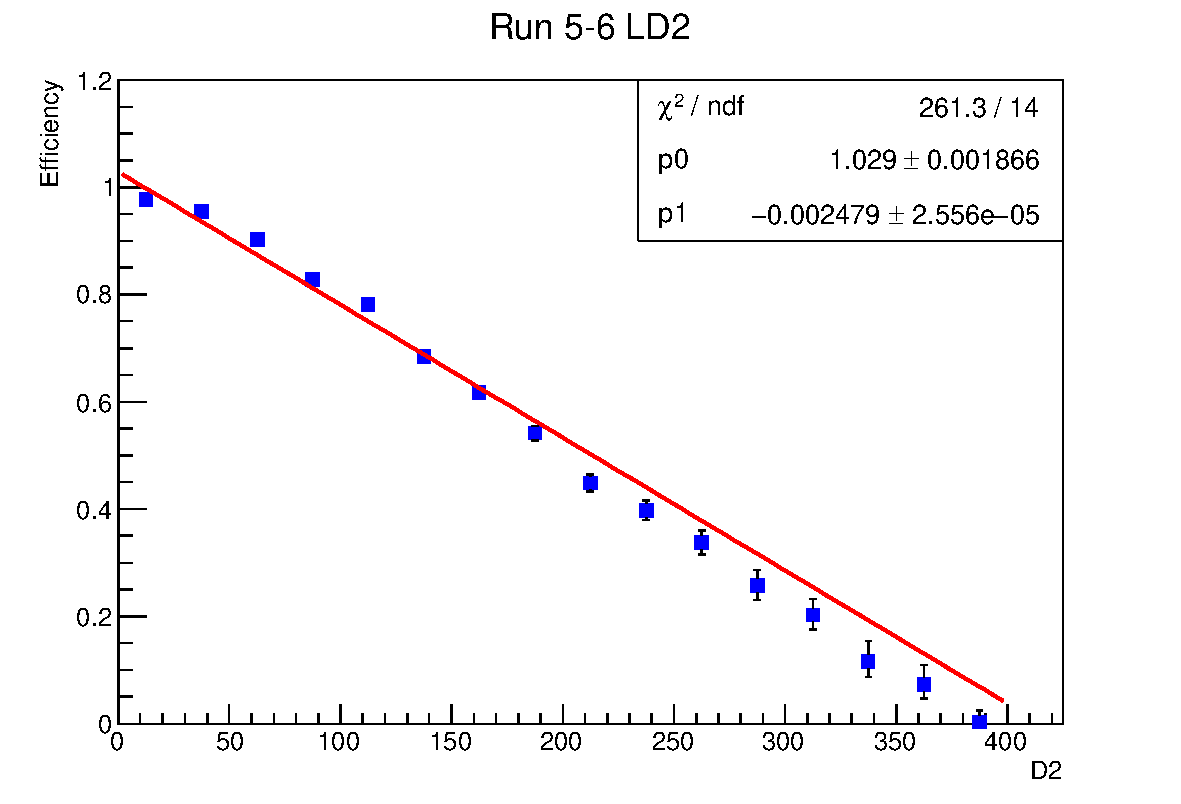
\includegraphics[width=0.5\linewidth]{run5-6_Drell-Yan_LD2}
	\caption{The reconstruction efficiency plotted as a function of station 2 occupancy, calculated using
		Run 5 \ce{LD_2} Drell-Yan MCs.
		The efficiency is calculated by taking the ratio of messy MC events over clean MC events in each
		occupancy bin. Standard cuts were applied to both numerator and denominator
		(except the occupancy cut on clean MC).
	}
	\label{fig:tracking efficiency}
\end{figure}
\pdfcomment{fit to messy/clean}

This tracking efficiency can also depends on the dimuon kinematics. This can be caused
by the noise hits are more localized in some area of the detector, which can mapped to
different kinematic phase space. To study this effect, we repeat the study with different
Monte Carlo, and the extract efficiency is shown in
\pdfcomment{table of efficiency for different target, process and runs}

Once the tracking efficiency obtained from the Monte Carlo, the efficiency correction ($\epsilon_{recon.Eff}$)
is calculated, which is defined as the average of the inverse of tracking efficiency in each
kinematic bin. This correction is calculated separately for each target, as a denser target
will produce more hits in the detector. This is shown in \cref{fig:target_D2}.

\begin{figure}[h!]
	\centering
	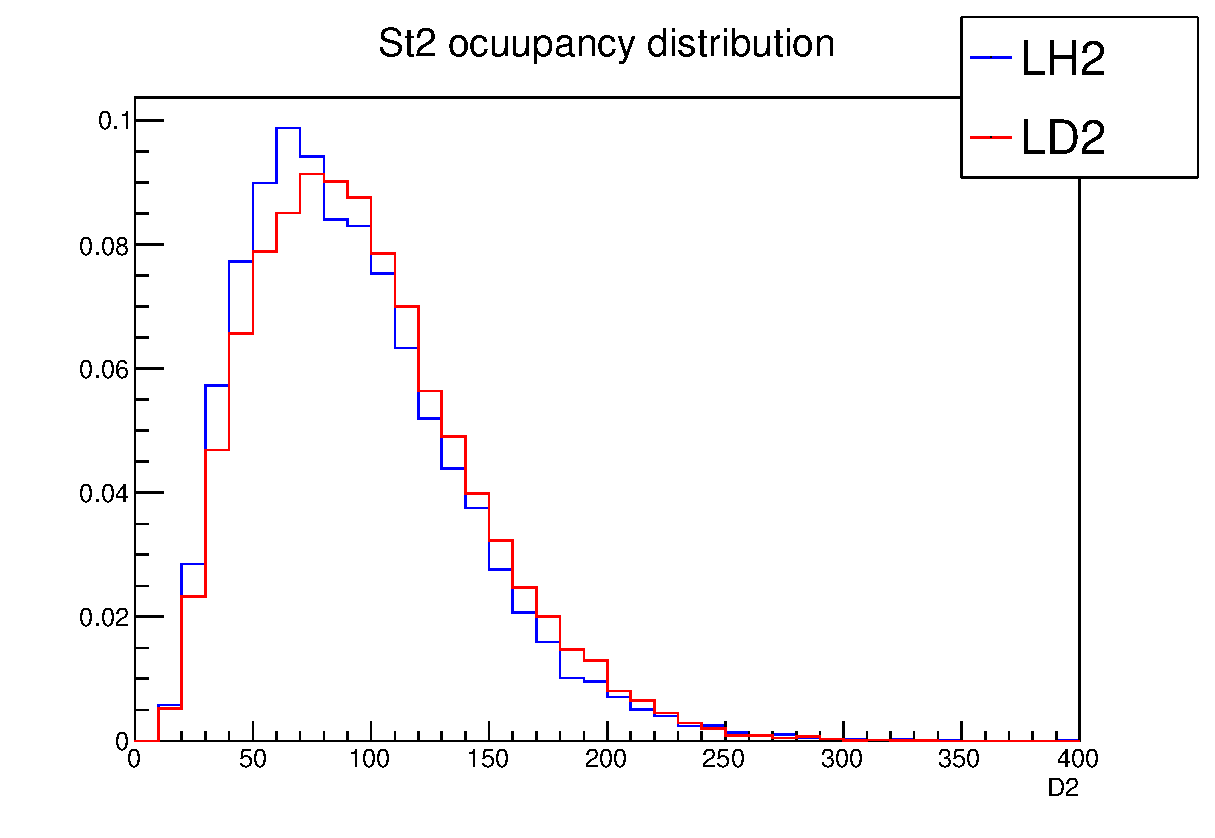
\includegraphics[width=0.5\linewidth]{run5-6_DY_D2}
	\caption{The St.~2 occupancy profile for \ce{LH_2} and \ce{LD_2} for run 5-6 after event selection. Both histogram are normalized to unit area.
	}
	\label{fig:target_D2}
\end{figure}
\pdfcomment{fig:target D2}

\section{Absolute \texorpdfstring{$J/\psi$}{J/psi} Cross Section Extraction}
\subsection{Target Contamination}
For a pure target, the cross section can be obtained from the yield using the following
\begin{equation}
	\sigma = \frac{Y A}{T N_A P X \epsilon},
\end{equation}
where $Y$ is the extracted yield, $A$ is the atomic mass of the target,
$T$ is the thickness of the target, $N_A$ is the Avogadro’s number,
$P$ is the proton on target, $\epsilon$ is the acceptance and efficiency correction,
and $X$ is the beam attenuation factor given by
\begin{equation}
	X=\frac{\lambda}{L\rho} \left[1-\exp\left(-\frac{L\rho}{\lambda}\right)\right],
\end{equation}
where $\lambda$ is the interaction length, $L$ and $\rho$ are the length and density
of the target.

The liquid targets are held in a flask \SI{50.8}{\cm} long and \SI{7.62}{\cm} in diameter
and can contain \SI{2.2}{\l} of liquid. The liquid Hydrogen used is \SI{99.999}{\percent}
pure. On the other hand, the Deuterium used came from two sources:
\begin{itemize}
	\item \SI{95.8\pm0.2}{\percent} pure deuterium that was used for bubble chamber experiments
	      at Fermilab, with contamination in the form of \ce{HD}.
	\item \SI{99.99}{\percent} pure commercial deuterium which is used in later part of the experiment.
\end{itemize}
\begin{table}[h!]
	\centering
	\caption{Summary of \ce{LD_2} contamination, taken from Ref.~\cite{don-4993}}
	\label{table:LD2_contamination}
	\begin{tabular}{|l|ll|l|l|}
		\hline
		Sample no. & \multicolumn{2}{l|}{\ce{D_2} bottle no.} & Sample date & description                                                                                                                          \\ \hline
		1          & \multicolumn{1}{l|}{Fermilab}            & 53          & 4/12/18     & \SI{95.6}{\percent} \ce{D}, \SI{4.4}{\percent} \ce{H}; \SI{92}{\percent}  \ce{D_2}, \SI{8}{\percent} \ce{HD} gases     \\
		2          & \multicolumn{1}{l|}{Fermilab}            & 113         & 4/12/18     & \SI{96}{\percent} \ce{D}, \SI{4}{\percent} \ce{H}; \SI{93}{\percent}  \ce{D_2}, \SI{7}{\percent} \ce{HD} gases         \\
		3          & \multicolumn{1}{l|}{Fermilab}            & 53          & 4/12/18     & just air; gas must have leaked                                                                                         \\
		4          & \multicolumn{1}{l|}{Matheson}            & 127         & 4/12/18     & about half air; remaining \SI{99.1}{\percent} \ce{D}, \SI{0.3}{\percent} \ce{H}                                        \\
		5          & \multicolumn{1}{l|}{Matheson}            & 2           & 4/12/18     & sample for test purposes; not analyzed                                                                                 \\
		6          & \multicolumn{1}{l|}{Matheson}            &             & 7/28/16     & more than half air; remaining \SI{99.3}{\percent} \ce{D}, \SI{0.7}{\percent} \ce{H}                                    \\
		7          & \multicolumn{1}{l|}{Matheson}            &             & 5/28/17     & \SI{99.8}{\percent} \ce{D}, \SI{0.2}{\percent} \ce{H}; \SI{99.6}{\percent}  \ce{D_2}, \SI{0.4}{\percent} \ce{HD} gases \\ \hline
	\end{tabular}
\end{table}
Therefore, care is needed to account for the contribution from the hydrogen contamination in deuterium
target data. The result of the mass spectroscopy of the deuterium gas \cite{don-4993} is
summarized in \cref{table:LD2_contamination}. Based this analysis, it is concluded the Fermilab
deuterium contains \SI{91.6}{\percent} \ce{D_2} and \SI{8.4}{\percent} \ce{HD} by moles. \pdfcomment{need to check this sentence.}

The yield from the contaminated deuterium can be expressed as
\begin{equation}
	Y_{\mathrm{cont.~\ce{LD_2}}} = N_A P_D X_D \epsilon_D \left( T_D^D \sigma_{pd}/A_D + T^D_H \sigma_{pp}/A_H   \right).
\end{equation}
Here $T_D^D$ and $T^D_H$ are the thickness of deuterium and hydrogen in the deuterium target.
The subscript $D$ denote these deuterium target specific quantities.

In order to extract the $T_D^D$ and $T^D_H$ from the mole fraction listed in \cref{table:LD2_contamination},
we first note that the volume of a \ce{HD} molecule is about \num{1.094} times the volume of a \ce{D_2}
molecule. Therefore the effective volume of molecules in the target is
\begin{equation}
	\begin{split}
		V_{\mathrm{eff.}}&=\frac{N_{\ce{HD}} V_{\ce{HD}} + N_{\ce{D_2}} V_{\ce{D_2}}}{N_{\text{tot.}}}\\
		&=V_{D_2} \left[ C \frac{V_{\ce{HD}}}{V_{\ce{D_2}}} + (1-C) \right]\\
		&=V_{D_2} f,
	\end{split}
\end{equation}
where $f=\left[ C \frac{V_{\ce{HD}}}{V_{\ce{D_2}}} + (1-C) \right]$.
The total number of molecules per area is
\begin{equation}
	\begin{split}
		\frac{N_{\mathrm{tot.}}}{\mathrm{Area}} &= \frac{L}{V_{\mathrm{eff.}}}\\
		&= \frac{L}{V_{\ce{D_2}}f}=\frac{L\rho_{\ce{D_2}}}{2A_Df}.
	\end{split}
\end{equation}
The thickness of D (in \unit{\g\per\cm\squared}) in the target cell is
\begin{equation}
	\begin{split}
		T_D^D &= \frac{N_D A_D}{\mathrm{Area}} = A_D\frac{N_{\mathrm{tot.}}}{\mathrm{Area}} \left[ 2(1-C) + C \right]\\
		&=A_D \frac{L\rho_{\ce{D_2}}}{2A_Df}(2-C)\\
		&=\frac{L\rho_{\ce{D_2}}}{f}(1-C/2).
	\end{split}
\end{equation}
The thickness of H (in \unit{\g\per\cm\squared}) in the target cell is
\begin{equation}
	\begin{split}
		T^D_H &= \frac{N_H A_H}{\mathrm{Area}} = A_H\frac{N_{\mathrm{tot.}}}{\mathrm{Area}}C\\
		&=\frac{L\rho_{\ce{D_2}}}{f}\frac{A_H}{A_D}\frac{C}{2}.
	\end{split}
	\label{eq:TDH}
\end{equation}
To determine the density of the deuterium target, the vent pressure is measured and is compared
with NIST database to obtained the expected density for pure deuterium ($\rho_{\ce{D_2}}$) \cite{density-1453}.
For contaminated deuterium, the effective density is
\begin{equation}
	\begin{split}
		\rho_{\mathrm{eff.}} &= \frac{1}{L} (T_D^H + T_D^D)\\
		&=\frac{\rho_{\ce{D_2}}}{f} \left[ \frac{A_H}{A_D}\frac{C}{2}+(1-C/2) \right].
	\end{split}
\end{equation}
and the effective interaction length is
\begin{equation}
	\begin{split}
		\frac{1}{\lambda_{\mathrm{eff.}}} &= \frac{1}{L\rho_{\mathrm{eff.}}} \left[\frac{T_D^H}{\lambda_H} +\frac{T_D^D}{\lambda_D}\right]\\
		&=\left[\frac{A_H}{A_D}\frac{C}{2\lambda_H} + \frac{1-C/2}{\lambda_D}\right]\left( \frac{A_H}{A_D}\frac{C}{2} +(1-C/2)\right)^{-1}.
	\end{split}
\end{equation}

Note that in previous studies and publication, including Ref.~\cite{dove2021}, the ratio of the atomic mass
is missing in \cref{eq:TDH}. This causes a roughly \SI{2}{\percent} difference in the cross section ratio
that will be discussed later.

Thus the deuterium cross section is
\begin{equation}
	\sigma_{pd} = \frac{Y_{\ce{LD_2}} A_D}{T_D^D N_A P_D X_{\mathrm{eff.}} \epsilon_D} - \frac{T^D_H}{T_D^D} \frac{A_D}{A_H} \sigma_{pp},
\end{equation}
where
\begin{equation}
	\sigma_{pp} = \frac{Y_{\ce{LH_2}} A_H}{T_H^H N_A P_D X_{H} \epsilon_H}.
\end{equation}
And the cross section ratio is given by
\begin{equation}
	\frac{\sigma_{pd}}{2\sigma_{pp}} = \frac{Y_{\ce{LD_2}}}{2Y_{\ce{LH_2}}}\frac{A_D}{A_H}\frac{T_H^H P_H X_{H} \epsilon_H}{T_D^D P_D X_{\mathrm{eff.}} \epsilon_D} - \frac{T^D_H}{2T_D^D} \frac{A_D}{A_H}.
\end{equation}

The switch to commercial pure deuterium gas happened during Roadset 67 data taking. Therefore,
an average contamination, weighted by the proton on target, is used for the entire dataset.
The average contamination for entire roadset 57 -70 data is determined to be $C=\SI{5.95}{\percent}$
Therefore the effective values for target contamination for this dataset are
\begin{equation}
	\begin{split}
		T_D^H &= \SI{0.1230}{\g\per\cm\squared}, \\
		T_D^D &= \SI{8.009}{\g\per\cm\squared},\\
		\rho_{\mathrm{eff.}} & = \SI{0.1601}{\g\per\cm\squared},\\
		\lambda_{\mathrm{eff.}} &= \SI{71.39}{\g\per\cm\squared},\\
		\lambda_{\mathrm{eff.}}/\rho_{\mathrm{eff.}} &= \SI{446.0}{\cm},\\
		X_{\mathrm{eff.}} &= 0.9451.
	\end{split}
\end{equation}
And since there is no contamination in the \ce{LH_2} target
\begin{equation}
	\begin{split}
		\rho_{H_2} &= \SI{0.0708}{\g\per\cm\cubed},\\
		T_H^H &= L\rho_{\ce{H_2}} = \SI{3.597}{\g\per\cm\squared},\\
		\lambda_H/\rho_{\ce{H_2}} &= \SI{734.5}{\cm},\\
		X_H &=0.9662.
	\end{split}
\end{equation}


\subsection{Acceptance Calculation}
The acceptance is obtained by comparing the clean Monte Carlo with thrown distribution,
and is defined as follows
\begin{equation}
	\epsilon_{acc.}\left(\Omega\right)=\mathrm{Acceptance}\left(\Omega\right)= \frac{N_{accept}\left(\Omega\right)}{N_{thrown}\left(\Omega\right)},
\end{equation}
where $N_{accept}\left(\Omega\right)$ is the number of accepted events in a given kinematic bin $\Omega$
by analyzing the clean Monte Carlo after passing the analysis procedure as the data, while $N_{thrown}$ is
the total number of generated Monte Carlo events in the same kinematic bin.

The accepted histogram in the numerator is filled using the reconstructed kinematic, whereas
the thrown histogram in the denominator is filled using the thrown kinematic.

Since our histogram are weighted histogram, the uncertainty is calculated using the following
\pdfcomment{verify the uncertainty calculation here}

\section{Comparison of data and Monte Carlo}

\subsection{\texorpdfstring{$P_T$}{P\_T} distribution}



\section{Systematic uncertainties}
For the Drell-Yan cross section ratios studies, the intensity extrapolation method and mass fit
method involve different assumption and therefore different sources of systematic uncertainties.
\paragraph{Proton beam normalization}
The beam normalization uncertainty is present in all studies presented here.
As described in \cref{sec:beam_norm}, the number of protons are measured by the BIM, which is
calibrated against a SEM monitor. The SEM monitor is further calibrated by studying the activation of
an irradiated high purity copper foil. A copper foil is placed in the beam line near the monitor,
causing the production of \ce{^{24}Na}. The \ce{^{24}Na} then decay into \ce{^{24}Mg} through $\beta$
decay. The number of  \ce{^{24}Na} nuclei is deduced by counting the number \SI{1369}{\keV} photons
produced. Using the \SI{3.56}{\milli\barn} production cross section for \ce{^{24}Na} in natural
copper  by \SI{120}{\GeV} protons, the number of incident protons can be deduced. The estimated
random uncertainty in the counting and extraction of \SI{1369}{\keV} peak is $\sim 1-2\%$.
An additional \SI{8}{\percent} systematic uncertainty in the production cross section of \ce{^{24}Na}
is also included \cite{docdb-457,docdb-7708}.
A total of \SI{10}{\percent} beam normalization uncertainty is assigned to absolute cross
section studies, whereas a \SI{2}{\percent} relative normalization uncertainty is assigned to ratios between
targets. This \SI{2}{\percent} relative normalization uncertainty is also included in the empty flask
subtraction.

\paragraph{Choice of fit function}
This is specific to the cross section ratio studies using intensity extrapolation method.
To estimate the effect of the choice of fit function, different fit functions were examined.
For example, we can allow the $p_1$ and $p_2$ parameters in \cref{eq:common_pol2} to have kinematic
dependence
\begin{equation}
	R_i \left(I\right) = p_{0i} + \left[p_{10}+p_{11}x_i\right] I + \left[p_{20}+p_{21}x_i\right] I^2,
\end{equation}
where $x_i$ is the kinematic average in each bin. The difference between the fit functions are used
as the systematic uncertainty.

\paragraph{Mixed background}
This is specific to studies using mass fit method. Different mixing methods have been proposed in SeaQuest.
The mixed sample from the two methods described in \cref{sec:mixing} are studied. The difference between 
the two analysis in included in the systematic uncertainty.

\paragraph{Acceptance simulation}
This is a major systematics in the absolute cross section studies, particularly when using
Run 2-3 data.
During Run 2-3, multiple trigger road sets were used. However, due to the limited statistics in each
data taking period, it is not possible to analysis each subset separately. Therefore these datasets
are combined into one. While the difference in trigger road set have little effect on the acceptance
for the high mass Drell-Yan dimuon \cite{jdove-8168}, the impact on the $J/\psi$ acceptance is much
larger \cite{chleung-9643}.

During later runs, only one trigger road set (roadset 78) was used, hence this is no
longer an issue.



\section{Drell-Yan NLO calculation}
The next-to-leading order (NLO) calculation is done using a parton level Monte
Carlo program written by the INFN group\cite{catani2009,catani2007}. This program
is originally written to compute written to compute cross-section for vector boson
production from $p+p$ and $p+\bar{p}$ collisions. It was later modified, in
collaboration with Wen-Chen Chang and Shivangi Prasad, to perform $p+n$ calculation
by utilizing isospin symmetry. The $p+d$ interaction can be computed by summing up
the $p+p$ and $p+n$ calculation, assuming no nuclear corrections. For heavier nuclear
targets, nuclear PDFs can also be used.

\pdfmargincomment{Error calculations}
The PDF sets used in this study are CT18\cite{hou2019} and NNPDF4.0\cite{ball2021}.
And they are accessed through the LHAPDF library\cite{buckley2015}. It should be noted
that the CT18 PDF set is published before the SeaQuest result, whereas NNPDF4.0
incorporate the SeaQuest measurements\cite{dove2021} in the global fit.

The uncertainty band for calculations using CT18 PDFs are calculated using the hessian methods.
Given a central PDF member $S_0$ and $2N_{\mathrm{par}}$ eigenvector PDF member $S^\pm_i$ ($i=1,\dots,N_{\mathrm{par}}$),
where $N_{\mathrm{par}}$ is the number of parameters. The central value $F_0$ and the uncertainty $\sigma^\pm_F$
on a PDF-dependent quantity are given by:
\begin{equation}
	\begin{split}
		F_0 &= F(S_0),\quad F_i^\pm=F(S_i^\pm) \\
		\sigma^+_F &= \sqrt{\sum_{i=1}^{N_{\mathrm{par}}} \left[\max\left(F_i^+ - F_0, F_0 - F^-_i,0\right)\right]^2 }\\
		\sigma^-_F &= \sqrt{\sum_{i=1}^{N_{\mathrm{par}}} \left[\max\left(F_0 - F^+_i, F_i^- - F_0,0\right)\right]^2 }
	\end{split}
\end{equation}

Whereas the uncertainty for NNPDF4.0 is calculated using the replicas method. Given $N_{\mathrm{rep}}$ replica
PDF members $S^k$, the central value and the uncertainty is given by the mean and standard distribution
\begin{equation}
	\begin{split}
		F_0&=\expval{F}=\frac{1}{N_{\mathrm{rep}}}\sum_{i=1}^{N_{\mathrm{rep}}}F\left(S^k\right)\\
		\sigma_F&= \sqrt{\frac{1}{N_{\mathrm{rep}}-1}\sum_{i=1}^{N_{\mathrm{rep}}}\left[F\left(S^k\right)-F_0\right]^2}
	\end{split}
\end{equation}

It should also be noted that CT18 reports the \SI{90}{\percent} confidence level by default, whereas NNPDF4.0
would report the \SI{68}{\percent} confidence level.

\ifSubfilesClassLoaded{ \printbibliography[heading=bibintoc,title={References}]}{}
\end{document}


\chapter{Results}
\label{ch:tesult}
\documentclass[../main.tex]{subfiles}
\begin{document}

\ifSubfilesClassLoaded{
	\mainmatter
	\setcounter{chapter}{5}
}{}

\chapter{Results}
\label{ch:result}
\section{Drell-Yan Cross Section Ratio}
\subsection{Results from Run 2-3 data}
\subsubsection{Effect of the updated target contamination correction}
\label{subsubsec:contamination_result}
As discussed in \cref{M-subsec:contamination}, an incorrect target contamination correction was used
in previous publications and the effect is shown in \cref{fig:contaimination_CSR}.
The overall effect is a roughly \SI{2}{\percent} shift in the ratio.
\begin{figure}[h!]
	\centering
	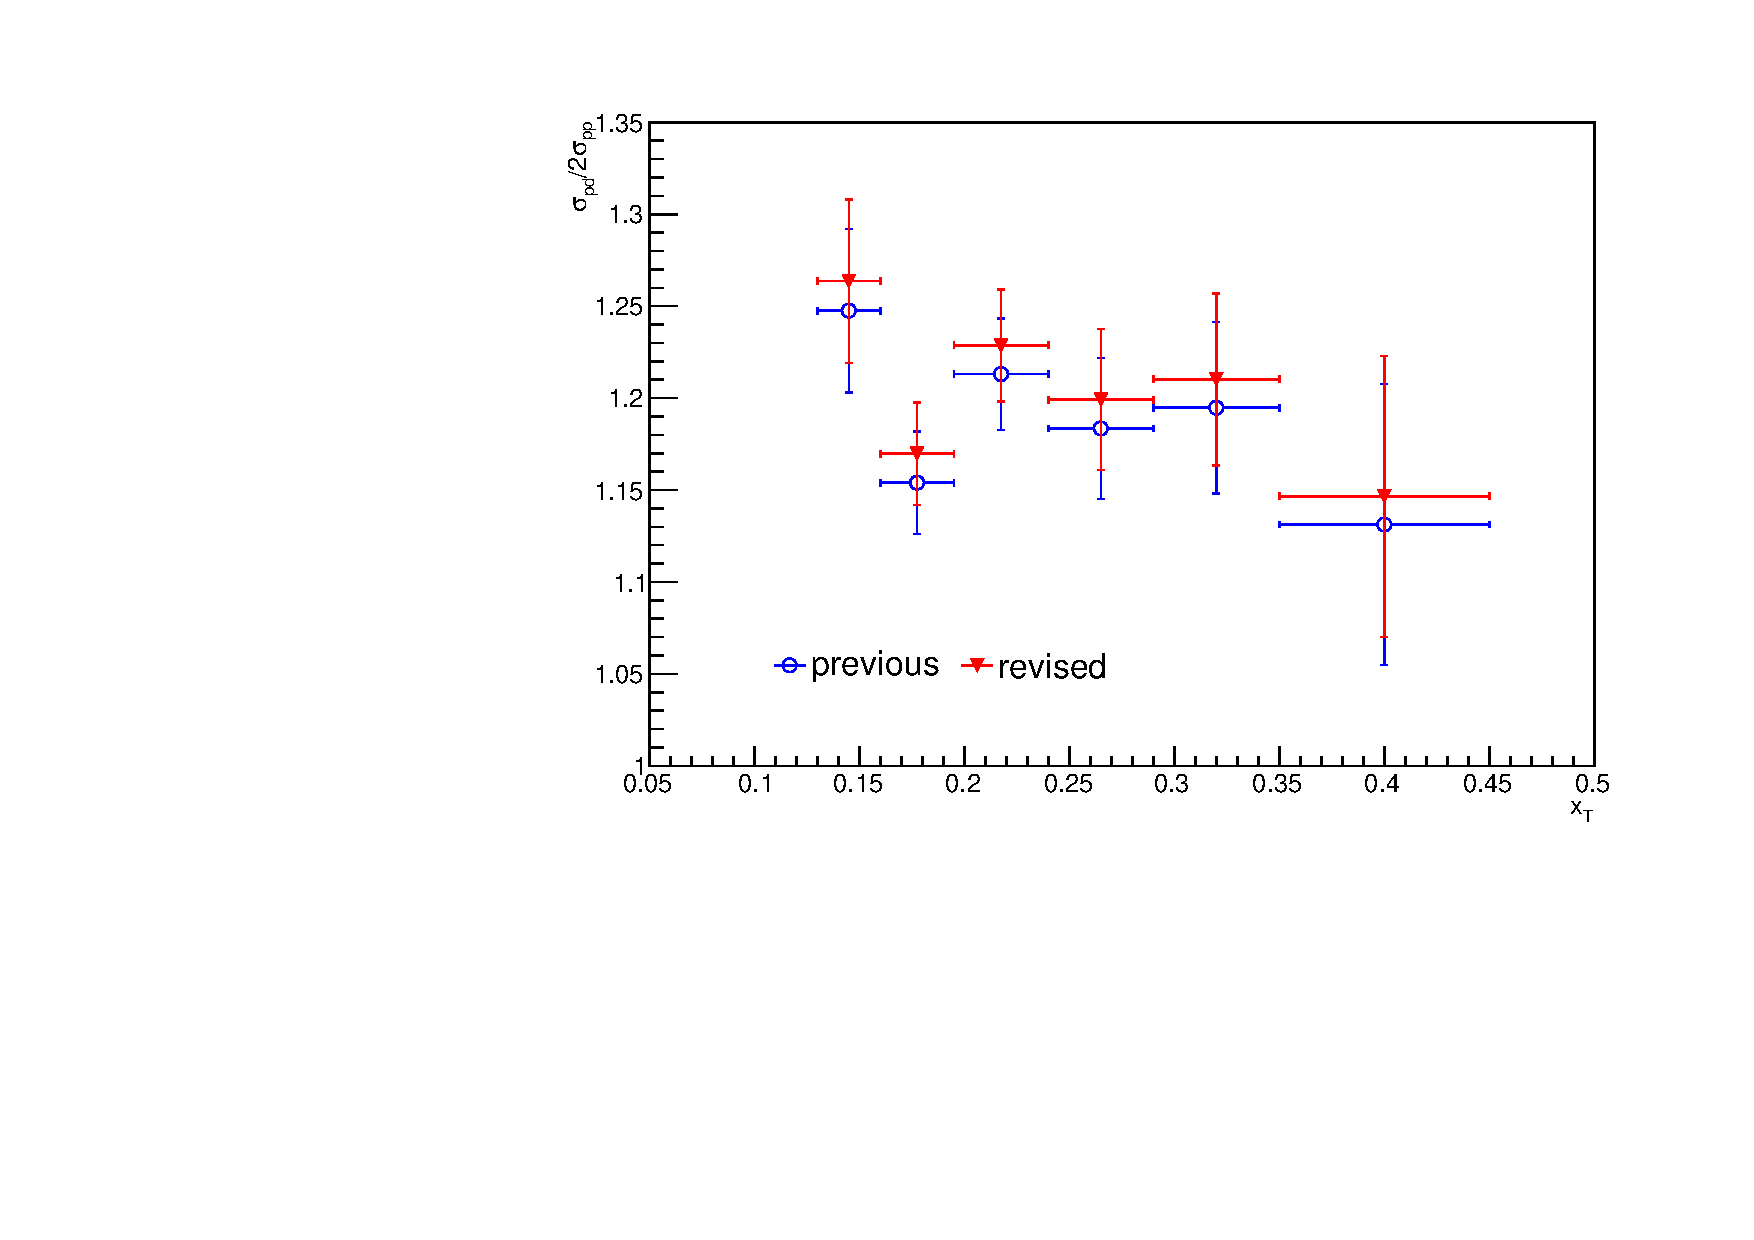
\includegraphics[width=0.6\linewidth]{DY-csr/Compare_targetCorr}
	\caption{The effect of the updated target contamination correction on the Drell-Y.an
		cross section. The extracted cross section ratio using the revised target contamination
		is shown as red sold triangle, and the previous published version is shown as blue open
		circle. The overall effect is a roughly \SI{2}{\percent} shift in the ratio. }
	\label{fig:contaimination_CSR}
\end{figure}



\subsubsection{Choice of fit function in intensity extrapolation}
To understand the systematic uncertainties in the intensity extrapolation method due to the
choice of fit function, the following functions are used.
\begin{align}
	R_i\left(I\right) & = p_{0i} + p_{1} I + p_{2} I^2 \quad\text{(FIT 1)}                                                     \\
	R_i\left(I\right) & = p_{0i} + \left[p_{10} + p_{11}x_i\right] I + \left[p_{20} + p_{21}x_i\right]I^2 \quad \text{(FIT 2)}
\end{align}
The fit to data using the two fits are shown in \cref{fig:run2-3_FIT1_xT,fig:run2-3_FIT2_xT}
and $\chi^2$ for the fits are tabulated in \cref{tab:chi_run23}.
And the fit for other variables are listed in \cref{M-a_ch:extrapolation}.
\begin{figure}
	\centering
	\caption{Fit to the flask subtracted yield ratio with FIT1 for $x_T$ for run 2-3.}
	\label{fig:run2-3_FIT1_xT}
	\begin{subfigure}{0.45\linewidth}
		\includegraphics[width=\linewidth]{extrapolation/run2-3/xT/FIT1/hist_fitted_xT_tInt_0}
	\end{subfigure}
	\begin{subfigure}{0.45\linewidth}
		\includegraphics[width=\linewidth]{extrapolation/run2-3/xT/FIT1/hist_fitted_xT_tInt_1}
	\end{subfigure}
	\begin{subfigure}{0.45\linewidth}
		\includegraphics[width=\linewidth]{extrapolation/run2-3/xT/FIT1/hist_fitted_xT_tInt_2}
	\end{subfigure}
	\begin{subfigure}{0.45\linewidth}
		\includegraphics[width=\linewidth]{extrapolation/run2-3/xT/FIT1/hist_fitted_xT_tInt_3}
	\end{subfigure}
	\begin{subfigure}{0.45\linewidth}
		\includegraphics[width=\linewidth]{extrapolation/run2-3/xT/FIT1/hist_fitted_xT_tInt_4}
	\end{subfigure}
	\begin{subfigure}{0.45\linewidth}
		\includegraphics[width=\linewidth]{extrapolation/run2-3/xT/FIT1/hist_fitted_xT_tInt_5}
	\end{subfigure}
\end{figure}

\begin{figure}
	\centering
	\caption{Fit to the flask subtracted yield ratio with FIT2 for $x_T$ for run 2-3.}
	\label{fig:run2-3_FIT2_xT}
	\begin{subfigure}{0.45\linewidth}
		\includegraphics[width=\linewidth]{extrapolation/run2-3/xT/FIT2/hist_fitted_xT_tInt_0}
	\end{subfigure}
	\begin{subfigure}{0.45\linewidth}
		\includegraphics[width=\linewidth]{extrapolation/run2-3/xT/FIT2/hist_fitted_xT_tInt_1}
	\end{subfigure}
	\begin{subfigure}{0.45\linewidth}
		\includegraphics[width=\linewidth]{extrapolation/run2-3/xT/FIT2/hist_fitted_xT_tInt_2}
	\end{subfigure}
	\begin{subfigure}{0.45\linewidth}
		\includegraphics[width=\linewidth]{extrapolation/run2-3/xT/FIT2/hist_fitted_xT_tInt_3}
	\end{subfigure}
	\begin{subfigure}{0.45\linewidth}
		\includegraphics[width=\linewidth]{extrapolation/run2-3/xT/FIT2/hist_fitted_xT_tInt_4}
	\end{subfigure}
	\begin{subfigure}{0.45\linewidth}
		\includegraphics[width=\linewidth]{extrapolation/run2-3/xT/FIT2/hist_fitted_xT_tInt_5}
	\end{subfigure}
\end{figure}



\Cref{fig:CSR_Run2-3} shows the extracted cross section ratio as a function of $x_T$, $x_B$ and $x_F$.
While the two fit functions produce similar results for $x_T$, the differences are larger in
the other variables.

\begin{figure}[h!]
	\centering
	\begin{subfigure}{0.6\linewidth}
		\includegraphics*[width=\linewidth]{DY-csr/run23-xT_all}
	\end{subfigure}\\
	\begin{subfigure}{0.45\linewidth}
		\includegraphics*[width=\linewidth]{DY-csr/run23-xB_all}
	\end{subfigure}
	\begin{subfigure}{0.45\linewidth}
		\includegraphics*[width=\linewidth]{DY-csr/run23-xF_all}
	\end{subfigure}
	\caption{Comparison of the extracted Drell-Yan cross section ratio as a function of $x_T$(top),
		$x_B$(left) and $x_F$(right) using the different methods from the Run 2-3
		data.}
	\label{fig:CSR_Run2-3}
\end{figure}

\begin{table}[h!]
	\centering
	\caption{The reduced $\chi^2$ for the different fits used in the intensity extrapolation method for Run 2-3. }
	\label{tab:chi_run23}
	\begin{tabular}{|l|lll|}
\hline
 & \multicolumn{3}{c|}{$\chi^2/NDF$} \\ \cline{2-4} 
      & \multicolumn{1}{c|}{$x_T$}          & \multicolumn{1}{c|}{$x_B$}          & \multicolumn{1}{c|}{$x_F$} \\ \hline
FIT 1 & \multicolumn{1}{l|}{$40.1167 / 40$} & \multicolumn{1}{l|}{$71.3796 / 47$} & $68.0593 / 47$             \\ \hline
FIT 2 & \multicolumn{1}{l|}{$40.008 / 38$}  & \multicolumn{1}{l|}{$61.8549 / 45$} & $64.1524 / 45$             \\ \hline
\end{tabular}

\end{table}


\subsubsection{Comparison of massfit and extrapolation}
\Cref{fig:massfit_integrated_run23} shows the fit to the mass distributions for Run 2-3 data, and the
data is very well described by the fitting procedure.
\begin{figure}[h!]
	\begin{subfigure}{0.45\linewidth}
		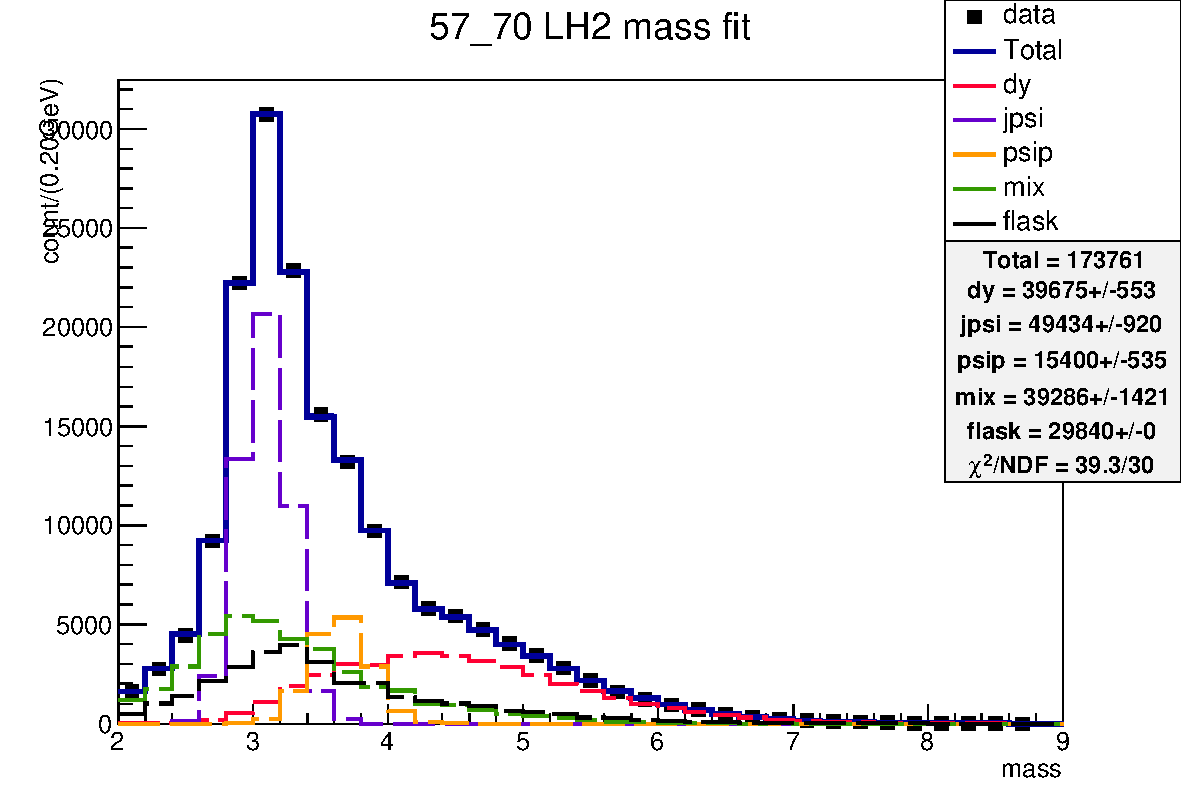
\includegraphics[width=\linewidth]{massfit/run2-3/57_70_LH2}
	\end{subfigure}
	\begin{subfigure}{0.45\linewidth}
		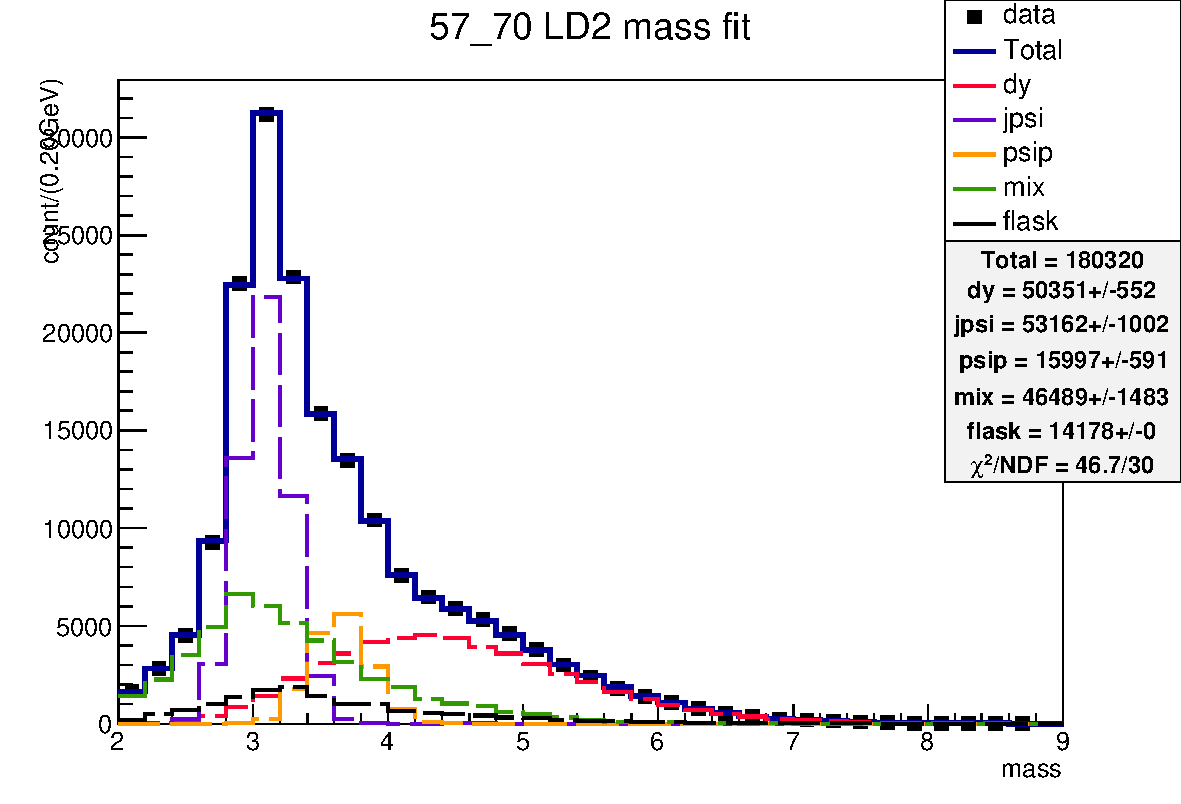
\includegraphics[width=\linewidth]{massfit/run2-3/57_70_LD2}
	\end{subfigure}
	\caption{The mass spectrum for \ce{LH_2}(left) and \ce{LD_2}(right) targets data for Run 2-3}
	\label{fig:massfit_integrated_run23}
\end{figure}

With the yield for different process obtained from the mass fits, the cross section ratios can be calculated
and are also shown in \cref{fig:CSR_Run2-3}.
As reported in Ref.~\cite{dove2023} the Drell-Yan cross section ratio as a function of $x_T$ extracted from
the two methods are in very good agreement.

However, the comparison in other variables, such as $x_B$ and $x_F$ are complicated by the large
systematical uncertainties originated from the fit function used in the intensity extrapolation.
\Cref{fig:CSR_Run2-3} shows the extracted ratios as a function of $x_B$ and $x_F$ using different methods.
While the massfit results agree with the extrapolation result if FIT 1 is used, the
extrapolation results using FIT 2 are different from the other two.

\FloatBarrier

\subsection{Results from Run 5-6 data}
\begin{figure}[h!]
	\begin{subfigure}{0.45\linewidth}
		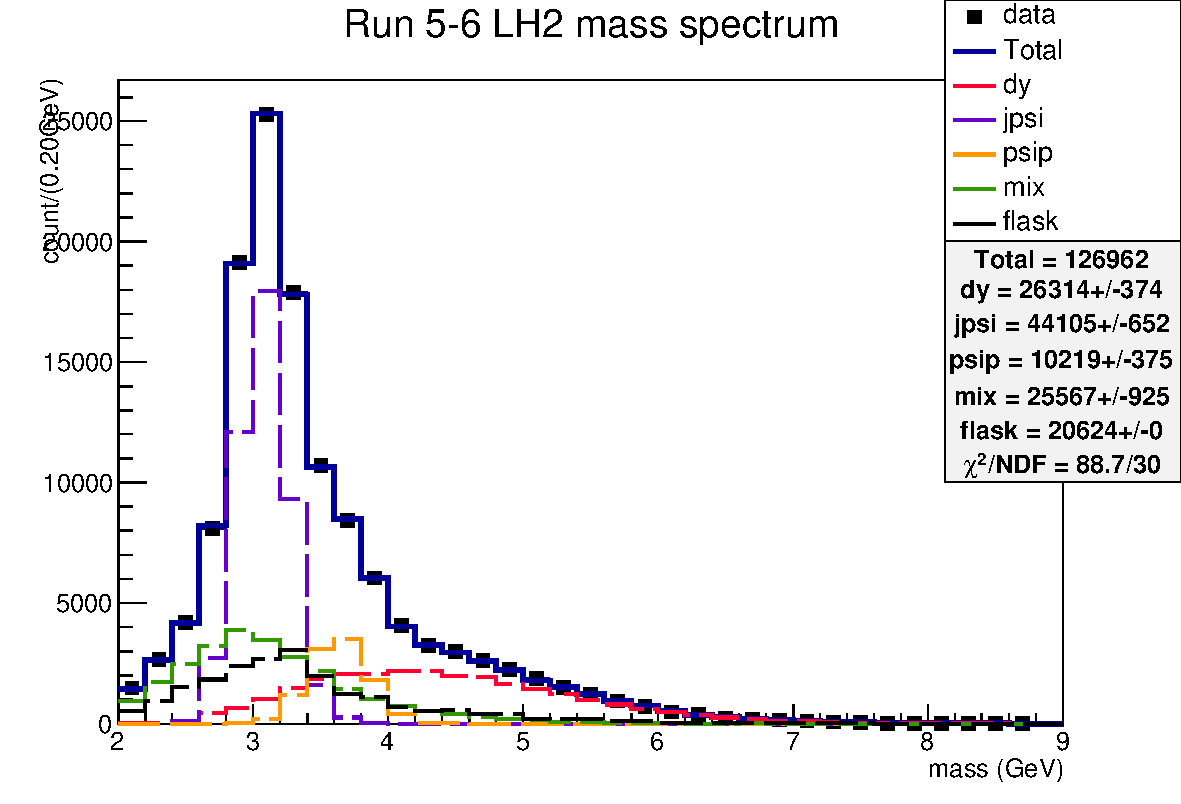
\includegraphics[width=\linewidth]{massfit/run5-6/5_6_LH2}
	\end{subfigure}
	\begin{subfigure}{0.45\linewidth}
		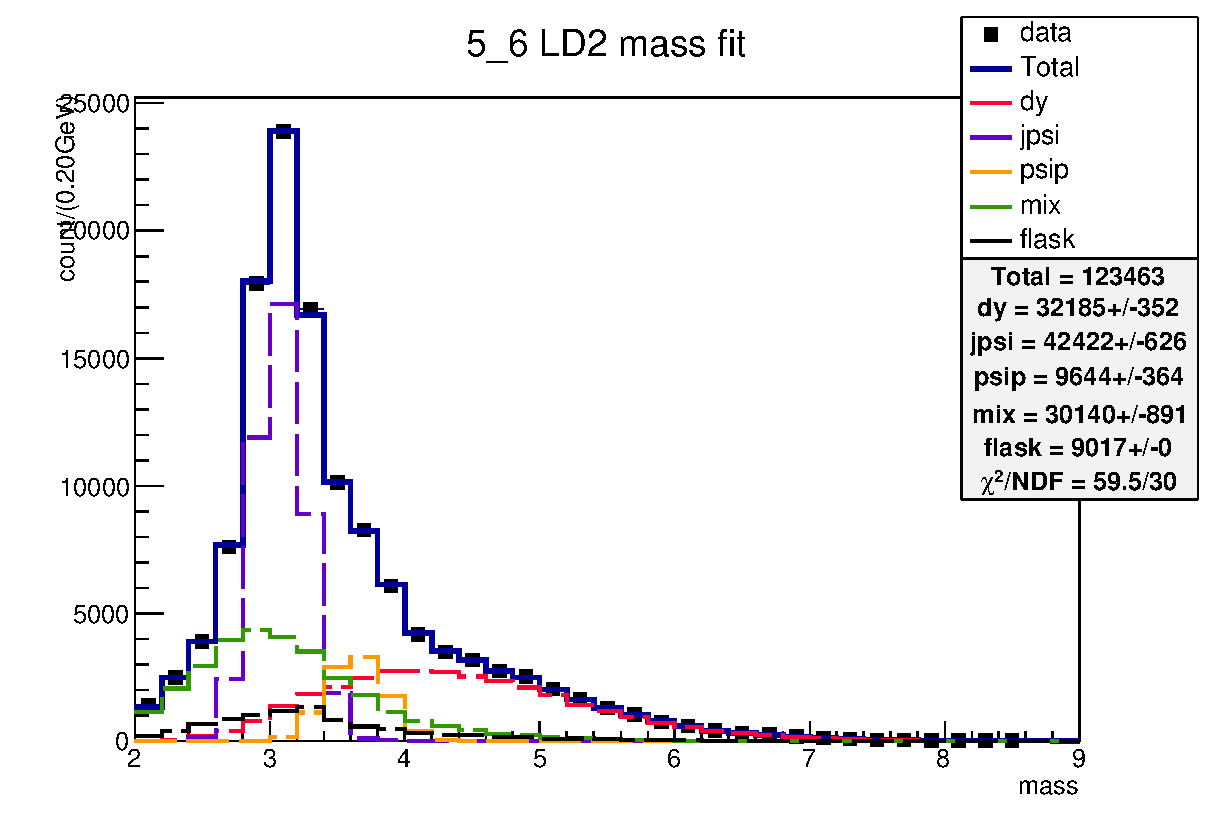
\includegraphics[width=\linewidth]{massfit/run5-6/5_6_LD2}
	\end{subfigure}
	\caption{The mass spectrum for \ce{LH_2}(left) and \ce{LD_2}(right) targets data for Run 5-6}
	\label{fig:massfit_integrated_run56}
\end{figure}

\begin{figure}
\begin{subfigure}{0.45\linewidth}
\includegraphics{width=\linewidth}{extrapolation/run5-6/xT/FIT1/hist_fitted_xT_tInt_0}
\end{subfigure}
\begin{subfigure}{0.45\linewidth}
\includegraphics{width=\linewidth}{extrapolation/run5-6/xT/FIT1/hist_fitted_xT_tInt_1}
\end{subfigure}
\begin{subfigure}{0.45\linewidth}
\includegraphics{width=\linewidth}{extrapolation/run5-6/xT/FIT1/hist_fitted_xT_tInt_2}
\end{subfigure}
\begin{subfigure}{0.45\linewidth}
\includegraphics{width=\linewidth}{extrapolation/run5-6/xT/FIT1/hist_fitted_xT_tInt_3}
\end{subfigure}
\begin{subfigure}{0.45\linewidth}
\includegraphics{width=\linewidth}{extrapolation/run5-6/xT/FIT1/hist_fitted_xT_tInt_4}
\end{subfigure}
\begin{subfigure}{0.45\linewidth}
\includegraphics{width=\linewidth}{extrapolation/run5-6/xT/FIT1/hist_fitted_xT_tInt_5}
\end{subfigure}
\end{figure}

\begin{figure}
	\centering
	\caption{Fit to the flask subtracted yield ratio with FIT2 for $x_T$ for run 5-6.}
	\label{fig:run5-6_FIT2_xT}
	\begin{subfigure}{0.45\linewidth}
		\includegraphics[width=\linewidth]{extrapolation/run5-6/xT/FIT2/hist_fitted_xT_tInt_0}
	\end{subfigure}
	\begin{subfigure}{0.45\linewidth}
		\includegraphics[width=\linewidth]{extrapolation/run5-6/xT/FIT2/hist_fitted_xT_tInt_1}
	\end{subfigure}
	\begin{subfigure}{0.45\linewidth}
		\includegraphics[width=\linewidth]{extrapolation/run5-6/xT/FIT2/hist_fitted_xT_tInt_2}
	\end{subfigure}
	\begin{subfigure}{0.45\linewidth}
		\includegraphics[width=\linewidth]{extrapolation/run5-6/xT/FIT2/hist_fitted_xT_tInt_3}
	\end{subfigure}
	\begin{subfigure}{0.45\linewidth}
		\includegraphics[width=\linewidth]{extrapolation/run5-6/xT/FIT2/hist_fitted_xT_tInt_4}
	\end{subfigure}
	\begin{subfigure}{0.45\linewidth}
		\includegraphics[width=\linewidth]{extrapolation/run5-6/xT/FIT2/hist_fitted_xT_tInt_5}
	\end{subfigure}
\end{figure}


\pdfmargincomment{run 5-6 compared with 2-3 and full data set, only show massfit results?}
\Cref{fig:CSR_Run5-6} shows the extracted cross section ratio as a function from the
second half of our data using various methods. While the different fit functions used in the
intensity extrapolation produce very similar results, the massfit result is significantly larger
than the intensity extrapolation results.
\begin{figure}[h!]
	\centering
	\begin{subfigure}{0.6\linewidth}
		\includegraphics*[width=\linewidth]{DY-csr/run56-xT_all}
	\end{subfigure}
	\begin{subfigure}{0.45\linewidth}
		\includegraphics*[width=\linewidth]{DY-csr/run56-xB_all}
	\end{subfigure}
	\begin{subfigure}{0.45\linewidth}
		\includegraphics*[width=\linewidth]{DY-csr/run56-xF_all}
	\end{subfigure}
	\caption{Comparison of the extracted Drell-Yan cross section ratio as a function of $x_T$(top),  $x_B$(left)
		and $x_F$(right) from the Run 5-6 data using the massfit and intensity extrapolation method.}
	\label{fig:CSR_Run5-6}
\end{figure}
\begin{table}
	\centering
	\caption{The reduced $\chi^2$ for the different fits used in the intensity extrapolation method for Run 5-6. }
	\label{tab:chi_run56}
	\begin{tabular}{|l|lll|}
\hline
 & \multicolumn{3}{c|}{$\chi^2/NDF$} \\ \cline{2-4} 
      & \multicolumn{1}{c|}{$x_T$}          & \multicolumn{1}{c|}{$x_B$}          & \multicolumn{1}{c|}{$x_F$} \\ \hline
FIT 1 & \multicolumn{1}{l|}{$24.3236 / 28$} & \multicolumn{1}{l|}{$41.6412 / 33$} & $28.1757 / 33$             \\ \hline
FIT 2 & \multicolumn{1}{l|}{$23.2091 / 26$}  & \multicolumn{1}{l|}{$40.3455 / 31$} & $25.7949 / 31$             \\ \hline
\end{tabular}

\end{table}

\subsubsection{Potential cause of difference between massfit and intensity extrapolation}
During the second half of the data taking, the variation in the instantaneous beam
intensity was reduced as compared to run 2-3. This is partly due to the improvement
in beam quality and partly due to the tightening of the beam inhibit thresholds.

The massfit and intensity extrapolation methods made different assumption on the intensity
and rate dependence. With less high intensity data, there are less constraints on the
intensity dependence, causing the two method to disagree.

\pdfcomment{Intensity range cannot explain the discrepancy }

\subsection{Comparison with global PDF analysis}
\pdfmargincomment{modified to impact of SeaQuest result?}
The published $\sigma_{pd}/2\sigma_{pp}$ ratio result has been included in various recent global
PDF analysis, including Ref.~\cite{cocuzza2021,guzzi2022,accardi2023,alekhin2023}.
In particular, \cref{fig:CSR_Run2-3} shows the calculation using CT18 (without the SeaQuest data)
and NNPDF 4.0 (including the SeaQuest data). The shift in the cross section ratio is primarily
coming from the inclusion of the SeaQuest data. Unlike the previous E866 result, the SeaQuest data
strongly suggests the $\bar{d}/\bar{u}$ ratio would remain greater than one for $x<0.4$, which is
consistent with prediction from various models, including meson cloud and statistical model.

The importance of the SeaQuest data can be seen in the NNPDF 4.0, where at large $x_T$,
uncertainties bands is consistent with the uncertainties of our measurements, as the SeaQuest
results is the only available data sensitive to the light sea-quark asymmetry at large $x$.
\FloatBarrier

\section{Charmonium Cross Section}

\subsection{Massfit results}
The massfits in all $x_F$ bins are shown in \cref{fig:massfit_57-70_xF,fig:massfit_5-6_xF},
and the fits in the $P_T$ bins are shown in \cref{fig:massfit_57-70_pT,fig:massfit_5-6_pT}.
The two datasets are analyzed separately. The data in each bin is very well described by the fitting procedure
and the $J/\psi$ and $\psi'$ yields can be extracted from the fits directly.
\pdfmargincomment{undate massfit plots!!!}
\begin{figure}[h]
	\centering
	\begin{subfigure}{0.4\linewidth}
		\includegraphics[width=0.9\linewidth]{massfit/run2-3/LH2/xF/LH2_xFbin0}
	\end{subfigure}
	\begin{subfigure}{0.4\linewidth}
		\includegraphics[width=0.9\linewidth]{massfit/run2-3/LD2/xF/LD2_xFbin0}
	\end{subfigure}\\
	\begin{subfigure}{0.4\linewidth}
		\includegraphics[width=0.9\linewidth]{massfit/run2-3/LH2/xF/LH2_xFbin1}
	\end{subfigure}
	\begin{subfigure}{0.4\linewidth}
		\includegraphics[width=0.9\linewidth]{massfit/run2-3/LD2/xF/LD2_xFbin1}
	\end{subfigure}\\
	\begin{subfigure}{0.4\linewidth}
		\includegraphics[width=0.9\linewidth]{massfit/run2-3/LH2/xF/LH2_xFbin2}
	\end{subfigure}
	\begin{subfigure}{0.4\linewidth}
		\includegraphics[width=0.9\linewidth]{massfit/run2-3/LD2/xF/LD2_xFbin2}
	\end{subfigure}\\
	\begin{subfigure}{0.4\linewidth}
		\includegraphics[width=0.9\linewidth]{massfit/run2-3/LH2/xF/LH2_xFbin3}
	\end{subfigure}
	\begin{subfigure}{0.4\linewidth}
		\includegraphics[width=0.9\linewidth]{massfit/run2-3/LD2/xF/LD2_xFbin3}
	\end{subfigure}\\
	\begin{subfigure}{0.4\linewidth}
		\includegraphics[width=0.9\linewidth]{massfit/run2-3/LH2/xF/LH2_xFbin4}
	\end{subfigure}
	\begin{subfigure}{0.4\linewidth}
		\includegraphics[width=0.9\linewidth]{massfit/run2-3/LD2/xF/LD2_xFbin4}
	\end{subfigure}
	\caption{Mass fit for run 2-3 data in each $x_F$ bin for both \ce{LH_2}(left) and \ce{LD_2}(right) targets. }
	\label{fig:massfit_57-70_xF}
\end{figure}

\begin{figure}[h]
	\centering
	\begin{subfigure}{0.4\linewidth}
		\includegraphics[width=0.9\linewidth]{massfit/run5-6/LH2/xF/LH2_xFbin0}
	\end{subfigure}
	\begin{subfigure}{0.4\linewidth}
		\includegraphics[width=0.9\linewidth]{massfit/run5-6/LD2/xF/LD2_xFbin0}
	\end{subfigure}\\
	\begin{subfigure}{0.4\linewidth}
		\includegraphics[width=0.9\linewidth]{massfit/run5-6/LH2/xF/LH2_xFbin1}
	\end{subfigure}
	\begin{subfigure}{0.4\linewidth}
		\includegraphics[width=0.9\linewidth]{massfit/run5-6/LD2/xF/LD2_xFbin1}
	\end{subfigure}\\
	\begin{subfigure}{0.4\linewidth}
		\includegraphics[width=0.9\linewidth]{massfit/run5-6/LH2/xF/LH2_xFbin2}
	\end{subfigure}
	\begin{subfigure}{0.4\linewidth}
		\includegraphics[width=0.9\linewidth]{massfit/run5-6/LD2/xF/LD2_xFbin2}
	\end{subfigure}\\
	\begin{subfigure}{0.4\linewidth}
		\includegraphics[width=0.9\linewidth]{massfit/run5-6/LH2/xF/LH2_xFbin3}
	\end{subfigure}
	\begin{subfigure}{0.4\linewidth}
		\includegraphics[width=0.9\linewidth]{massfit/run5-6/LD2/xF/LD2_xFbin3}
	\end{subfigure}\\
	\begin{subfigure}{0.4\linewidth}
		\includegraphics[width=0.9\linewidth]{massfit/run5-6/LH2/xF/LH2_xFbin4}
	\end{subfigure}
	\begin{subfigure}{0.4\linewidth}
		\includegraphics[width=0.9\linewidth]{massfit/run5-6/LD2/xF/LD2_xFbin4}
	\end{subfigure}
	\caption{Mass fit for run 5-6 data in each $x_F$ bin for both \ce{LH_2}(left) and \ce{LD_2}(right) targets. }
	\label{fig:massfit_5-6_xF}
\end{figure}

\begin{figure}[h]
	\centering
	\begin{subfigure}{0.4\linewidth}
		\includegraphics[width=0.9\linewidth]{massfit/run2-3/LH2/pT/LH2_pTbin0}
	\end{subfigure}
	\begin{subfigure}{0.4\linewidth}
		\includegraphics[width=0.9\linewidth]{massfit/run2-3/LD2/pT/LD2_pTbin0}
	\end{subfigure}\\
	\begin{subfigure}{0.4\linewidth}
		\includegraphics[width=0.9\linewidth]{massfit/run2-3/LH2/pT/LH2_pTbin1}
	\end{subfigure}
	\begin{subfigure}{0.4\linewidth}
		\includegraphics[width=0.9\linewidth]{massfit/run2-3/LD2/pT/LD2_pTbin1}
	\end{subfigure}\\
	\begin{subfigure}{0.4\linewidth}
		\includegraphics[width=0.9\linewidth]{massfit/run2-3/LH2/pT/LH2_pTbin2}
	\end{subfigure}
	\begin{subfigure}{0.4\linewidth}
		\includegraphics[width=0.9\linewidth]{massfit/run2-3/LD2/pT/LD2_pTbin2}
	\end{subfigure}\\
	\begin{subfigure}{0.4\linewidth}
		\includegraphics[width=0.9\linewidth]{massfit/run2-3/LH2/pT/LH2_pTbin3}
	\end{subfigure}
	\begin{subfigure}{0.4\linewidth}
		\includegraphics[width=0.9\linewidth]{massfit/run2-3/LD2/pT/LD2_pTbin3}
	\end{subfigure}\\
	\begin{subfigure}{0.4\linewidth}
		\includegraphics[width=0.9\linewidth]{massfit/run2-3/LH2/pT/LH2_pTbin4}
	\end{subfigure}
	\begin{subfigure}{0.4\linewidth}
		\includegraphics[width=0.9\linewidth]{massfit/run2-3/LD2/pT/LD2_pTbin4}
	\end{subfigure}
	\caption{Mass fit for run 2-3 data in each $P_T$ bin for both \ce{LH_2}(left) and \ce{LD_2}(right) targets. }
	\label{fig:massfit_57-70_pT}
\end{figure}

\begin{figure}[h]
	\centering
	\begin{subfigure}{0.4\linewidth}
		\includegraphics[width=0.9\linewidth]{massfit/run5-6/LH2/pT/LH2_pTbin0}
	\end{subfigure}
	\begin{subfigure}{0.4\linewidth}
		\includegraphics[width=0.9\linewidth]{massfit/run5-6/LD2/pT/LD2_pTbin0}
	\end{subfigure}\\
	\begin{subfigure}{0.4\linewidth}
		\includegraphics[width=0.9\linewidth]{massfit/run5-6/LH2/pT/LH2_pTbin1}
	\end{subfigure}
	\begin{subfigure}{0.4\linewidth}
		\includegraphics[width=0.9\linewidth]{massfit/run5-6/LD2/pT/LD2_pTbin1}
	\end{subfigure}\\
	\begin{subfigure}{0.4\linewidth}
		\includegraphics[width=0.9\linewidth]{massfit/run5-6/LH2/pT/LH2_pTbin2}
	\end{subfigure}
	\begin{subfigure}{0.4\linewidth}
		\includegraphics[width=0.9\linewidth]{massfit/run5-6/LD2/pT/LD2_pTbin2}
	\end{subfigure}\\
	\begin{subfigure}{0.4\linewidth}
		\includegraphics[width=0.9\linewidth]{massfit/run5-6/LH2/pT/LH2_pTbin3}
	\end{subfigure}
	\begin{subfigure}{0.4\linewidth}
		\includegraphics[width=0.9\linewidth]{massfit/run5-6/LD2/pT/LD2_pTbin3}
	\end{subfigure}\\
	\begin{subfigure}{0.4\linewidth}
		\includegraphics[width=0.9\linewidth]{massfit/run5-6/LH2/pT/LH2_pTbin4}
	\end{subfigure}
	\begin{subfigure}{0.4\linewidth}
		\includegraphics[width=0.9\linewidth]{massfit/run5-6/LD2/pT/LD2_pTbin4}
	\end{subfigure}
	\caption{Mass fit for run 5-6 data in each $P_T$ bin for both \ce{LH_2}(left) and \ce{LD_2}(right) targets. }
	\label{fig:massfit_5-6_pT}
\end{figure}


\FloatBarrier

\subsection{\texorpdfstring{$x_F$}{x\_F} distributions}
With the yields extracted, the cross section can be calculated.
The branching ratios, $B\left(J/\psi\to\mu^+\mu-\right)$
and $B\left(\psi'\to\mu^+\mu-\right)$, are taken from Ref.~\cite{workman2022}.

\begin{figure}[h!]
	\centering
	\begin{subfigure}{0.45\linewidth}
		\includegraphics[width=\linewidth]{cs/xF/combine_xF_LH2_5-6_5770_psip}
	\end{subfigure}
	\centering
	\begin{subfigure}{0.45\linewidth}
		\includegraphics[width=\linewidth]{cs/xF/combine_xF_LD2_5-6_5770_psip}
	\end{subfigure}
	\\
	\begin{subfigure}{0.45\linewidth}
		\includegraphics[width=\linewidth]{cs/xF/ratio_xF_LH2_5-6_5770}
	\end{subfigure}
	\begin{subfigure}{0.45\linewidth}
		\includegraphics[width=\linewidth]{cs/xF/ratio_xF_LD2_5-6_5770}
	\end{subfigure}
	\caption{The extracted $J/\psi$ and $\psi'$ cross section (top) and $\sigma_{\psi'}/\sigma_{J/\psi}$
		ratio (bottom) as a function of $x_F$ for $p+p$(left) and $p+d$(right) from the two datasets,
		and compared with the NRQCD predictions}
	\label{fig:cs_xF}
\end{figure}

The extracted cross section for $J/\psi$ and $\psi'$ are shown in \cref{fig:cs_xF}, and are
tabulated in \cref{tab:xF_57-70_LH2,tab:xF_57-70_LD2,tab:xF_5-6_LH2,tab:xF_5-6_LD2}.
The results from the two datasets are in very good agreement.

\begin{table}[h!]
	\centering
	\caption{Cross section as a function of $x_F$ (in \unit{\nano\barn\per nucleon}) and the
		$\sigma_{\psi'}/\sigma_{J/\psi}$ ratio for $p+p$ extracted from run 2-3, with their statistical
		and systematic uncertainties and the average $x_F$ in each bin.}
	\begin{tabular}{cc|cc|c}
\hline
\multicolumn{2}{c|}{$J/\psi$} &
  \multicolumn{2}{c|}{$\psi^{\prime}$} &
  \multirow{2}{*}{$\sigma_{\psi^\prime}/\sigma_{J/\psi}$} \\ \cline{1-4}
$\expval{x_F}_{J/\psi}$ &
  $\eval{d\sigma/dx_F}_{J/\psi}$ &
  $\expval{x_F}_{\psi^\prime}$ &
  $\eval{d\sigma/dx_F}_{\psi^\prime}$ &
   \\ \hline
\multicolumn{1}{c|}{0.527} &
  $6.609\pm0.365\pm1.664$ &
  \multicolumn{1}{c|}{0.509} &
  $1.8458\pm0.1410\pm0.2685$ &
  $0.279\pm0.026\pm0.082$ \\
\multicolumn{1}{c|}{0.625} &
  $3.057\pm0.183\pm0.486$ &
  \multicolumn{1}{c|}{0.624} &
  $0.9631\pm0.0953\pm0.1537$ &
  $0.315\pm0.036\pm0.019$ \\
\multicolumn{1}{c|}{0.672} &
  $1.996\pm0.111\pm0.259$ &
  \multicolumn{1}{c|}{0.672} &
  $0.6165\pm0.0615\pm0.0651$ &
  $0.309\pm0.035\pm0.024$ \\
\multicolumn{1}{c|}{0.732} &
  $1.041\pm0.050\pm0.166$ &
  \multicolumn{1}{c|}{0.733} &
  $0.3480\pm0.0357\pm0.0605$ &
  $0.334\pm0.038\pm0.036$ \\
\multicolumn{1}{c|}{0.814} &
  $0.210\pm0.013\pm0.043$ &
  \multicolumn{1}{c|}{0.821} &
  $0.0754\pm0.0110\pm0.0076$ &
  $0.358\pm0.057\pm0.053$ \\ \hline
\end{tabular}

	\label{tab:xF_57-70_LH2}
\end{table}
\begin{table}[h!]
	\centering
	\caption{Cross section as a function of $x_F$ (in \unit{\nano\barn\per nucleon}) and the
		$\sigma_{\psi'}/\sigma_{J/\psi}$ ratio for $p+d$ extracted from run 2-3, with their statistical
		and systematic uncertainties and the average $x_F$ in each bin.}
	\begin{tabular}{cc|cc|c}
\hline
\multicolumn{2}{c|}{$J/\psi$} &
  \multicolumn{2}{c|}{$\psi^{\prime}$} &
  \multirow{2}{*}{$\sigma_{\psi^\prime}/\sigma_{J/\psi}$} \\ \cline{1-4}
$\expval{x_F}_{J/\psi}$ &
  $\eval{d\sigma/dx_F}_{J/\psi}$ &
  $\expval{x_F}_{\psi^\prime}$ &
  $\eval{d\sigma/dx_F}_{\psi^\prime}$ &
   \\ \hline
\multicolumn{1}{c|}{0.528} &
  $7.521\pm0.412\pm1.794$ &
  \multicolumn{1}{c|}{0.509} &
  $2.0628\pm0.1481\pm0.2888$ &
  $0.274\pm0.025\pm0.091$ \\
\multicolumn{1}{c|}{0.625} &
  $3.569\pm0.218\pm0.599$ &
  \multicolumn{1}{c|}{0.624} &
  $1.1555\pm0.1021\pm0.1845$ &
  $0.324\pm0.035\pm0.049$ \\
\multicolumn{1}{c|}{0.672} &
  $2.221\pm0.133\pm0.364$ &
  \multicolumn{1}{c|}{0.672} &
  $0.7444\pm0.0666\pm0.1290$ &
  $0.335\pm0.036\pm0.070$ \\
\multicolumn{1}{c|}{0.732} &
  $1.096\pm0.056\pm0.221$ &
  \multicolumn{1}{c|}{0.733} &
  $0.3354\pm0.0411\pm0.0867$ &
  $0.306\pm0.041\pm0.030$ \\
\multicolumn{1}{c|}{0.816} &
  $0.232\pm0.014\pm0.052$ &
  \multicolumn{1}{c|}{0.820} &
  $0.1022\pm0.0122\pm0.0154$ &
  $0.440\pm0.059\pm0.088$ \\ \hline
\end{tabular}

	\label{tab:xF_57-70_LD2}
\end{table}
\begin{table}[h!]
	\centering
	\caption{Cross section as a function of $x_F$ (in \unit{\nano\barn\per nucleon}) and the
		$\sigma_{\psi'}/\sigma_{J/\psi}$ ratio for $p+p$ extracted from run 5-6, with their statistical
		and systematic uncertainties and the average $x_F$ in each bin.}
	\begin{tabular}{cc|cc|c}
\hline
\multicolumn{2}{c|}{$J/\psi$} &
  \multicolumn{2}{c|}{$\psi^{\prime}$} &
  \multirow{2}{*}{$\sigma_{\psi^\prime}/\sigma_{J/\psi}$} \\ \cline{1-4}
$\expval{x_F}_{J/\psi}$ &
  $\eval{d\sigma/dx_F}_{J/\psi}$ &
  $\expval{x_F}_{\psi^\prime}$ &
  $\eval{d\sigma/dx_F}_{\psi^\prime}$ &
   \\ \hline
\multicolumn{1}{c|}{0.527} &
  $8.922\pm0.512\pm1.265$ &
  \multicolumn{1}{c|}{0.509} &
  $1.7834\pm0.1867\pm0.3850$ &
  $0.200\pm0.024\pm0.025$ \\
\multicolumn{1}{c|}{0.625} &
  $3.305\pm0.176\pm0.503$ &
  \multicolumn{1}{c|}{0.624} &
  $1.0374\pm0.1020\pm0.1742$ &
  $0.314\pm0.035\pm0.025$ \\
\multicolumn{1}{c|}{0.672} &
  $1.924\pm0.095\pm0.283$ &
  \multicolumn{1}{c|}{0.671} &
  $0.6297\pm0.0696\pm0.1217$ &
  $0.327\pm0.040\pm0.032$ \\
\multicolumn{1}{c|}{0.733} &
  $1.010\pm0.042\pm0.154$ &
  \multicolumn{1}{c|}{0.734} &
  $0.3948\pm0.0396\pm0.0653$ &
  $0.391\pm0.042\pm0.031$ \\
\multicolumn{1}{c|}{0.817} &
  $0.192\pm0.008\pm0.031$ &
  \multicolumn{1}{c|}{0.825} &
  $0.0719\pm0.0108\pm0.0220$ &
  $0.375\pm0.059\pm0.066$ \\ \hline
\end{tabular}

	\label{tab:xF_5-6_LH2}
\end{table}
\begin{table}[h!]
	\centering
	\caption{Cross section as a function of $x_F$ (in \unit{\nano\barn\per nucleon}) and the
		$\sigma_{\psi'}/\sigma_{J/\psi}$ ratio for $p+d$ extracted from run 5-6, with their statistical
		and systematic uncertainties and the average $x_F$ in each bin.}
	\begin{tabular}{cc|cc|c}
\hline
\multicolumn{2}{c|}{$J/\psi$}                               & \multicolumn{2}{c|}{$\psi^{\prime}$}                                                    & \multirow{2}{*}{$\sigma_{\psi^\prime}/\sigma_{J/\psi}$} \\ \cline{1-4}
$\expval{x_F}_{J/\psi}$    & $\eval{d\sigma/dx_F}_{J/\psi}$ & $\expval{x_F}_{\psi^\prime}$ & $\eval{d\sigma/dx_F}_{\psi^\prime}$ &                                                         \\ \hline
\multicolumn{1}{c|}{0.527} & $9.184\pm0.378\pm1.086$        & \multicolumn{1}{c|}{0.509}                        & $1.9688\pm0.1446\pm0.2808$          & $0.214\pm0.018\pm0.008$                                 \\
\multicolumn{1}{c|}{0.624} & $2.893\pm0.178\pm0.550$        & \multicolumn{1}{c|}{0.624}                        & $0.8713\pm0.1083\pm0.2055$          & $0.301\pm0.042\pm0.013$                                 \\
\multicolumn{1}{c|}{0.672} & $1.834\pm0.089\pm0.251$        & \multicolumn{1}{c|}{0.672}                        & $0.6963\pm0.0639\pm0.0871$          & $0.380\pm0.039\pm0.006$                                 \\
\multicolumn{1}{c|}{0.733} & $0.949\pm0.041\pm0.140$        & \multicolumn{1}{c|}{0.733}                        & $0.3520\pm0.0355\pm0.0570$          & $0.371\pm0.041\pm0.006$                                 \\
\multicolumn{1}{c|}{0.819} & $0.180\pm0.008\pm0.023$        & \multicolumn{1}{c|}{0.826}                        & $0.0630\pm0.0114\pm0.0160$          & $0.351\pm0.065\pm0.049$                                 \\ \hline
\end{tabular}

	\label{tab:xF_5-6_LD2}
\end{table}
\FloatBarrier

The results from the two datasets are combined by taking the weighted average, with the weight being
the inverse of the statistical uncertainties.
The results from combined analysis are shown in \cref{fig:cs_xF_full} and are tabulated in
\cref{tab:xF_full_LH2,tab:xF_full_LD2}.
\begin{table}[h!]
	\centering
	\caption{Cross section as a function of $x_F$ (in \unit{\nano\barn\per nucleon}) and the
		$\sigma_{\psi'}/\sigma_{J/\psi}$ ratio for $p+p$ extracted from the combined analysis, with
		their statistical and systematic uncertainties and the average $x_F$ in each bin.}
	\begin{tabular}{cc|cc|c}
\hline
\multicolumn{2}{c|}{$J/\psi$}                               & \multicolumn{2}{c|}{$\psi^{\prime}$}                                                    & \multirow{2}{*}{$\sigma_{\psi^\prime}/\sigma_{J/\psi}$} \\ \cline{1-4}
$\expval{x_F}_{J/\psi}$    & $\eval{d\sigma/dx_F}_{J/\psi}$ & $\expval{x_F}_{\psi^\prime}$ & $\eval{d\sigma/dx_F}_{\psi^\prime}$ &                                                         \\ \hline
\multicolumn{1}{c|}{0.527} & $6.975\pm0.273\pm1.015$        & \multicolumn{1}{c|}{0.509}                        & $1.6258\pm0.1098\pm0.1918$          & $0.234\pm0.019\pm0.044$                                 \\
\multicolumn{1}{c|}{0.625} & $2.909\pm0.116\pm0.308$        & \multicolumn{1}{c|}{0.624}                        & $0.8903\pm0.0621\pm0.0986$          & $0.307\pm0.025\pm0.010$                                 \\
\multicolumn{1}{c|}{0.672} & $1.783\pm0.066\pm0.166$        & \multicolumn{1}{c|}{0.672}                        & $0.5522\pm0.0409\pm0.0567$          & $0.309\pm0.026\pm0.015$                                 \\
\multicolumn{1}{c|}{0.733} & $0.921\pm0.029\pm0.097$        & \multicolumn{1}{c|}{0.733}                        & $0.3278\pm0.0212\pm0.0370$          & $0.357\pm0.024\pm0.017$                                 \\
\multicolumn{1}{c|}{0.816} & $0.177\pm0.007\pm0.021$        & \multicolumn{1}{c|}{0.823}                        & $0.0642\pm0.0068\pm0.0097$          & $0.362\pm0.041\pm0.039$                                 \\ \hline
\end{tabular}

	\label{tab:xF_full_LH2}
\end{table}
\begin{table}[h!]
	\centering
	\caption{Cross section as a function of $x_F$ (in \unit{\nano\barn\per nucleon}) and the
		$\sigma_{\psi'}/\sigma_{J/\psi}$ ratio for $p+d$ extracted from the combined analysis, with
		their statistical and systematic uncertainties and the average $x_F$ in each bin.}
	\begin{tabular}{cc|cc|c}
\hline
\multicolumn{2}{c|}{$J/\psi$} &
  \multicolumn{2}{c|}{$\psi^{\prime}$} &
  \multirow{2}{*}{$\sigma_{\psi^\prime}/\sigma_{J/\psi}$} \\ \cline{1-4}
$\expval{x_F}_{J/\psi}$ &
  $\eval{d\sigma/dx_F}_{J/\psi}$ &
  $\expval{x_F}_{\psi^\prime}$ &
  $\eval{d\sigma/dx_F}_{\psi^\prime}$ &
   \\ \hline
\multicolumn{1}{c|}{0.527} &
  $8.546\pm0.288\pm0.909$ &
  \multicolumn{1}{c|}{0.509} &
  $1.9853\pm0.1045\pm0.1651$ &
  $0.221\pm0.018\pm0.009$ \\
\multicolumn{1}{c|}{0.625} &
  $3.184\pm0.138\pm0.371$ &
  \multicolumn{1}{c|}{0.624} &
  $1.0432\pm0.0758\pm0.1136$ &
  $0.316\pm0.029\pm0.019$ \\
\multicolumn{1}{c|}{0.672} &
  $1.965\pm0.074\pm0.189$ &
  \multicolumn{1}{c|}{0.672} &
  $0.7142\pm0.0460\pm0.0668$ &
  $0.375\pm0.032\pm0.016$ \\
\multicolumn{1}{c|}{0.732} &
  $0.997\pm0.033\pm0.112$ &
  \multicolumn{1}{c|}{0.733} &
  $0.3464\pm0.0270\pm0.0460$ &
  $0.343\pm0.029\pm0.009$ \\
\multicolumn{1}{c|}{0.818} &
  $0.193\pm0.008\pm0.021$ &
  \multicolumn{1}{c|}{0.822} &
  $0.0853\pm0.0086\pm0.0095$ &
  $0.390\pm0.047\pm0.044$ \\ \hline
\end{tabular}

	\label{tab:xF_full_LD2}
\end{table}
\begin{figure}
	\centering
	\begin{subfigure}{0.45\linewidth}
		\includegraphics[width=\linewidth]{cs/full_data/combine_xF_LH2_full_psip}
	\end{subfigure}
	\begin{subfigure}{0.45\linewidth}
		\includegraphics[width=\linewidth]{cs/full_data/combine_xF_LD2_full_psip}
	\end{subfigure}\\
	\begin{subfigure}{0.45\linewidth}
		\includegraphics[width=\linewidth]{cs/full_data/ratio_xF_LH2_full}
	\end{subfigure}
	\begin{subfigure}{0.45\linewidth}
		\includegraphics[width=\linewidth]{cs/full_data/ratio_xF_LD2_full}
	\end{subfigure}
	\caption{The extracted $J/\psi$ and $\psi'$ cross section (top) and $\sigma_{\psi'}/\sigma_{J/\psi}$
		ratio (bottom) as a function of $x_F$ for $p+p$(left) and $p+d$(right) from
		the combined analysis, and compared with the NRQCD predictions}
	\label{fig:cs_xF_full}
\end{figure}

While the extracted $J/\psi$ cross section is in very good agreement with the NRQCD calculation,
the extracted $\psi'$
cross section disagree with the prediction, particular at large $x_F$. At large $x_F$ the NRQCD
calculation suggests the $\psi'$ should be dominated by the $q\bar{q}$ annihilation.
It is possible that the LDMEs used  for the $\psi'$ cross section calculation are not fully optimized,
and the $q\bar{q}$ annihilation is more important than suggested. This new result on the $\psi'$
cross section can be used in further constrain the LDMEs.

The ratios of $\sigma_{\psi'}/\sigma_{J/\psi}$ as a function of $x_F$ are also shown in \cref{fig:cs_xF_full}.
This ratio shows a clear $x_F$ dependence and increases at large $x_F$. In the NRQCD framework,
the difference in the $x_F$ distributions between $J/\psi$ and $\psi'$ is mostly originated
from the relative weighting between the different production subprocess.
In the CEM framework, the hadronization probability only depends on
the final charmonium state, but not the underlying subprocess. Therefore, the CEM framework would predict
the $x_F$ distributions for $J/\psi$ and $\psi'$ to have very shape, with a smaller total cross section
for $\psi'$ production.

\Cref{fig:csr_all_process} shows the extracted $\sigma_{pd}/2\sigma_{pp}$ ratios from the three processes,
Drell-Yan process, $J/\psi$ and $\psi'$ production, as measured from the SeaQuest experiment.
\begin{figure}[h!]
	\centering
	\includegraphics[width=0.6\linewidth]{cs/full_data/pdpp_CSR_full.pdf}
	\caption{The $\sigma_{pd}/2\sigma_{pp}$ ratios for the Drell-Yan process, $J/\psi$ and $\psi'$ production
		as measured from the SeaQuest experiment.
	}
	\label{fig:csr_all_process}
\end{figure}
The charmonium ratios are closer to unity as compared to the Drell-Yan cross section ratio. This
is partly due to the contribution from the gluon fusion process in charmonium production. Assuming
isospin symmetry, the gluon distribution in proton and neutron should be identical, and therefore
if the production is dominated by the gluon fusion process, the charmonium ratios should be identical
to unity. The deviation from one originates from the quark-antiquark annhilation diagrams, where they
can be sensitive to the light sea-quark flavor asymmetry, like the Drell-Yan process. However, the charmonium
production proceed via the strong interaction and is insensitive to the charge of the quarks, and therefore
larger contribution from the valance quark ratio, $d(x)/u(x)$, as compared to the Drell-Yan process. Therefore,
the charmonium ratio is not as sensitive to the sea-quark asymmetry as the Drell-Yan ratio.


\FloatBarrier
\subsection{\texorpdfstring{$P_T$}{P\_T} distributions}
\pdfmargincomment{how to plot the pT distribution? Do I want to show jpsi and psi' on the same plot, or per roadset?}
Following a similar procedure, the $P_T$ distribution are extracted from the two datasets,
and separately are shown in \cref{fig:pT_distribution}.
The $\sigma_{\psi'}/\sigma_{J/\psi}$ ratio are also shown in \cref{fig:pT_ratio}.
\begin{figure}[h!]
	\centering
	\begin{subfigure}{0.45\linewidth}
		\includegraphics[width=\linewidth]{cs/pT/57-70_pTsq_LH2}
	\end{subfigure}
	\begin{subfigure}{0.45\linewidth}
		\includegraphics[width=\linewidth]{cs/pT/57-70_pTsq_LD2}
	\end{subfigure}
	\\
	\begin{subfigure}{0.45\linewidth}
		\includegraphics[width=\linewidth]{cs/pT/5-6_pTsq_LH2}
	\end{subfigure}
	\begin{subfigure}{0.45\linewidth}
		\includegraphics[width=\linewidth]{cs/pT/5-6_pTsq_LD2}
	\end{subfigure}
	\caption{The extracted $J/\psi$ and $\psi'$ $P_T$ distribution for $p+p$(left)
		and $p+d$(right) from the run 2-3 data(top) and run 5-6(bottom).}
	\label{fig:pT_distribution}
\end{figure}
\begin{figure}[h!]
	\centering
	\begin{subfigure}{0.45\linewidth}
		\includegraphics[width=0.9\linewidth]{cs/pT/ratio_pT_LH2_5-6_5770}
	\end{subfigure}
	\begin{subfigure}{0.45\linewidth}
		\includegraphics[width=0.9\linewidth]{cs/pT/ratio_pT_LD2_5-6_5770}
	\end{subfigure}
	\caption{The extracted  $\sigma_{\psi'}/\sigma_{J/\psi}$ ratio as a function of $P_T$ for $p+p$(left)
		and $p+d$(right) from the two datasets.}
	\label{fig:pT_ratio}
\end{figure}
\begin{table}[h!]
	\centering
	\caption{Cross section $d\sigma/dp^2_T$ (in \unit{\nano\barn\GeV^{-2} nucleon^{-1}}) and the
		$\sigma_{\psi'}/\sigma_{J/\psi}$ ratio for $p+p$ extracted from the run 2-3, with
		their statistical and systematic uncertainties and the $\expval{p_T}$ (in \unit{\GeV})in each bin.}
	\begin{tabular}{cc|cc|c}
\hline
\multicolumn{2}{c|}{$J/\psi$} &
  \multicolumn{2}{c|}{$\psi^{\prime}$} &
  \multirow{2}{*}{$\sigma_{\psi^\prime}/\sigma_{J/\psi}$} \\ \cline{1-4}
$\expval{P_T}_{J/\psi}$ &
  $\eval{d\sigma/dP^2_T}_{J/\psi}$ &
  $\expval{P_T}_{\psi^\prime}$ &
  $\eval{d\sigma/dP^2_T}_{\psi^\prime}$ &
   \\ \hline
0.193 & $2.756\pm0.147\pm0.580$ & 0.192 & $0.878\pm0.062\pm0.151$ & $0.318\pm0.028\pm0.093$ \\
0.377 & $2.390\pm0.138\pm0.542$ & 0.377 & $0.730\pm0.051\pm0.122$ & $0.305\pm0.028\pm0.033$ \\
0.550 & $1.797\pm0.087\pm0.386$ & 0.549 & $0.534\pm0.035\pm0.111$ & $0.297\pm0.024\pm0.029$ \\
0.760 & $1.158\pm0.067\pm0.266$ & 0.763 & $0.351\pm0.028\pm0.089$ & $0.303\pm0.030\pm0.044$ \\
1.095 & $0.414\pm0.027\pm0.097$ & 1.111 & $0.078\pm0.013\pm0.053$ & $0.189\pm0.033\pm0.083$ \\ \hline
\end{tabular}

\end{table}
\begin{table}[h!]
	\centering
	\caption{Cross section $d\sigma/dp^2_T$ (in \unit{\nano\barn\GeV^{-2} nucleon^{-1}}) and the
		$\sigma_{\psi'}/\sigma_{J/\psi}$ ratio for $p+d$ extracted from the run 2-3, with
		their statistical and systematic uncertainties and the $\expval{p_T}$ (in \unit{\GeV})in each bin.}
	\begin{tabular}{cc|cc|c}
\hline
\multicolumn{2}{c|}{$J/\psi$} &
  \multicolumn{2}{c|}{$\psi^{\prime}$} &
  \multirow{2}{*}{$\sigma_{\psi^\prime}/\sigma_{J/\psi}$} \\ \cline{1-4}
$\expval{P_T}_{J/\psi}$ &
  $\eval{d\sigma/dP^2_T}_{J/\psi}$ &
  $\expval{P_T}_{\psi^\prime}$ &
  $\eval{d\sigma/dP^2_T}_{\psi^\prime}$ &
   \\ \hline
0.193 & $2.994\pm0.160\pm0.547$ & 0.194 & $0.891\pm0.064\pm0.130$ & $0.297\pm0.027\pm0.050$ \\
0.376 & $2.456\pm0.150\pm0.582$ & 0.376 & $0.752\pm0.054\pm0.108$ & $0.306\pm0.029\pm0.054$ \\
0.551 & $1.980\pm0.097\pm0.418$ & 0.553 & $0.523\pm0.036\pm0.091$ & $0.264\pm0.022\pm0.046$ \\
0.760 & $1.124\pm0.070\pm0.352$ & 0.764 & $0.323\pm0.028\pm0.095$ & $0.288\pm0.031\pm0.030$ \\
1.098 & $0.444\pm0.029\pm0.110$ & 1.113 & $0.089\pm0.015\pm0.063$ & $0.200\pm0.036\pm0.090$ \\ \hline
\end{tabular}

\end{table}
\begin{table}[h!]
	\centering
	\caption{Cross section $d\sigma/dp^2_T$ (in \unit{\nano\barn\GeV^{-2} nucleon^{-1}}) and the
		$\sigma_{\psi'}/\sigma_{J/\psi}$ ratio for $p+p$ extracted from the run 5-6, with
		their statistical and systematic uncertainties and the $\expval{p_T}$ (in \unit{\GeV})in each bin.}
	\begin{tabular}{cc|cc|c}
\hline
\multicolumn{2}{c|}{$J/\psi$} &
  \multicolumn{2}{c|}{$\psi^{\prime}$} &
  \multirow{2}{*}{$\sigma_{\psi^\prime}/\sigma_{J/\psi}$} \\ \cline{1-4}
$\expval{p_T}_{J/\psi}$ &
  $\eval{d\sigma/dp^2_T}_{J/\psi}$ &
  $\expval{p_T}_{\psi^\prime}$ &
  $\eval{d\sigma/dp^2_T}_{\psi^\prime}$ &
   \\ \hline
\multicolumn{1}{c|}{0.195} &
  $3.312\pm0.144\pm0.426$ &
  \multicolumn{1}{c|}{0.196} &
  $0.855\pm0.069\pm0.106$ &
  $0.258\pm0.024\pm0.022$ \\
\multicolumn{1}{c|}{0.375} &
  $2.806\pm0.119\pm0.366$ &
  \multicolumn{1}{c|}{0.376} &
  $0.759\pm0.058\pm0.122$ &
  $0.270\pm0.024\pm0.026$ \\
\multicolumn{1}{c|}{0.550} &
  $2.037\pm0.079\pm0.295$ &
  \multicolumn{1}{c|}{0.552} &
  $0.631\pm0.037\pm0.090$ &
  $0.310\pm0.022\pm0.024$ \\
\multicolumn{1}{c|}{0.761} &
  $1.272\pm0.061\pm0.211$ &
  \multicolumn{1}{c|}{0.765} &
  $0.298\pm0.031\pm0.108$ &
  $0.234\pm0.027\pm0.051$ \\
\multicolumn{1}{c|}{1.095} &
  $0.429\pm0.022\pm0.064$ &
  \multicolumn{1}{c|}{1.104} &
  $0.118\pm0.012\pm0.028$ &
  $0.275\pm0.032\pm0.036$ \\ \hline
\end{tabular}

\end{table}
\begin{table}[h!]
	\centering
	\caption{Cross section $d\sigma/dp^2_T$ (in \unit{\nano\barn\GeV^{-2} nucleon^{-1}}) and the
		$\sigma_{\psi'}/\sigma_{J/\psi}$ ratio for $p+d$ extracted from the run 5-6, with
		their statistical and systematic uncertainties and the $\expval{p_T}$ (in \unit{\GeV})in each bin.}
	\begin{tabular}{cc|cc|c}
\hline
\multicolumn{2}{c|}{$J/\psi$} &
  \multicolumn{2}{c|}{$\psi^{\prime}$} &
  \multirow{2}{*}{$\sigma_{\psi^\prime}/\sigma_{J/\psi}$} \\ \cline{1-4}
$\expval{p_T}_{J/\psi}$ &
  $\eval{d\sigma/dp^2_T}_{J/\psi}$ &
  $\expval{p_T}_{\psi^\prime}$ &
  $\eval{d\sigma/dp^2_T}_{\psi^\prime}$ &
   \\ \hline
0.194 & $3.518\pm0.150\pm0.442$ & 0.194 & $0.931\pm0.070\pm0.116$ & $0.265\pm0.023\pm0.026$ \\
0.376 & $2.904\pm0.126\pm0.417$ & 0.377 & $0.822\pm0.064\pm0.132$ & $0.283\pm0.025\pm0.024$ \\
0.549 & $2.048\pm0.082\pm0.336$ & 0.552 & $0.611\pm0.037\pm0.082$ & $0.298\pm0.021\pm0.028$ \\
0.761 & $1.230\pm0.064\pm0.230$ & 0.764 & $0.311\pm0.037\pm0.141$ & $0.253\pm0.033\pm0.067$ \\
1.098 & $0.459\pm0.025\pm0.075$ & 1.111 & $0.099\pm0.013\pm0.032$ & $0.216\pm0.031\pm0.040$ \\ \hline
\end{tabular}

\end{table}

The result from the combined analysis are shown in \cref{fig:pT_combined} and tabulated in \cref{tab:pT_full_LH2,tab:pT_full_LD2}.
\begin{figure}[h!]
	\centering
	\begin{subfigure}{0.45\linewidth}
		\includegraphics[width=\linewidth]{cs/full_data/full_pTsq_LH2}
	\end{subfigure}
	\begin{subfigure}{0.45\linewidth}
		\includegraphics[width=\linewidth]{cs/full_data/full_pTsq_LD2}
	\end{subfigure}
	\\
	\begin{subfigure}{0.45\linewidth}
		\includegraphics[width=\linewidth]{cs/full_data/ratio_pT_LH2_full}
	\end{subfigure}
	\begin{subfigure}{0.45\linewidth}
		\includegraphics[width=\linewidth]{cs/full_data/ratio_pT_LD2_full}
	\end{subfigure}
	\caption{The extracted $J/\psi$ and $\psi'$ $P_T$ distribution (top) and $\sigma_{\psi'}/\sigma_{J/\psi}$
		ratio (bottom) as a function of $P_T$ for $p+p$(left) and $p+d$(right) from
		the combined analysis.}
	\label{fig:pT_combined}
\end{figure}
\begin{table}[h!]
	\centering
	\caption{Cross section $d\sigma/dp^2_T$ (in \unit{\nano\barn\GeV^{-2} nucleon^{-1}}) and the
		$\sigma_{\psi'}/\sigma_{J/\psi}$ ratio for $p+p$ extracted from the combined analysis, with
		their statistical and systematic uncertainties and the $\expval{p_T}$ (in \unit{\GeV})in each bin.}
	\begin{tabular}{cc|cc|c}
\hline
\multicolumn{2}{c|}{$J/\psi$} &
  \multicolumn{2}{c|}{$\psi^{\prime}$} &
  \multicolumn{1}{l}{\multirow{2}{*}{$\sigma_{\psi^\prime}/\sigma_{J/\psi}$}} \\ \cline{1-4}
\multicolumn{1}{l}{$\expval{p_T}_{J/\psi}$} &
  \multicolumn{1}{l|}{$\eval{d\sigma/dp_T}_{J/\psi}$} &
  \multicolumn{1}{l}{$\expval{p_T}_{\psi^\prime}$} &
  \multicolumn{1}{l|}{$\eval{d\sigma/dp_T}_{\psi^\prime}$} &
  \multicolumn{1}{l}{} \\ \hline
\multicolumn{1}{c|}{0.194} &
  $47.20\pm2.66\pm5.64$ &
  \multicolumn{1}{c|}{0.194} &
  $10.79\pm0.60\pm0.94$ &
  $0.225\pm0.018\pm0.034$ \\
\multicolumn{1}{c|}{0.376} &
  $41.10\pm2.32\pm4.88$ &
  \multicolumn{1}{c|}{0.376} &
  $9.19\pm0.50\pm0.93$ &
  $0.224\pm0.018\pm0.011$ \\
\multicolumn{1}{c|}{0.550} &
  $30.02\pm1.43\pm3.62$ &
  \multicolumn{1}{c|}{0.550} &
  $7.17\pm0.33\pm0.82$ &
  $0.242\pm0.016\pm0.006$ \\
\multicolumn{1}{c|}{0.760} &
  $18.96\pm0.98\pm2.51$ &
  \multicolumn{1}{c|}{0.764} &
  $4.01\pm0.26\pm0.81$ &
  $0.208\pm0.018\pm0.026$ \\
\multicolumn{1}{c|}{1.095} &
  $6.44\pm0.35\pm0.80$ &
  \multicolumn{1}{c|}{1.107} &
  $1.16\pm0.11\pm0.36$ &
  $0.181\pm0.019\pm0.035$ \\ \hline
\end{tabular}

	\label{tab:pT_full_LH2}
\end{table}
\begin{table}[h!]
	\centering
	\caption{Cross section $d\sigma/dp^2_T$ (in \unit{\nano\barn\GeV^{-2} nucleon^{-1}}) and the
		$\sigma_{\psi'}/\sigma_{J/\psi}$ ratio for $p+d$ extracted from the combined analysis, with
		their statistical and systematic uncertainties and the $\expval{p_T}$ (in \unit{\GeV})in each bin.}
	\begin{tabular}{cc|cc|c}
\hline
\multicolumn{2}{c|}{$J/\psi$}                                 & \multicolumn{2}{c|}{$\psi^{\prime}$}                                 & \multirow{2}{*}{$\sigma_{\psi^\prime}/\sigma_{J/\psi}$} \\ \cline{1-4}
$\expval{p_T}_{J/\psi}$    & $\eval{d\sigma/dp^2_T}_{J/\psi}$ & $\expval{p_T}_{\psi^\prime}$ & $\eval{d\sigma/dp^2_T}_{\psi^\prime}$ &                                                         \\ \hline
\multicolumn{1}{c|}{0.193} & $51.18\pm2.87\pm5.11$            & \multicolumn{1}{c|}{0.194}   & $11.44\pm0.62\pm0.84$                 & $0.224\pm0.018\pm0.018$                                 \\
\multicolumn{1}{c|}{0.376} & $42.45\pm2.44\pm5.28$            & \multicolumn{1}{c|}{0.377}   & $9.67\pm0.52\pm0.86$                  & $0.229\pm0.018\pm0.018$                                 \\
\multicolumn{1}{c|}{0.550} & $31.65\pm1.52\pm3.90$            & \multicolumn{1}{c|}{0.553}   & $7.06\pm0.33\pm0.63$                  & $0.224\pm0.015\pm0.018$                                 \\
\multicolumn{1}{c|}{0.760} & $18.34\pm0.99\pm3.12$            & \multicolumn{1}{c|}{0.763}   & $3.91\pm0.28\pm0.98$                  & $0.215\pm0.020\pm0.027$                                 \\
\multicolumn{1}{c|}{1.098} & $6.88\pm0.38\pm0.95$             & \multicolumn{1}{c|}{1.111}   & $1.13\pm0.12\pm0.40$                  & $0.164\pm0.020\pm0.036$                                 \\ \hline
\end{tabular}

	\label{tab:pT_full_LD2}
\end{table}

The transverse momentum distributions are fitted to the Kaplan form, \cref{M-eq:kaplan}, and the extracted
$\expval{P_T}$ and $\expval{P^2_T}$ are calculated using \cref{M-eq:kaplan_mean},
and are listed in \cref{tab:kaplan_result}. This result suggests the
$\expval{P_T}$ is larger for the $J/\psi$ production, however the systematic uncertainties are too
large to for a conclusive statement.

\begin{table}[h!]
	\centering
	\caption{extracted $\expval{P_T}$ and $\expval{P^2_T}$.}
	\label{tab:kaplan_result}
	\begin{tabular}{cc|c|c|c|c}
		\hline
		                                               &                        & run & $p_1$                   & $\expval{P_T} (\unit{\GeV})$ & $\expval{P^2_T} (\unit{\square\GeV})$ \\ \hline
		\multicolumn{1}{c|}{\multirow{4}{*}{$J/\psi$}} & \multirow{2}{*}{$p+p$} & 2-3 & $1.729\pm0.053\pm0.055$ & $0.743\pm0.023\pm0.024$      & $0.747\pm0.046\pm0.048$               \\ \cline{3-6}
		\multicolumn{1}{c|}{}                          &                        & 5-6 & $1.663\pm0.042\pm0.018$ & $0.714\pm0.018\pm0.008$      & $0.692\pm0.035\pm0.015$               \\ \cline{2-6}
		\multicolumn{1}{c|}{}                          & \multirow{2}{*}{$p+d$} & 2-3 & $1.719\pm0.055\pm0.138$ & $0.739\pm0.024\pm0.059$      & $0.739\pm0.047\pm0.119$               \\ \cline{3-6}
		\multicolumn{1}{c|}{}                          &                        & 5-6 & $1.670\pm0.045\pm0.030$ & $0.717\pm0.019\pm0.013$      & $0.697\pm0.037\pm0.025$               \\ \hline
		\multicolumn{1}{c|}{\multirow{4}{*}{$\psi'$}}  & \multirow{2}{*}{$p+p$} & 2-3 & $1.587\pm0.051\pm0.193$ & $0.681\pm0.022\pm0.083$      & $0.629\pm0.041\pm0.153$               \\ \cline{3-6}
		\multicolumn{1}{c|}{}                          &                        & 5-6 & $1.675\pm0.055\pm0.074$ & $0.720\pm0.024\pm0.032$      & $0.702\pm0.046\pm0.062$               \\ \cline{2-6}
		\multicolumn{1}{c|}{}                          & \multirow{2}{*}{$p+d$} & 2-3 & $1.593\pm0.058\pm0.205$ & $0.684\pm0.025\pm0.088$      & $0.634\pm0.046\pm0.164$               \\ \cline{3-6}
		\multicolumn{1}{c|}{}                          &                        & 5-6 & $1.597\pm0.055\pm0.110$ & $0.686\pm0.024\pm0.047$      & $0.637\pm0.044\pm0.088$               \\ \hline
	\end{tabular}
\end{table}

\Cref{fig:pT_s} shows the extracted $\expval{P_T^2}$ for $p+p\to J/\psi$ as a function
of $\sqrt{s}$ from SeaQuest compared with different experiments
\cite{badier1983,clark1978,drapier1998,acharya2020}. The $\expval{P_T^2}$ follows an
increasing pattern versus $\sqrt{s}$ over a wide range of energies.
A linear fit versus the log of the center of mass energy\cite{acharya2020}.
\begin{equation}
	\expval{P_T^2}=a\ln{\left( \frac{\sqrt{s}}{b} \right)},
\end{equation}
describe the general trend, but some variation is expected due to the differing
rapidity range of the measurements.
The fitted parameters are $a=1.221\pm0.038$ and $b=7.59\pm0.31$.
\pdfmargincomment{pT vs s}
\begin{figure}
	\centering
	\includegraphics[width=0.5\linewidth]{cs/pT/pT_s_release}
	\caption{The extracted $\expval{P_T^2}$ for $p+p\rightarrow J/\psi$ from SeaQuest compared
		with results from NA3 \cite{badier1983}, ISR \cite{clark1978}, NA51 \cite{drapier1998},
		and PHENIX \cite{acharya2020}. The statistical and systematic uncertainties are summed in quadrature for
		the SeaQuest results and for other experiments when available.   }
	\label{fig:pT_s}
\end{figure}

\FloatBarrier

\ifSubfilesClassLoaded{ \printbibliography[heading=bibintoc,title={References}]}{}

\end{document}


\chapter{TMD with Transversely Polarized Target}
\label{ch:spinquest}
\section{Introduction}

\subsection{Transverse momentum dependent parton distributions}

\section{SpinQuest Experiment}

\subsection{Polarized Target}
The polarized target used by SpinQuest has been rebuilt and tested by the 
University of Virginia. The target consists of a \SI{5}{T} superconducting 
split coil magnet, a \ce{^4He}  evaporation refrigerator, a \SI{140}{\GHz} 
microwave source and a \SI{15000}{\meter^{3}\per\hour} pumping system. The 
target is polarized using Dynamic Nuclear Polarization(DNP)\cite{crabb1995}.


\subsection{Data Acquisition System}

\section{Preliminary Result}



\chapter{Conclusion and Future Prospects}
\label{ch:conclusion}
\documentclass[../main.tex]{subfiles}
\begin{document}

\ifSubfilesClassLoaded{
	\mainmatter
	\setcounter{chapter}{5}
}{}

\chapter{Conclusion and Future Prospects}
\label{ch:conclusion}

\pdfmargincomment{interest in searching for dark photon using the same spetrometer}

\pdfmargincomment{full datasets from spinquest}


\ifSubfilesClassLoaded{ \printbibliography[heading=bibintoc,title={References}]}{}
\end{document}


% per Graduate College preference, place the \appendix and the appendices content before the
% bibliography (here) only if the appendices contain references.

\backmatter

\printbibliography[heading=bibintoc,title={References}]


\end{document}
